\PassOptionsToPackage{unicode=true}{hyperref} % options for packages loaded elsewhere
\PassOptionsToPackage{hyphens}{url}
%
\documentclass[]{article}
\usepackage{lmodern}
\usepackage{amssymb,amsmath}
\usepackage{ifxetex,ifluatex}
\usepackage{fixltx2e} % provides \textsubscript
\ifnum 0\ifxetex 1\fi\ifluatex 1\fi=0 % if pdftex
  \usepackage[T1]{fontenc}
  \usepackage[utf8]{inputenc}
  \usepackage{textcomp} % provides euro and other symbols
\else % if luatex or xelatex
  \usepackage{unicode-math}
  \defaultfontfeatures{Ligatures=TeX,Scale=MatchLowercase}
\fi
% use upquote if available, for straight quotes in verbatim environments
\IfFileExists{upquote.sty}{\usepackage{upquote}}{}
% use microtype if available
\IfFileExists{microtype.sty}{%
\usepackage[]{microtype}
\UseMicrotypeSet[protrusion]{basicmath} % disable protrusion for tt fonts
}{}
\IfFileExists{parskip.sty}{%
\usepackage{parskip}
}{% else
\setlength{\parindent}{0pt}
\setlength{\parskip}{6pt plus 2pt minus 1pt}
}
\usepackage{hyperref}
\hypersetup{
            pdftitle={Particle size and abundance measurements suggest temporally variable biotic transport and disaggregation in the Eastern Tropical North Pacific Oxygen Minimum Zone Zone},
            pdfauthor={Jacob A. Cram},
            pdfborder={0 0 0},
            breaklinks=true}
\urlstyle{same}  % don't use monospace font for urls
\usepackage[margin=1in]{geometry}
\usepackage{graphicx,grffile}
\makeatletter
\def\maxwidth{\ifdim\Gin@nat@width>\linewidth\linewidth\else\Gin@nat@width\fi}
\def\maxheight{\ifdim\Gin@nat@height>\textheight\textheight\else\Gin@nat@height\fi}
\makeatother
% Scale images if necessary, so that they will not overflow the page
% margins by default, and it is still possible to overwrite the defaults
% using explicit options in \includegraphics[width, height, ...]{}
\setkeys{Gin}{width=\maxwidth,height=\maxheight,keepaspectratio}
\setlength{\emergencystretch}{3em}  % prevent overfull lines
\providecommand{\tightlist}{%
  \setlength{\itemsep}{0pt}\setlength{\parskip}{0pt}}
\setcounter{secnumdepth}{0}
% Redefines (sub)paragraphs to behave more like sections
\ifx\paragraph\undefined\else
\let\oldparagraph\paragraph
\renewcommand{\paragraph}[1]{\oldparagraph{#1}\mbox{}}
\fi
\ifx\subparagraph\undefined\else
\let\oldsubparagraph\subparagraph
\renewcommand{\subparagraph}[1]{\oldsubparagraph{#1}\mbox{}}
\fi

% set default figure placement to htbp
\makeatletter
\def\fps@figure{htbp}
\makeatother


\title{Particle size and abundance measurements suggest temporally variable
biotic transport and disaggregation in the Eastern Tropical North
Pacific Oxygen Minimum Zone Zone}
\author{Jacob A. Cram}
\date{}

\begin{document}
\maketitle

\hypertarget{author-list}{%
\section{Author list}\label{author-list}}

Jacob A. Cram \url{http://orcid.org/0000-0001-9546-1130},

Clara A. Fuchsman 0000-0002-9151-4984,

Megan E. Duffy,

Jessica L. Pretty 0000-0001-6542-8540 ???,

Rachel M. Lekanoff 0000-0003-3770-4151 ???,

Jacquelyn A Neibauer 0000-0001-9920-2558 ???,

Shirley W. Leung 0000-0002-6659-6420,

Klaus B. Huebert 0000-0002-2432-7337,

Thomas S. Weber 0000-0002-4445-6742,

Daniele Bianchi 0000-0002-6621-0858,

Natalya Evans 0000-0002-2726-8272,

Allan H. Devol 0000-0003-4016-9399,

Richard G. Keil 0000-0003-4132-5381 ???,

Andrew M.P. McDonnel 0000-0003-1408-4869

\hypertarget{key-points}{%
\section{Key Points}\label{key-points}}

\begin{itemize}
\item
  There is low flux attenuation and a steepening of the particle size
  distribution slope from the base of the photic zone through 500 m at a
  station in the center of the Eastern Tropical North Pacific Oxygen
  Defficient Zone (ODZ).
\item
  Comparason of these observations to models suggests that the breakdown
  of particles of all sizes is slow throughout the ODZ.
\item
  Zooplankton appear to transport organic matter into and disaggregate
  particles within the ODZ, above 500m.
\end{itemize}

\hypertarget{abstract-limit-250-words}{%
\section{Abstract (limit 250 words)}\label{abstract-limit-250-words}}

Models and observations suggest that that particle flux attenuation is
lower across the mesopelagic zone of anoxic environments compared to
oxic ones. This attenuation is likely a function of microbial
metabolism, as well as aggregation and disaggregation by zooplankton and
other processes. The concentration of different sizes of particles in
the ocean, called the particle spectrum, is shaped by particle
aggregation, disaggregation and remineralization processes. Observing
and modeling particle spectra can provide information about the
contributions of these processes. We measured particle size spectrum
profiles at one station in the oligotrophic Eastern Tropical North
Pacific Oxygen Deficient Zone (ETNP ODZ) using an underwater vision
profiler (UVP), a high resolution camera that counts and sizes
particles. Measurements were taken at different times of day, over the
course of a week. Comparing these data to particle flux measurements
from sediment traps that collected over the same time period allowed us
to constrain the particle size to flux relationship, and to generate
highly resolved depth and time estimates of particle flux rates. We
found that particle flux attenuated very little throughout the anoxic
water column, and at some time-points appeared to increase. Our data
suggest that particles of all sizes remineralize more slowly in the ODZ
than in oxic waters, and that large particles disaggregate into smaller
particles between the base of the photic zone and 500 m. Acoustic
measurements of multiple size classes of organisms suggested that many
organisms migrated, during the day, to the region with high particle
disaggregation. Our data suggest that migrating organisms both actively
transport biomass and disaggregate particles in the ODZ core. Our data
further suggest both within and between day variability in active
transport and particle disaggregation.

\hypertarget{plain-language-summary-limit-200-words}{%
\section{Plain Language Summary (limit 200
words)}\label{plain-language-summary-limit-200-words}}

Marine snow are tiny particles that form in the surface of the ocean and
sink into the deep ocean. Most of these particles are the remains of
dead algae and fecal pellets (poop) from tiny animals. The deeper the
particles sink into the ocean before bacteria eat them, the longer it
takes before the carbon in those particles can return to the atmosphere.
In parts of the ocean where there is no oxygen many particles sink into
the deep ocean and we want to know why. We used a camera to observe
marine snow particles in a part of the ocean (just west of Mexico) where
there is very limited oxygen between 200 and 825 meters depth. We
compared the observations to predictions of different computer
simulations to see which simulations were most accurate. Our
measurements suggest that one reason that particles sink into the deep
ocean because bacteria don't eat the particles very quickly when there
is no oxygen. Meanwhile, tiny animals break large particles into smaller
ones and produce fecal pellets in these low oxygen waters.

\hypertarget{introduction}{%
\section{Introduction}\label{introduction}}

The biological pump, in which sinking particles transport carbon from
the surface into the deep ocean, is a key part of the global carbon
cycle (Neuer, Iversen, and Fischer 2014; Turner 2015). Organic matter
flux into the deep ocean is a function both of export from the photic
zone into the mesopelegic (export flux), and the fraction of that flux
that crosses the mesopelegic (transfer efficiency) (Passow and Carlson
2012; Siegel et al. 2016; Francois et al. 2002). The transfer efficiency
of the biological pump may affect global atmospheric carbon levels
(Kwon, Primeau, and Sarmiento 2009). Thus, understanding the processes
that shape organic matter degredation in the mesopelegic is critical.

Zooplankton modulate carbon flux through the mesopelegic (Steinberg and
Landry 2017; Turner 2015; Jackson and Burd 2001), and by extension the
efficiency of the biological pump (Cavan et al. 2017; Archibald, Siegel,
and Doney 2019). They affect particle flux through four processes:
\emph{repackaging}, \emph{respiration}, \emph{active transport} and
\emph{disaggregation}. Zooplankton \emph{repackage} particles into fecal
pellets that have different properties from the original particles
(Wilson, Steinberg, and Buesseler 2008). Zooplankton consume particles
in the mesopelegic and \emph{respire} some of their biomass (Stukel et
al. 2019). It was found that this rate of consumption did not
substantially attenuate flux in the California Current (Stukel et al.
2019). Zooplankton consume particles in surface depths and release it at
others, thereby \emph{actively transporting} carbon, usually downward
(Archibald, Siegel, and Doney 2019; Bianchi et al. 2013; Hannides et al.
2009; Steinberg et al. 2000; Stukel et al. 2018, 2019). Zooplankton
break large particles into smaller ones, likely by generating turbulance
when they swim (Dilling and Alldredge 2000; Goldthwait et al. 2005).
This \emph{disaggregation} can lead to increased remineralization of
particles because those smaller particle pieces sink more slowly and so
have longer residence times in the mesopelagic, causing them to be
consumed before reaching deep waters (Goldthwait et al. 2005). In this
manuscript we focus on active transport and disagggregation in
particular.

Oxygen levels, and in particular the geographic range of anoxic regions
of the water column, appear to modulate particle flux through the
mesopelegic. Observations of particle flux in the region of the Easten
Tropical North Pacific (Van Mooy, Keil, and Devol 2002; Hartnett 1998)
that is near the Mexican coast, and Arabian Sea (Keil, Neibauer, and
Devol 2016) have suggested lower flux attenuation in these ODZ systems.
Models have shown that accounting for oxygen limitation in ODZs is
necessary to fit global patterns of particle transfer (Cram et al. 2018;
DeVries and Weber 2017; Pavia et al. 2019). The oxygen content of the
ocean is decreasing, (Breitburg et al. 2018) and the dimension of ODZs,
including the ETNP ODZ are likely to change, though there is
disagreement over whether they are expanding or contracting (Deutsch et
al. 2014; Stramma et al. 2008; Horak et al. 2016). Changes to ODZ ranges
are likely to effect ocean chemistry, the habitat of marine organisms,
and the interactions between between organisms and chemistry (Gilly et
al. 2013). Models and chemical data suggest that ODZs may enhance carbon
transport to the deep ocean, by inhibiting microbial degradation of
sinking marine particles (Cram et al. 2018). However, biological organic
mater transport is also modulated by zooplankton (Steinberg et al. 2008;
Steinberg and Landry 2017) which feed on, produce and disaggregate
particles, and whose interactions on particle flux in pelagic ODZs are
only beginning to be explored (Kiko et al. 2020).

Models of particle transfer through the mesopelegic oceans suggest that
particle size, ocean temperature, and oxygen concentrations modulate
particle flux (Cram et al. 2018; DeVries and Weber 2017). Meanwhile
regional differences in particle ballasting play a smaller role. (Cram
et al. 2018). These models, however, assume that zooplankton play a
small role, and therefore assume no transport through the mesopelegic,
and no disaggregation. As a result of this assumption, the models
predict that small particles will attenuate with depth. However, small
particles have been shown to contribute substantially to flux in the
deep ocean (Durkin, Estapa, and Buesseler 2015). Conveniently, these
models' particle size predictions generate a useful null hypothesis of
expexted particle size distributions in the abscence of zooplankton
effects. Thus their predictions can, in principle, be compared to
observed distributions of particles to explore the magnitude of
zooplankton effects.

Underwater vision profilers, cameras that can count and size many
particles over large water volumes (Picheral et al. 2010), provide
valuable information about particle transport. When deployed in concert
with particle traps in some regions, they can be used to predict flux in
other regions where traps have not been deployed (Guidi et al. 2008;
Kiko et al. 2020). UVP can furthermore provide resolved information
about particle flux variability across space and time (Guidi et al.
2008; Kiko et al. 2017). Connecting UVP and trap data can furthermore
inform about relationships between particle size, biomass, and sinking
speed, as well as the contributions of the different particle sizes to
flux (Guidi et al. 2008).

A recent study combined particle size tracking, mockness tows, and
acoustic data, collected at one site, with trap measurements from nearby
locations, from the literature, to explore zooplankton transport in the
Eastern Tropical North Atlantic, a hypoxic, but not fully anoxic, Oxygen
Minimum Zone (Kiko et al. 2020). The authors found a particle maximum in
the mesopelegic and contended that this feature suggests transport by
zooplankton, and/or mortality of migrating zooplankton. The authors
suggest that in more anoxic and larger ODZs, such as the modern day
ETNP, and in particular or ODZs in the future, there might be less
active transport into the mesopelegic than seen at their site, since
migratory organisms would presumably not migrate as deeply into the
water and would be less active in true ODZs In this manuscript we
provide data from such a fully anoxic region.

A recent modeling study poses three hypotheses about why particle flux
attenuates slowly in ODZs (Weber and Bianchi 2020). These are:
\textbf{HWB1:} \emph{All} particles in ODZs remineralize more slowly
than in oxic water, regardless of their size. \textbf{HWB2:} There is
less disaggregation by zooplankton in ODZs than elsewhere.
\textbf{HWB3:} Large particles remineralize more slowly in ODZs, but
smaller ones do not. This last hypothesis was indicated by model results
that suggest that large particles are diffusion limited. Therefore,
microbial metabolism in their cores could also be limited by nitrate and
nitrite, even though both elements are present in the ODZ core. In that
case less thermodynamically efficient sulfate reduction processes (Lam
and Kuypers 2011) would dominate (Bianchi et al. 2018). Sulfide
accumulation and organic matter sulfurization had been found a this site
(Raven, Keil, and Webb 2021), and microbial analysis of particles found
sulfate reducers at low abundance (Saunders et al. 2019). The authors of
the modelling study propose that the processes undelying each hypothesis
would have signature effects on particle size distribution in the core
of the ETNP. The model with slow attenuation of all particles, predicts
an increase in the abundance of small particles in the OMZ core, while
the other two models, predict a decrease in small particle abundance,
because small particles are either not replaced by disaggregaton of
large particles (Model 2) or because those particles are remineralized
more quickly than larger particles (Model 3). However, the authors were
not able to support any hypothesis at the exclusion of the others
because they did not have the necessary data about particle size. In
this manuscript we present data that can test these three hypotheses
(hereafter called Weber-Bianchi models).

While UVP and traps have been sampled together (Guidi et al. 2008),
combined trap and UVP measurments have not been taken together
previously in an ODZ. Globally, most of the volume of the ETNP ODZ is
below regions of very low surface productivity (Fuchsman et al. 2019;
Pennington et al. 2006). Meanwhile most flux data has been measured in
higher productivity regions of the ETNP (Van Mooy, Keil, and Devol 2002;
Hartnett 1998). Furthermore, the degree to which zooplankton swimming or
other processes lead to particle disaggregation, both in ODZs and
elsewhere in the ocean, is unknown.

To provide the data to test hypotheses and illuminate zooplankton
particle interactions in oligotrophic ODZs, we collected particle size
data at high temporal resolution over the course of a week in an anoxic
site typical of the oligotrophic ETNP ODZ, well away from the high
productivity zone in the coast. We integrated this size data with
observed flux measurements, and acoustic data. We quantified, throughout
the water column, how changes in size distribution deviate from changes
that would be predicted by remineralization and sinking only models.

We ask the following three questions: \textbf{A:} How do the particle
size distribution at one location in the oligotrophic Eastern Tropical
North Pacific vary with respect to depth and time? \textbf{B:} Do our
data support any of the three Weber and Bianchi (2020) models?
\textbf{C:} Do our data suggest regions of the oxygen minimum zone with
disaggregation like processes, and if so, do these co-occur with
migratory zooplankton?

We hypothesized \textbf{H1:} Temporal day to day variability in particle
number, particle size distribution slope and flux would be evident.
\textbf{H2:} This variability would relate to the location of migratory
zooplankton, with a combination of increased particle flux and
disaggregation present where zooplankton occur. \textbf{H3:}
Disaggregation and particle production by zooplankton might lead to
particle size patterns that cannot be explained by remineralization and
sinking alone. We also will test each of the three Weber-Bianchi models,
specifically that ODZs have (\textbf{HWB1}) slower attenuation of all
particles, (\textbf{HWB2}) decreased disaggregation, or (\textbf{HWB3})
slower attenuation of just large particles, in the ODZ core.

\hypertarget{methods}{%
\section{Methods}\label{methods}}

Unless specified otherwise, measurements were taken on board the R/V
Sikuliaq from 07 January 2017 through 13 January 2017 at 16.5°N 106.9°W,
located in an oligotrophic region of the Eastern Tropical North Pacific
Oxygen Minimum Zone (ETNP Station P2; Figure 1A). Data are compared
against measurements taken at 16.5°N 152.0°W on 08 May 2015, collected
on the GO-SHIP CLIVAR/CARBON P16N Leg 1 Cruise (CCHDO Hydrographic
Cruise 33RO20150410). This station was at the same latitude as ETNP
Station P2, west of the ODZ, where oxygen is not limiting (P16 Transect
Station 100; Figure S1).

\hypertarget{water-property-measurements}{%
\subsection{Water property
measurements}\label{water-property-measurements}}

We measured water properties of temperature, salinity, fluorescence,
oxygen concentration and turbidity using the shipboard SeaBird 911 CTD.
Auxiliary sensors included a WetLabs C-Star (beam attenuation and
transmission) and a Seapoint fluorometer. Data were processed with
Seabird Software, (programs--data conversion, align, thermal mass,
derive, bin average and bottle Summary) using factory supplied
calibrations. Data was analyzed and visualized in \emph{R}.

\hypertarget{water-mass-analysis}{%
\subsection{Water mass analysis}\label{water-mass-analysis}}

Evans et al. (2020) previously employted optimum multiparameter analysis
to map the percent identify of the water observed at each depth to three
water masses: the 13 Degree Celsius Water 13CW, North Equitorial Pacific
Intermediate Water (NEPIW), and Antarctic Intermediate Water (AAIW). We
subset and examined only the portion of these data that correspond to
our site.

\hypertarget{particle-size-measurements}{%
\subsection{Particle size
measurements}\label{particle-size-measurements}}

Particle size data were collected by Underwater Vision Profiler 5 (UVP)
that was mounted below the CTD-rosette and deployed for all CTD casts
shallower than 2500 m. A UVP is a combination camera and light source
that describes the abundance and size of particles from \(100 \mu m\) to
several centimeters in size (Picheral et al. 2010). Visual inspection of
immages suggests that particles are primarily ``marine snow'' but also
include a small number of zooplankton and visual artifacts. UVP data
were processed using custom MATLAB scripts, uploaded to EcoTaxa
(Picheral, Colin, and Irisson, n.d.), and analyzed in R. The UVP
provided estimates of particle abundances of particles in different
size-bins, as well as information about the volumes over which those
particle numbers had been collected.

\hypertarget{flux-measurements}{%
\subsection{Flux measurements}\label{flux-measurements}}

Particles were collected in free floating, surface tethered, particle
traps. As part of these studies, the traps also generated data about
carbon flux, which is reported here. Two types of traps were deployed.
One set of traps, generally deployed in shallower water, had a solid
cone opening with area \(0.46m^2\). The second set had larger conical
net with opening of \(1.23m^2\) area made of \(200\mu m\) nylon mesh. In
all cases, particles collected in the net or cone fell into one of two
chambers. The ``plus-particles'' chamber collected particles from the
net and incubated them for approximately 22 hours. The top-collector
trap collected particles, and then returned immediately to the surface.
All flux data are form top-collectors. Carbon content of particles in
each trap was measured by mass spectrometry. Mass spectrometry failed to
detect any carbon in four surface traps, which were excluded from the
analysis. Traps at similar depths did detect carbon, lending confidence
to the idea that these non-detections were technical in nature, rather
than reflecting environmental conditions.

\hypertarget{analysis}{%
\subsection{Analysis}\label{analysis}}

All analyses were constrained to the mesopelegic, defined here as the
region between the base of the photic zone (175 m), which is below the
oxycline, and 1000 m. For many analyses, particles were binned by depth
with 20 m resolution between the surface and 100 m, 25 m resolution
between 100m and 200 m depths and 50m resolution below 200m. This
increasing courseness of the bins heped account for more scarce
particles deeper in the water column, while maintining higher depth
resolution near the surface. To perform this binning, particle numbers,
and volumes of water sampled of all observations within each depth bin
were summed prior to other analyses.

Two normalized values of particle numbers were calculated. In the first,
particle numbers were divided by volume sampled, to generate values in
\(particles/m^3\). In the second, particles were divided by both volume
sampled and the width of the particle size-bins to generate values in
\(particles/m^3/mm\).

\hypertarget{particle-size-distribution}{%
\subsubsection{Particle size
distribution}\label{particle-size-distribution}}

We determined the slope and intercept of the particle size distribution
spectrum by fitting a power law to the data. Because large particles
were infrequently detected, we used a negative-bionomial general linear
model that considered the volume of particles sampled, and particle
bin-size and that assumed that the residuals of the data followed a
negative-bionomial (rather than normal) distribution. Thus we fit the
equation
\(ln(\frac{E(Total\,Particles)}{Volume *Binsize}) = b_0 + b_1\,ln(Size)\)
to solve for the Intercept (\(b_0\)) and particle size distribution
slope (\(PSD = b_1\)). Where the term on the left describes the expected
volume and bin-size normalized count data, assuming a negative binomial
distribution of residuals.

\hypertarget{estimating-particle-flux}{%
\subsubsection{Estimating particle
flux}\label{estimating-particle-flux}}

We estimated particle flux throughout the water column, by fitting
particle data to trap measurments. We assumed that particle flux in each
size bin (j) followed the equation

\[flux_j =  (\frac{Total\,Particles_j}{Volume * Binsize_i}) * C_f * (Size) ^ a \]
(Eqn 1.)

And where flux at a given depth is the sum of all bin specific values.
\[Flux = \sum_j{flux_j}\] (Eqn 2.)

We used the \texttt{optimize()} function \emph{R}'s \texttt{stats}
package to find the values of \(C_f\) and \(a\) that yielded closest
fits of the UVP estimated flux to each particle trap.

We also estimated the exponent of the particle size to biomass exponent
\(\alpha\) and size to sinking speed exponent \(\gamma\) per the
equations \(Biomass_j \sim Size_j^\alpha\) and
\(Speed_j \sim Size_j^\gamma\). This is done by assuming a sperical drag
profle, in which case \(a = \alpha + \gamma\) and \(\gamma = \alpha -1\)
(Guidi et al. 2008).

\hypertarget{size-specific-information}{%
\subsubsection{Size specific
information}\label{size-specific-information}}

We separately analyzed total particle numbers, particle size
distribution, and particle flux for particles larger than or equal to
\(500~\mu m\), and those smaller than \(500~\mu m\), to determine the
relative contributions of these two particle classes to particle
properties.

\hypertarget{variability}{%
\subsection{Variability}\label{variability}}

We used a general additive model, of form
\(Flux \sim s(Depth) + s(Day) + s(Hour)\) to explore whether estimated
flux levels appeared to vary by day and hour, holding the effects of
depth constant, in the 250 m to 500 m region. The smooth terms \emph{s}
for ``Depth'' and ``Day'' were thin plate splines, while the \emph{s}
term for ``Hour'' was a cyclic spline of 24 hour period.

\hypertarget{modeling-remineralization-and-sinking}{%
\subsection{Modeling remineralization and
sinking}\label{modeling-remineralization-and-sinking}}

We modified the Particle Remineralization and Sinking (PRiSM) model, as
described by DeVries et al. (2014) to estimate particle size
distributions at each depth in the water column from (1) the particle
size distribution in the depth bin above, and (2) the estimated change
in flux between the two depths (which is itself calculated from the two
observed distributions) (Supplement). The model generates a predicted
profile at the deeper depth, which is compared to the observed profile
at that same, deeper, depth.

\hypertarget{results}{%
\section{Results}\label{results}}

\hypertarget{physical-and-chemical-data}{%
\subsection{Physical and Chemical
Data}\label{physical-and-chemical-data}}

The anoxic zone, characterized by undetectable oxygen levels, extends
from 80 m to 850 m depth, with a sharp upper oxycline and a gradual
lower oxycline (Figure 1B-D). The upper oxycline tracks a sharp
picnocline (Figure 1C-1D), set by the high salinity of the 13C water
mass (Figure S2) , characterized by a abrupt drop in temperature below
the mixed layer, and an increase in salinity (Figure 1B). The site is
characterized two fluorescence maxima (Figure 1C). The larger, shallower
fluorescence peak is positioned just above the oxycline, ending exactly
where oxygen reaches zero. The smaller, lower peak is positioned
entirely inside of the anoxic zone. Turbidity tracks the two chlorophyll
peaks in the surface, and has a tertiary maximum at the lower oxycline
(Figure 1D). Water mass analyis indicated that water in the top part of
the ODZ is dominated by the fully anoxic 13C water mass, while water
below 400m is primarely from the NEPIW which is typically suboxic, as
measured by more sensitive instrumentation than that employed in this
study (Evans et al. 2020; Larsen et al. 2016).

\hypertarget{acoustic-data-reveal-diel-migration-patterns}{%
\subsection{Acoustic data reveal diel migration
patterns}\label{acoustic-data-reveal-diel-migration-patterns}}

Acoustic data, produced by the shipboard EK60 (Andersen 2001), suggest
the presence of multiple cohorts of migratory organisms. We focus
initially on backscattering measurments from the EK60's lowist frequency
18000 Hz signal, because it travels furthest into the water column and
has the best resolution of the channels. Most migratory organisms
appeared to leave the surface at dawn and return at dusk, spending the
day between 250 and 500m (Figure 2A). There appeared to be two local
maxima in backscattering intensity at mid-day, one at
\textasciitilde{}300m and one at \textasciitilde{}375 m (Figure 2A).
There also appeared to be organisms that migrated downward at dusk and
upward at dawn , spending the night at \textasciitilde{}300m (Figure
2B). There was a peak of organisms that appeared, at mid-day, on some
but not all days, without any visible dawn or dusk migration just above
the base of the photic zone. (Figure 2C). Some diel migrators appeared
to cross the ODZ and spend the day below the detection range of the EK60
(Figure 2D), as well as organisms that appeared between 500m and 1000m
but did not appear to migrate to or from that depth at our site, but
rather traveled through the the EK60's field of view (Figure 2D).

Similar patterns were evident each other measured frequency, with better
resolution by the lower frequencies (Figure S3).

\hypertarget{flux-data-from-traps}{%
\subsection{Flux data from traps}\label{flux-data-from-traps}}

Flux measurements at station P2 were consistent between the different
particle trap types, showing a profile that broadly followed a power law
with respect to depth, with the exception that flux appeared to increase
in one trap at 500m (Figure 3).

\hypertarget{particle-abundance-measurements-vary-with-size-and-depth}{%
\subsection{Particle abundance measurements vary with size and
depth}\label{particle-abundance-measurements-vary-with-size-and-depth}}

In all profiles, particle abundances were highest at the surface, and
highest among the smallest particles (Figure S4). Visual examination of
the relationship between particle number and size suggested a power law
relationship where the log of volume and bin-sized normalized particle
abundance was proportional to the log of the particles' size (Figure
S5). The exception to this pattern were particles larger than 10 mm
(Figure S4), which are rare enough that they are usually not detected by
the UVP. Generalized linear models that assume a negative-binomial
distribution of the data accounted for this under-sampling of large
particles to estimate power law slopes, while considering rare
occurrences of the large particles at each depth (Figure S5).

Total particle numbers were generally similar between different casts,
regardless of which day or hour they were collected (Figure 4A).
Particle numbers were highest in the surface and decreased rapidly,
flattened out over the 250 m to 500 m range, decreased again until the
lower oxycline, and then increased below the oxycline (Figure 4A).

The particle size distribution slope steepened (became more negative)
between the surface and 500m, flattened (became less negative) between
500 m and 1000 m, and then steepened again after 1000 m (Figure 4B).
Steeper, more negative, slopes indicate a higher proportion of small
particles relative to large particles, while flatter, less negative,
slopes indicate a higher proportion of large particles.

\hypertarget{estimated-particle-flux-sometimes-increases-with-depth-in-the-odz-core}{%
\subsection{Estimated particle flux sometimes increases with depth in
the ODZ
core}\label{estimated-particle-flux-sometimes-increases-with-depth-in-the-odz-core}}

Our optimization approach suggested that there was greatest agreement
between estimates of trap observed particle flux, and UVP estimated
particle flux when the particle size to flux relationship was governed
by the ratio \(Flux = 133 * Size ^ {2.00}\). Applying this fit to the
UVP data resulted in a UVP predicted flux profile that broadly fit the
expected trap observed flux profiles.

Particle flux profiles varied notably between casts between the base the
photic zone and 500 m (Figure 5A-5B). Between 250 m and 500 m particle
flux appeared to increase on some, but not all, casts, while attenuating
slowly on the other casts (Figure 4C). Below 500 m, there were not
enough casts to measure variability between casts.

General additive models that examined the rate of change of flux between
250 m and 500 m found that, after removing the effect of depth, there
was a statistically significant relationship between day of the week and
the fifth-root transformed, rate of change of flux (hereafter
``flux-change'') (\emph{p} = 0.002), as well as between hour of the day
and flux-change (\emph{p} = 0.040) (Figure S6). There were increases in
flux over this region towards the beginning and end of the sampling
period, and lowest near day 10. There was also increases in flux in the
daytime relative to night-time. By comparing three general additive
models, one that considered only depth, one that considered depth and
day of the week, and on that considered depth, day of week, and time of
day, we found that depth accounted for 37\% of the variance, adding day
of the week accounted for an additional 18\% of the variance, and hour
of the day accounted for 8.7\% of the remaining variance in transformed
rate of change of flux. If the fifth root transformation was not applied
to the rate of change of flux, the hourly pattern was not evident.
Increases in flux in this region were clearly not limited to the
daytime, as one midnight cast showed increases here as well (Figure 5C).

\hypertarget{etnp-particle-dynamics-differ-from-those-seen-at-an-oxic-site}{%
\subsection{ETNP particle dynamics differ from those seen at an oxic
site}\label{etnp-particle-dynamics-differ-from-those-seen-at-an-oxic-site}}

The oxic site, P16 Station 100, was characterized by a more gradually
sloping picnocline, and an oxygen minimum at 500 m of 19.7 \(\mu~M\),
which is not anoxic (Figure S1B). There was no working fluorescence
sensor on that cruise, but data from world ocean atlas (Boyer et al.
2018) suggest that the photic zone is characterized by a single
fluorescence peak with a maximum at 110m and which disappeared at 200m
(Figure S1C). Turbidity followed chlorophyll concentration and did not
have a peak in the mesopelegic (Figure S1D), unlike the ODZ site. There
was a salinity peak at 150m (Figure S1B).

Particle numbers were higher, between the base of the photic zone
through 1000 m at the ETNP ODZ site, than at the same-latitude, oxygenic
P16 station 100 (Figure S7A). Particle size distributions were similar
between the two sites above 500 m, being characterized by overlapping
confidence intervals by generated by a general additive model. From 500
m to 1000 m, particle size distributions were steeper at the ETNP site,
being characterized by a higher proportion of small particles (Figure
S7B).

Small particles (100 \(\mu\)m - 500 \(\mu\)m) at the ETNP ODZ site were
about two orders of magnitude more common than large particles
(\textgreater{}= 500 \(\mu\)m) (Figure S8). Large particle numbers
appeared to attenuate more quickly than small particles, and more
generally follow a power law decrease, while small particles appeared to
increase around 500 m. Flux was predicted to be predominantly from
small, rather than large particles, at all depths except the very
surface. The particle size distribution, calculated only on large
particles, was more variable between depths than calculated for small
particles. Data from the oxic P16 station 100 suggested more particles,
steeper particle size distribution, and more flux than at this station
than at the ETNP station. They also suggested that differences between
large and small particles, with respect to number, flux and size
distribution that were broadly similar to the ones seen at ETNP Station
P2.

In contrast to the anoxic station, at the oxic station, flux always
decreased with depth (Figure S9A+B).

\hypertarget{smoothed-and-averaged-data}{%
\subsection{Smoothed and averaged
data}\label{smoothed-and-averaged-data}}

Highly smoothed particle data suggested that particle size, averaged
across all casts, followed a pattern in which the abundance of small
particles increased between the oxycline and 500 m (Figure 6A), which
corresponded with steepening of the particle size distribution (Figure
6A), an increase in small particle biomass (Figure 6B), but not of large
particle biomass (Figure 6C). Deeper in the ODZ, the small particle
number, particle size distribution slope, and biomass of small particles
declined. At the oxic site, particle size distributions generally
steepended with depth, while both small and large particle estemated
biomass followed a power law decrease with depth (Figure S10).

\hypertarget{particle-number-dynamics-differ-from-model-expectations}{%
\subsection{Particle number dynamics differ from model
expectations}\label{particle-number-dynamics-differ-from-model-expectations}}

The modified particle remineralization and sinking model to predicted
particle size distributions at each depth from the particle size
distribution one depth-bin shallower and the calculated flux attenuation
between the two depths. We found that the observed particle size
distributions usually varied from model expectations (Figure S11).
Tautologically, at each depth, the observed size profile and the model
predicted size profiles have same flux. However, the difference between
the flux of observed and predicted \emph{small particles}
(\(100-500 \mu m\)), normalized to depth, serves as a metric of patterns
of deviations from modeled results. We call this value \emph{Deviation
from Model} (DFM).

\[ DFM = \frac{(Small\,Flux\,Observed - Small\,Flux\,Modeled)}{\Delta Z}\]

Eqn. 3

In the above equation \(\Delta Z\) is the distance, in meters, between
the current depth bin and the previous depth bin, whose particle size
distribution is fed into the predictive model.

DFM was positive between the photic zone and 500 m, meaning that less
small flux attenuated than would be expected from the \emph{PRiSM} model
in this region. There was some variability in the DFM parameter between
casts. A general additive model, after factoring out the effect of
depth, found that there was a statistically significant relationship
between day of the cast and DFM with highest values near day 10 of the
study (which is when flux attenuation in this region was lowest)
(\emph{p}=0.01) (Figure S12). However there was not a statistically
significant relationship between hour of the day and \emph{Deviation
from Model}.

Below 500 m, DFM was negative. There were only two casts that reached
below 500m at this station, and so an analysis of the dynamics of DFM in
this region are not possible.

At P16 Station 100, DFM was positive between the base of the photic zone
and 350m and negative below 350 m (Figure S9C).

\hypertarget{discussion}{%
\section{Discussion}\label{discussion}}

\hypertarget{diel-migrators-spend-time-in-the-odz-core}{%
\subsection{Diel migrators spend time in the ODZ
core}\label{diel-migrators-spend-time-in-the-odz-core}}

Organisms of all sizes appear to migrate into the core of the ODZ at our
site. Most migrators appear to leave the surface at dusk, spend the day
in the top 500m of the ODZ in the day and return to the surface at dusk
(Figure 2A), while others show the opposite pattern, leaving the surface
at dusk and returning at dawn (Figure 2B). Diel migration is prevalent
throughout the oceans (Hays 2003; Cisewski et al. 2010; Heywood 1996;
Jiang et al. 2007; Rabindranath et al. 2011; Yang et al. 2019; Sainmont
et al. 2014), including other ODZ sites (Antezana 2009; Kiko et al.
2020; Riquelme-Bugueño et al. 2020), including highly anoxic sites with
secondary, anoxic deep chlorophyl maxima like this one (Hidalgo,
Escribano, and Morales 2005), and much of the ETNP ODZ (Herrera et al.
2019). Sampling efforts elsewhere in the ETNP suggest that many of of
these diel migrators are euphausids and fish (Maas et al. 2014; Wishner
et al. 2013), and that diel migrators are primarely 2-5 mm in size
(Wishner et al. 2013). Krill in the Humboldt current ODZ migrate to the
surface at night (Riquelme-Bugueño et al. 2020), as seen for some
organisms at our site (Figure 1B). The presence of organisms that appear
and disapear just above the base of the photic zone, in the region of
the deeper anoxic fluorescence peak region, but abscence of a tell-tale
signature of mass migration before or after they appear (Figure 1C) may
suggest that these organisms migrate at different times of the day to
this deep region, rather than all at once. Another possiblility is that
they pass through our station at this depth in mid day, but do not
migrate to depth at this location, but rather at another location.

The organisms that appear between 500 m and 1000 m (Figure 2E) have
acoustic signatures that resemble jellyfish (Kaartvedt et al. 2007).
That they appear in horizontal bands that do not appear to trend upwards
over time suggests that they are traveling through our site at
progressively shallower depths over the course of the day, but that
individual swarms are not themselves moving upward at this station. This
suggests that any vertical migration carried out by these organisms
happens elsewhere, or occurs more slowly than the advection seen at this
site. That they appear at different depths at different times of the day
suggest that these organsims have some sort of vertical migration
pattern. Future work may consider more highly resolved spatial and
temporal monitoring of this phenominan. Indeed molecular surveys have
found evidence of both Cnidarians and Ctenophores both within and below
the the ETSP ODZ near Chile (Parris et al. 2014).

\hypertarget{flux-is-lower-at-this-site-than-previous-measurements-in-the-etnp}{%
\subsection{Flux is lower at this site than previous measurements in the
ETNP}\label{flux-is-lower-at-this-site-than-previous-measurements-in-the-etnp}}

Flux at our site is lower at all depths than seen in previous
measurements by traps at other, more productive, ODZ sites (Van Mooy,
Keil, and Devol 2002; Hartnett 1998).

\hypertarget{the-flux-to-size-relationship-is-typical-of-other-sites}{%
\subsection{The flux to size relationship is typical of other
sites}\label{the-flux-to-size-relationship-is-typical-of-other-sites}}

The exponent of the particle size to flux relationship that we saw at
our site 2.00, is of a similar magnitude to, but slightly smaller than,
those seen by other studies that compare UVP flux to trap flux (Guidi et
al. 2008; Kiko et al. 2020). Differences in the size-flux relationship
could indicate that this relationshipb truly varies between sites, or
that imprecision in flux measurements leads to differences in these
values between studies. Indeed, we found this value was sensitive to
outlying data points.

\hypertarget{remineralization-rates-of-all-particles-decrease-in-the-odz-but-disaggregation-does-not}{%
\subsection{Remineralization rates of all particles decrease in the ODZ,
but disaggregation does
not}\label{remineralization-rates-of-all-particles-decrease-in-the-odz-but-disaggregation-does-not}}

Particle size profiles, particle size distribution slopes, and estimated
biovolume, averaged across all casts and smoothed, are all similar to
the predictions made by Weber and Bianchi's (2020) ``Model 1''. (Figure
5), and therefore our hypotesis \textbf{HWB1}. This suggests that the
low oxygen at this site decreases the particle remineralization rate of
all particles, including small ones. It does not support the
Weber-Bianchi Model 2 in which remineralization is suppressed in the
ODZ, nor their Model 3 in which only the very large particles'
remineralization is slowed. The data at the oxic site, generally
conformed to Weber and Bianchi's ``Model 0'' (2020), which was their
prediciton for particle distributions at oxic sites. However, one
difference was that the observed particle size distribution, while
essentially constant from the base of the photic zone through 1000 m,
appeared to steepen between 1000 m and 2000 m, suggesting an increase in
the abundance of small particles, relative to Model 0. This could
indicate increased disaggregation in this region or horizontal transport
of small particles through advection in this region.

\hypertarget{zooplankton-likely-transport-organic-mater-into-the-odz-core}{%
\subsection{Zooplankton likely transport organic mater into the ODZ
core}\label{zooplankton-likely-transport-organic-mater-into-the-odz-core}}

Predicted flux levels sometimes increase between 275 m and 625 m, and at
all other times attenuate very slowly in this region. The EK60 data
suggest the diel migration of all sizes of organisms to this region.
Taken together, the concurrent increase in flux with diel migration
suggests that zooplankton are transporting of organic matter. That the
rate of change in flux with depth varies between days suggests some day
to day variability in this transport. That flux is highest in the day,
on average, suggests that the diel migrators may be contributing to this
flux, but the fact that this diel variability is small compared to
overall variability suggests that additional factors may modulate active
transport, and that nocturnal migrators may also play a role in carbon
transport.

\hypertarget{zooplankton-likely-disaggregate-particles-in-the-odz-core}{%
\subsection{Zooplankton likely disaggregate particles in the ODZ
core}\label{zooplankton-likely-disaggregate-particles-in-the-odz-core}}

The observation that there is greater flux by small particles
(\textless{} 500 \(\mu m\)) than would be predicted by remineralization
and sinking alone (Figure 7), between the photic zone and 500 m suggests
that some process is disaggregating large particles into smaller ones.
That this apparent disaggregation corresponds with the region where
migratory organisms are found suggests that some of these organisms,
likely small animals such as copepods and euphausids (Herrera et al.
2019; Maas et al. 2014), may break down particles (Goldthwait et al.
2005; Dilling and Alldredge 2000). While other processes such as
horizontal advection of water containing small particles (Inthorn 2005)
could be responsible for this increase in small particles in principle,
there is no reason to expect horizontal differences at this site, which
is at the core of the ODZ and far from shore.

Other deviations from model assumptions could also explain the increase
in small particles relative to model predictions. For instance, if the
model's assumed relationships between size, flux, sinking speed and
biomass are not all accurate, particle dynamics might differ from our
predictions. In particular, small partilces might break down more slowly
than large ones, or sank more quickly for their size than expected, as
has been seen elsewhere (McDonnell and Buesseler 2010). Our model
assumes a spherical particle drag profile, such that the particle
sinking speed fractal dimension (\(\gamma\)) is one less than the
particle size fractal dimension (\(\alpha\)) (Cram et al. 2018; Guidi et
al. 2008), and that these two values sum to the particle flux fractal
dimension. If any of these assumptions do not hold, or if our
calculation of the particle flux fractal dimension was in error, the
magnitude of the values may differ.

In contreast to the upper ODZ core, there is an apparent flattening of
the particle size distribution below 500 m, beyond the expected effects
generated by particle remineralization. This could suggest aggregation
processes (Burd and Jackson 2009). Indeed, aggregation could be
occurring throughout the ODZ core, but only exceed disaggreation in the
lower ODZ region.

\hypertarget{water-mass-changes-may-affect-particle-flux-and-size-changes}{%
\subsection{Water mass changes may affect particle flux and size
changes}\label{water-mass-changes-may-affect-particle-flux-and-size-changes}}

The observation that particle flux begins to attenuate below 500m more
quicly than it does between the base of the photic zone and 500m could
be explained in part by a shift in water mass from NEPIW to AAIW that
occurs at this depth (Figure S2). As AAIW is suggested to have higher
(though still unmeasurable by our sensors) oxygen concentration than
overlying waters (Evans et al. 2020), it is possible that the particle
remineralization rate is higher in the deeper OMZ. Furthermore, the
decrease in the abundance in small particles, and steepening of the
particle size distribution could also result from this faster
remineralization of small particles. This change in watermass coencides
with the lower limit of the depth to which vertically migrating
zooplankton travel (Figure 2), and so we are not able to deconvolve the
effects of water mass changes from that of changes in zooplankton
effects. It will be valuable for futue projects to deconvolve the
effects of introduction of trace oxygen by AAIW below 500m from the
effects of the abscence of zooplankton same region. The change in water
mass between 13CW and NEPIW, around 250 m, in contrast, does not appear
to correspond to any apparent changes in particle flux or size, even
though only the 13CW is thought to be tuly anoxic, with the NEPIW also
harboring trace oxygen concentrations (Evans et al. 2020; Larsen et al.
2016).

\hypertarget{revisiting-hypotheses}{%
\subsection{Revisiting Hypotheses}\label{revisiting-hypotheses}}

Our data provide the first combined look at the relationship between
particle size, particle flux, and migratory organisms. Our data support
only the first of the three Weber-Bianchi hypotheses (Weber and Bianchi
2020), that particles of all sizes remineralize more slowly in ODZs
\textbf{HWB1}. It \emph{did not support} the hypotheses that
disaggregation is lower in the ODZ \textbf{HWB2} , \emph{nor} that the
largist particles degraded particularly slowly in ODZs
\textbf{HWB3}.This result is are consistent with previous microbiology
of ETNP particles at the same station that only found sulfate reducers
at low levels (Saunders et al. 2019).

While we hypothesized temporal within and between day variability in
particle size, number and flux \textbf{H1}, we only observed
statistically significant temporal variability in flux, and this
variability was relatively small, compared to the total amount of flux.
Flux was, in general, highest in the day-time, suggesting transport by
diel migrators, but this variabiliy was not very strong. This suggests,
that particle sinking speed may be slow enough that the diel migratory
patterns of zooplankton occur on a shorter time-scale than that at which
particles sink out of different water column layers. Future measurments
of particle sinking speeds in this region would help to zero in on these
time scales. That the decreased flux attenuation happened more in the
day, and primarely in the DVM region supported our hypothesis
\textbf{H2} that changes in flux corresponded with migrator abundances.

Our data supported our hypothsis particle size patterns cannot be
explained by remineralization and sinking alone \textbf{H3}. Indeed the
abundance of small particles above 500m, suggested either the presence
of disaggreagation, and/or other processes.

\hypertarget{opportunities-for-future-directions}{%
\subsection{Opportunities for future
directions}\label{opportunities-for-future-directions}}

Our model can produce particle remineralization rate estimates and show
how this rate changes throughout the water column. We did not include
those estimates in this manuscript, because those the estimates appear
to be influenced by active transport into the Diel Vertical Migration
(DVM) region. However, with corrections, or by focusing on the ODZ
region below the DVM, it may be possible to estemate particle
remineralization rates in ODZs from UVP measurments, and possibly
compare these to variations in temperature and oxygen concentration,
which we have previously suggested to influence particle
remineralization rates (Cram et al. 2018).

We have only done these calculations at one station. We focused on one
station in order to quantify within and between day variabiliy, and
found this variability to be present, but low. Thus, it is now possible
to apply this sort of analysis to measurments that we and others have
collected in the ETNP, and to future measurments in the ETNP or other
ODZ regions, to test whether our model confirms Weber and Bianchi's
(2020) model (\textbf{HWB1}), that particles of all sizes break down
more slowly in ODZs, applies elsewhere. Similarly, a clear next step is
to apply our disaggregation model to other ocean regions. Indeed data
are already collected by other groups (Guidi et al. 2008; Kiko et al.
2017, 2020). As temporal variability only has a relatively small role,
it may be reasonable to explore disaggregation like processes even when
data at many locations are only collected once.

\hypertarget{conclusions}{%
\section{Conclusions}\label{conclusions}}

Particles of all sizes appear to remineralize more slowly at this ODZ
site than in oxic sites. Furthermore, it appears that diel migratory
organisms both disaggregate particles and transport carbon throughout
the top 500m of the water column. Day to day and within day variability
in organic matter transport was evident, though overall patterns in
particle size, flux and disaggregation appeared to be consistant over
the course of the time-series.

\hypertarget{acknowledgements}{%
\section{Acknowledgements}\label{acknowledgements}}

The authors thank the captain and crew of the RV Sequliaq for making
field collection possible. The authors also thank Gabrelle Rocap, Curtis
Deutch for asstance in the field and valuable insight. Funding for this
project was provided by NSF Grant Number DEB-1542240, as well as startup
funds to JAC provided by University of Maryland Center for Environmental
Science.

\hypertarget{figures}{%
\section{Figures}\label{figures}}

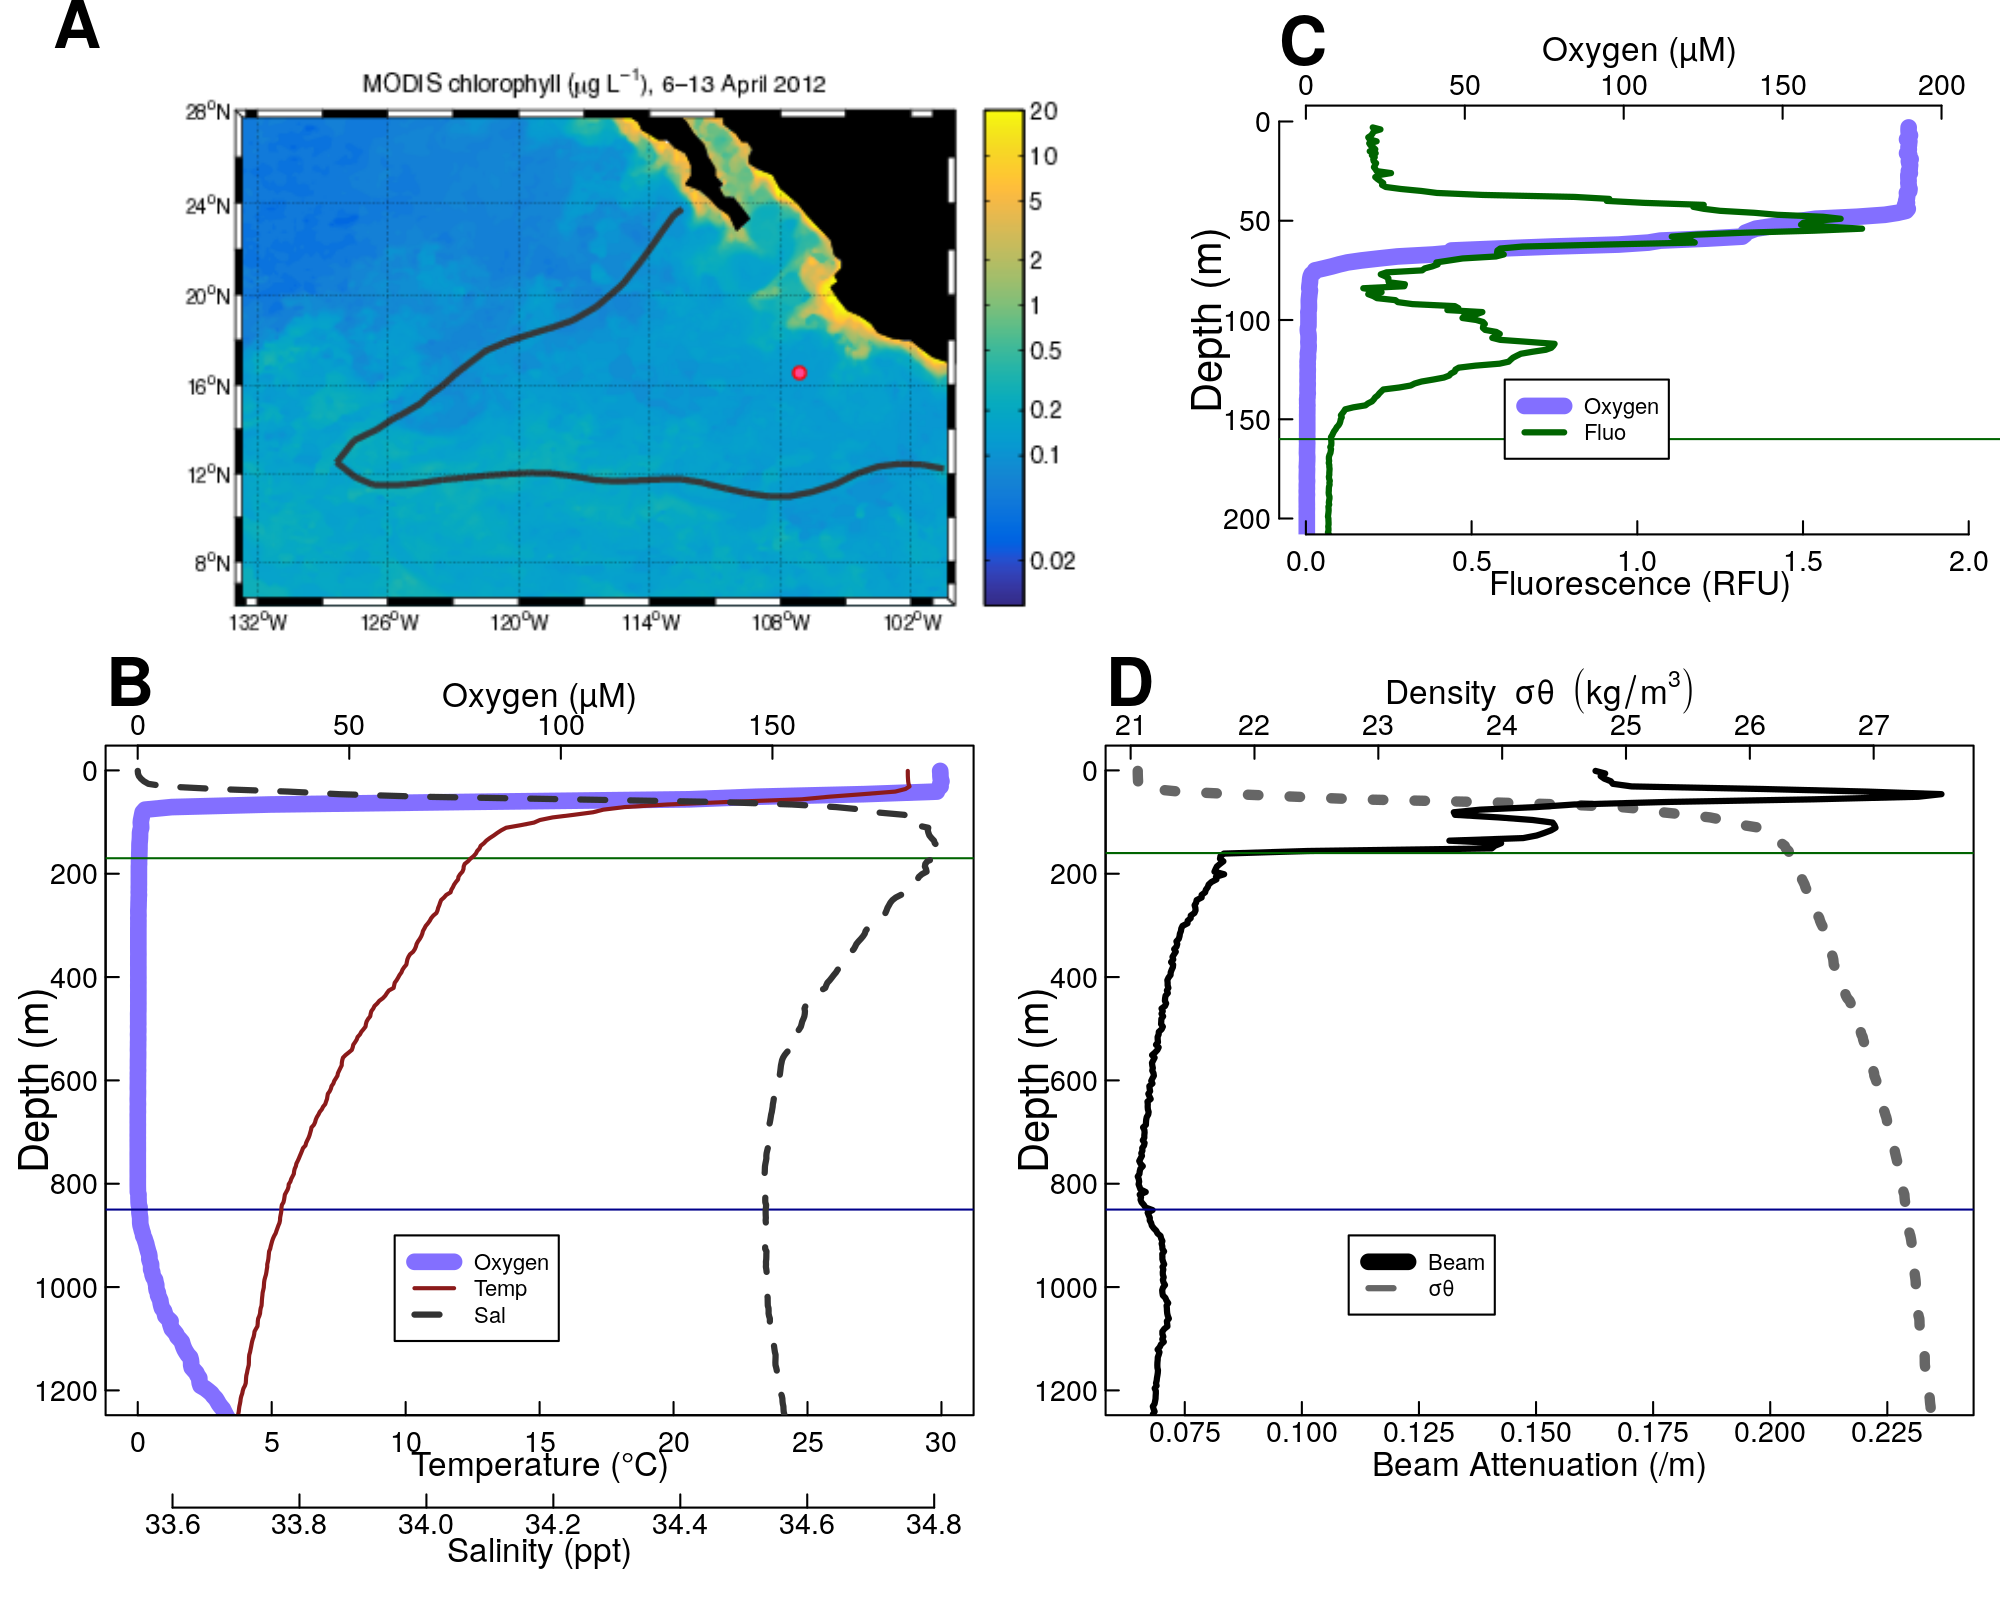
\includegraphics{../figures/CombinedP2Info.png}

Figure 1. Overview of the geography, physics and chemistry of ETNP
station P2 \textbf{(A)} Map of the ETNP Oxygen Minimum Zone and the
location of station P2. Colors indicate chlorophyll concentrations at
the surface, while the red outline signifies the region containing low
oxygen. The red circle indicates the location of Station P2. (B-D)
Oceanographic parameters collected from a cast at 2017-01-13 12:15 CST
(local time). All profiles contain a plot of oxygen concentrations. When
available, the thin horizontal green line shows the location of the base
of the photic zone (160m), while the horizontal blue line shows the base
of the oxycline. Figures B and D also show density (Dashed Gray Line).
(B) highlights temperature and salinity. (C) fluorescence, focusing on
the top 300m of the water column, and (D) beam attenuation.

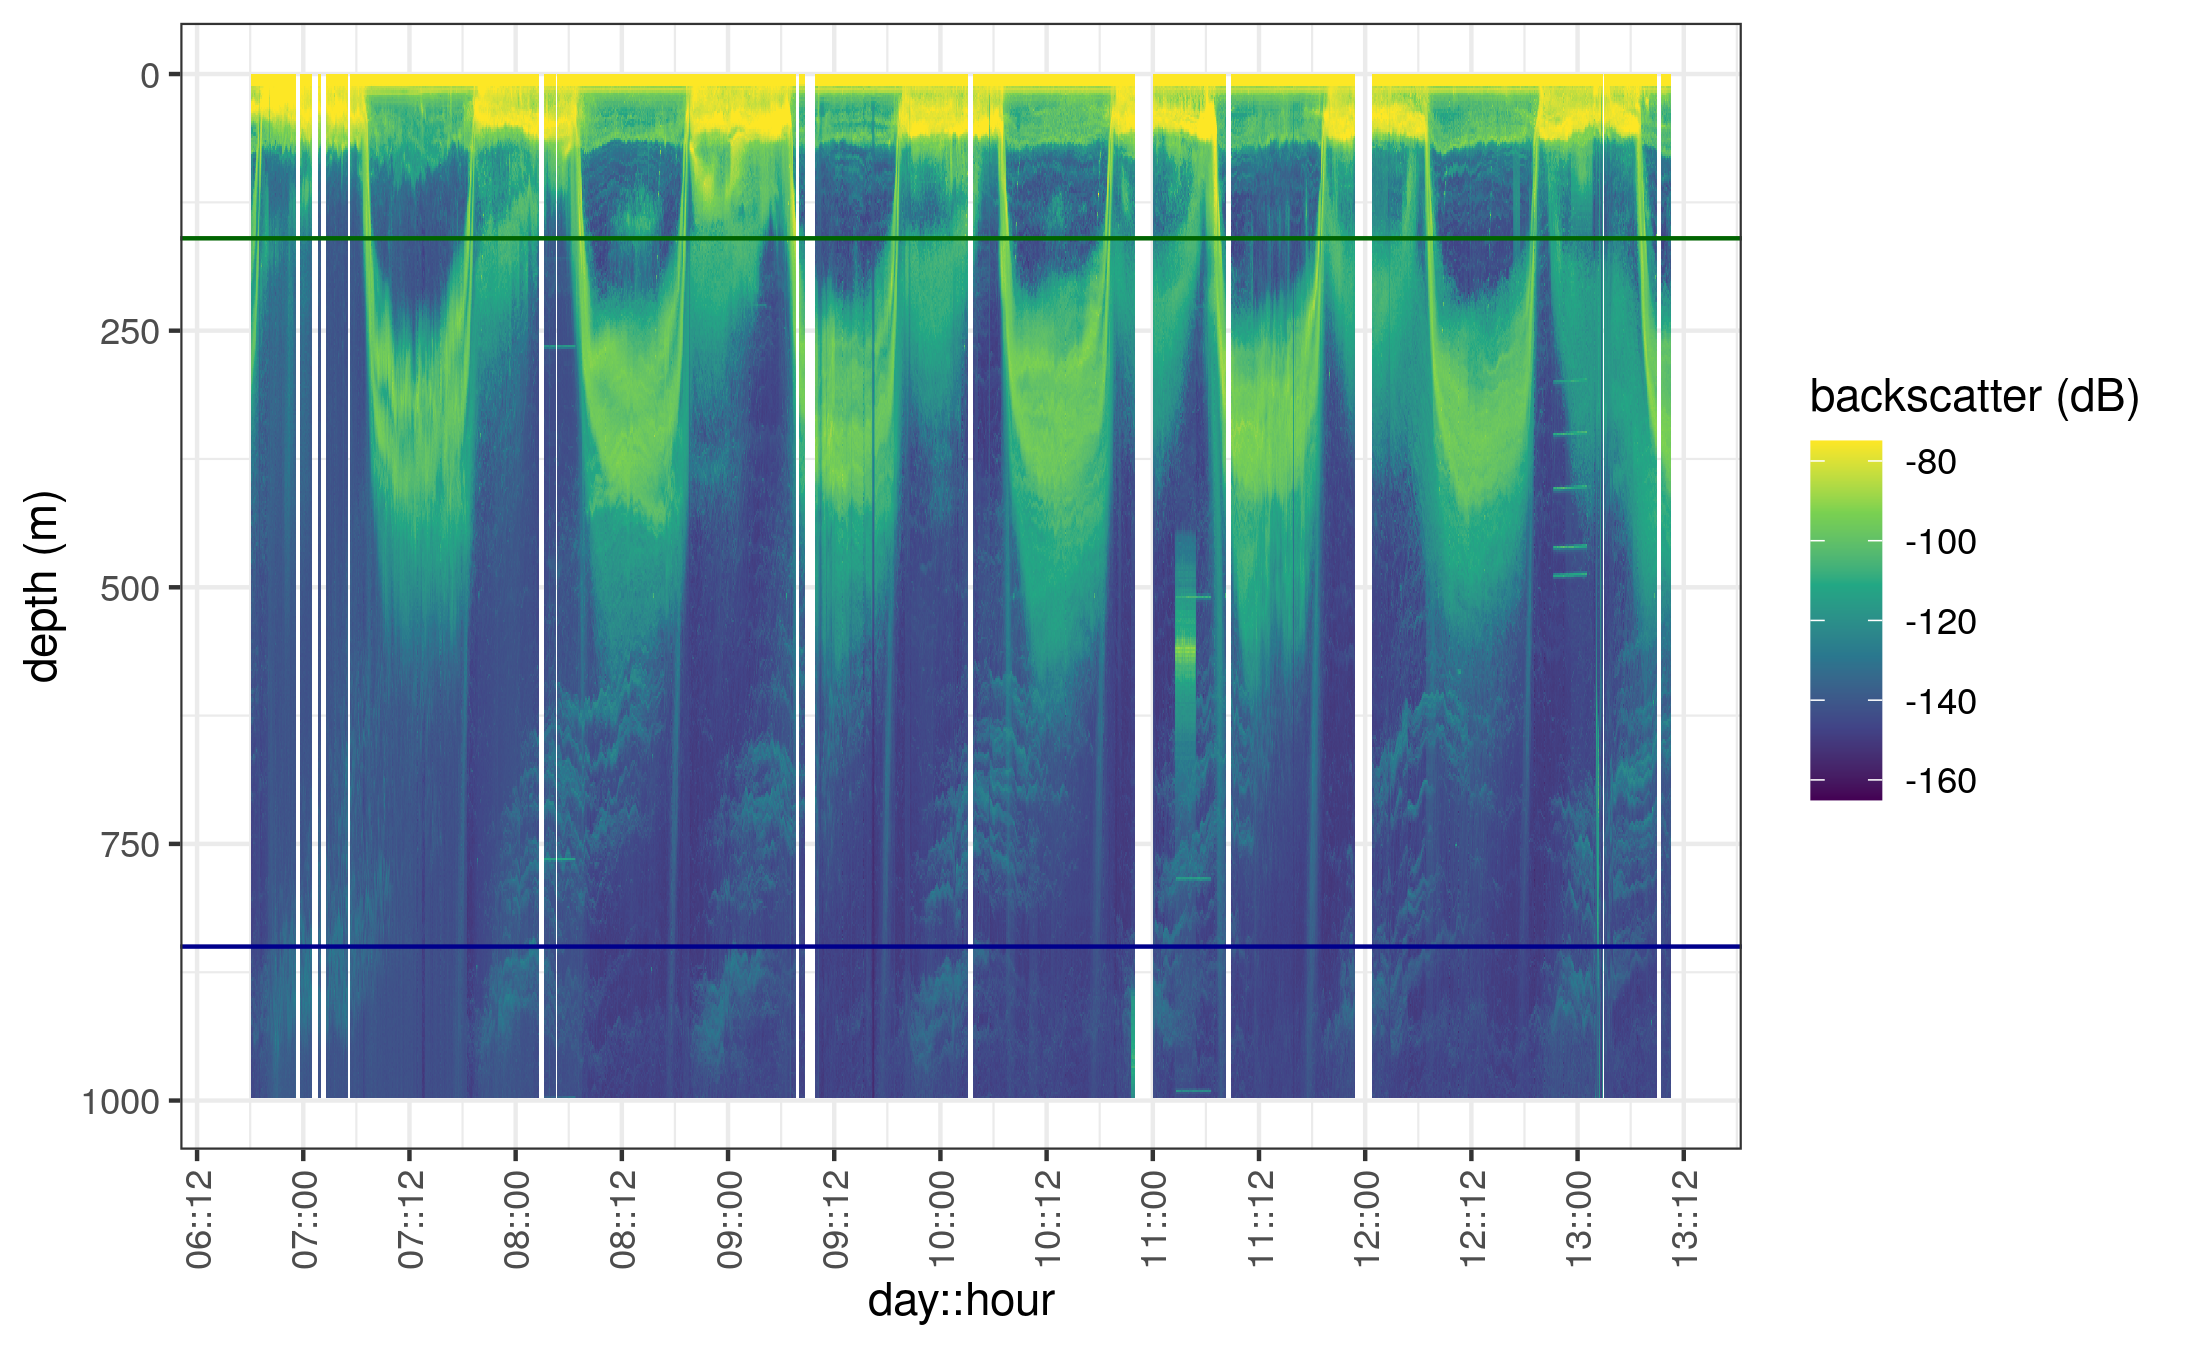
\includegraphics{../figures/stationP2_EK60_18kOnly.png}

Figure 2. Acoustic data, measured by EK60, measured over the course of
the experiment. Shown are data from the 18000 Hz frequency band, which
have highest depth penetration, but which appear to co-occur with data
from other frequency bands (see Figure S3). Values are in return signal
intensity and have not been normalized to observed biomass. Several
interesting patterns can be seen. \textbf{A.} Two bands of organisms can
be seen leaving the surface at dawn, spending the day between 250 and
500m and returning to the surface at dusk. \textbf{B.} Another group of
nocturnally migrating organisms can be seen leaving the surface at dusk,
spending the night near 250m and returning at dawn. \textbf{C.} Some
organisms appear at the base of the photic zone, during some, but not
all mid days, and then disappear in the evening. \textbf{D.} A group of
very deep migrating organisms appears to leave the surface with the diel
migrators and pass all the way through the ODZ and out of the EK60's
field of view. It returns at dusk. \textbf{E.} Swarms of organisms
appear between 500 and 1000m disappearing later in the day. Swarms
appear in the deepest layers at night and appear progressively shallower
as the day progresses.

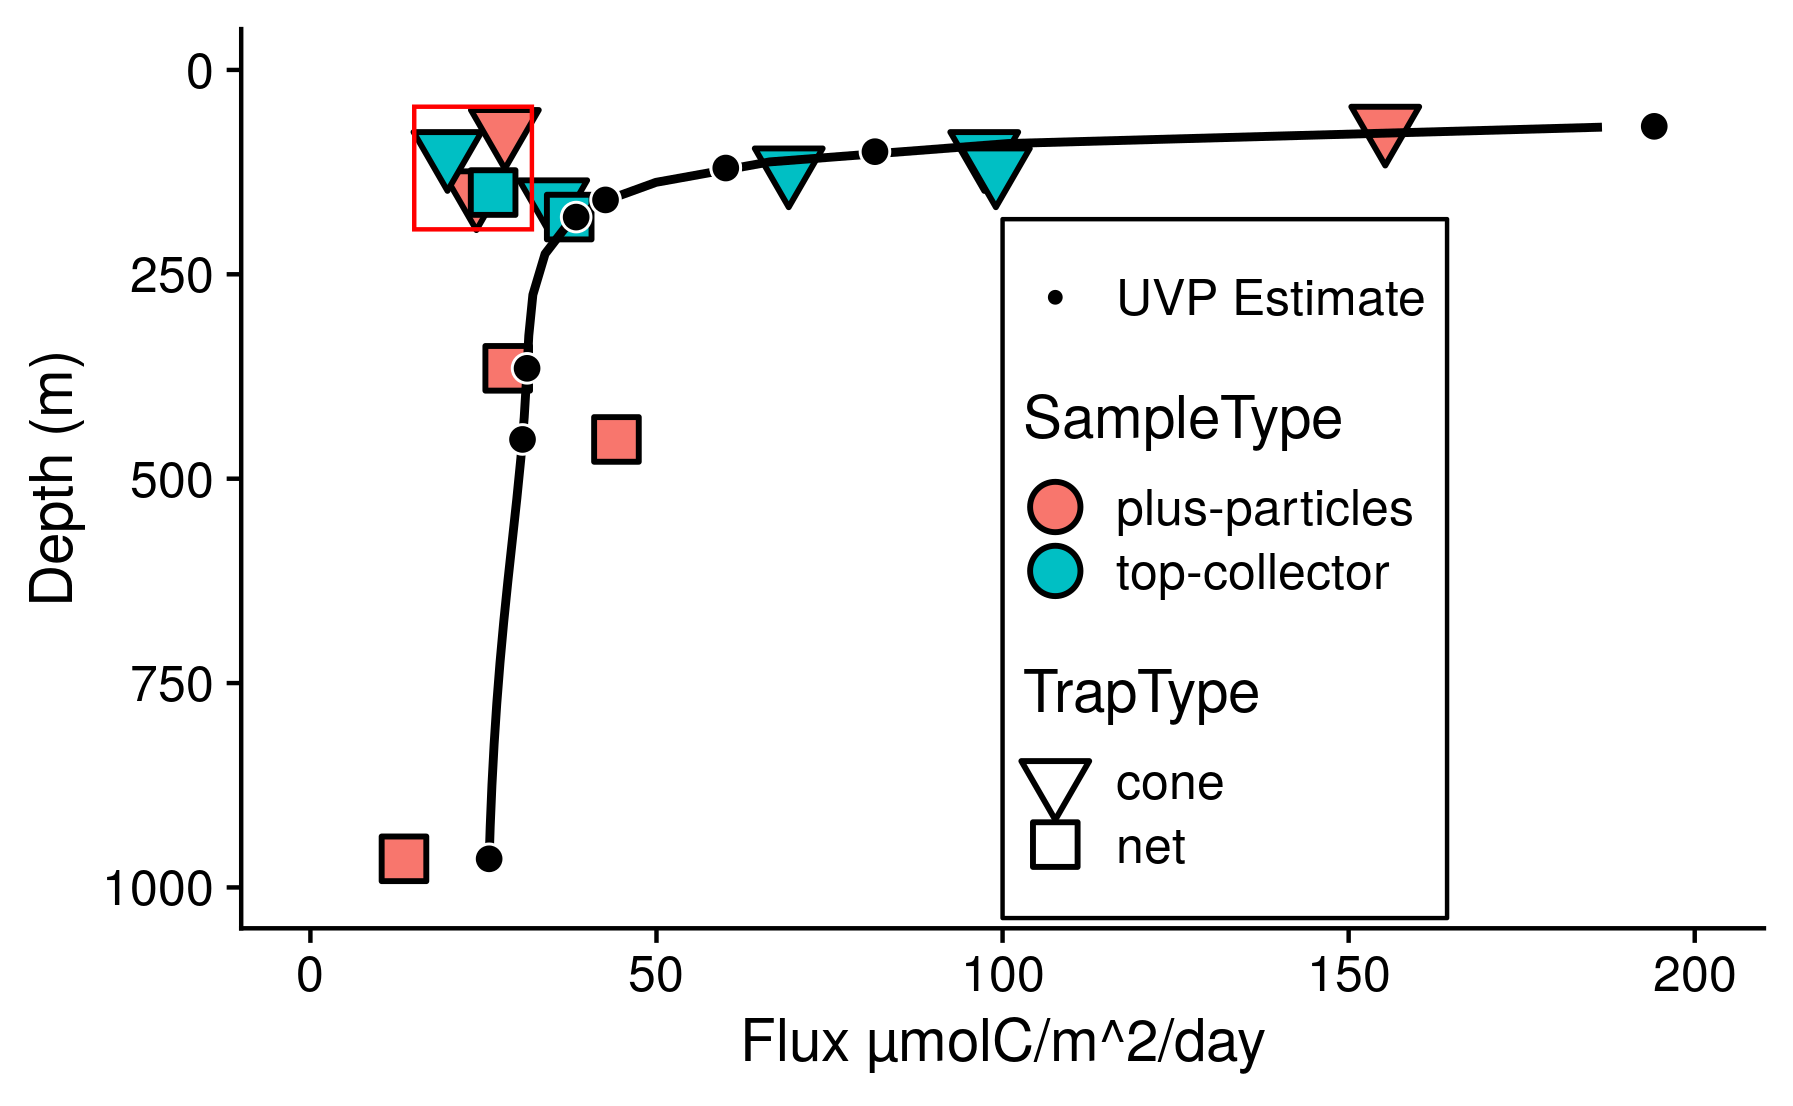
\includegraphics{../figures/FittedFlux.png}

Figure 3. Particle flux, measured from sinking traps large symbols. Data
from the ``plus particles'' and ``top collector'' samples from both cone
and net traps were collated to generate these data. Trap types are shown
by the shape and color of the large points. Superimposed are binned
estimates of particle flux generated by fitting the sum of particle
numbers all four profiles, binned as in Figure X, to the trap observed
flux. The four points enclosed by the rectangle are unusually low
compared to other traps collected at the same depth, and were therefore
excluded from the fit. \{Convert UVP points to a line, maybe leave
points where the traps ares\}

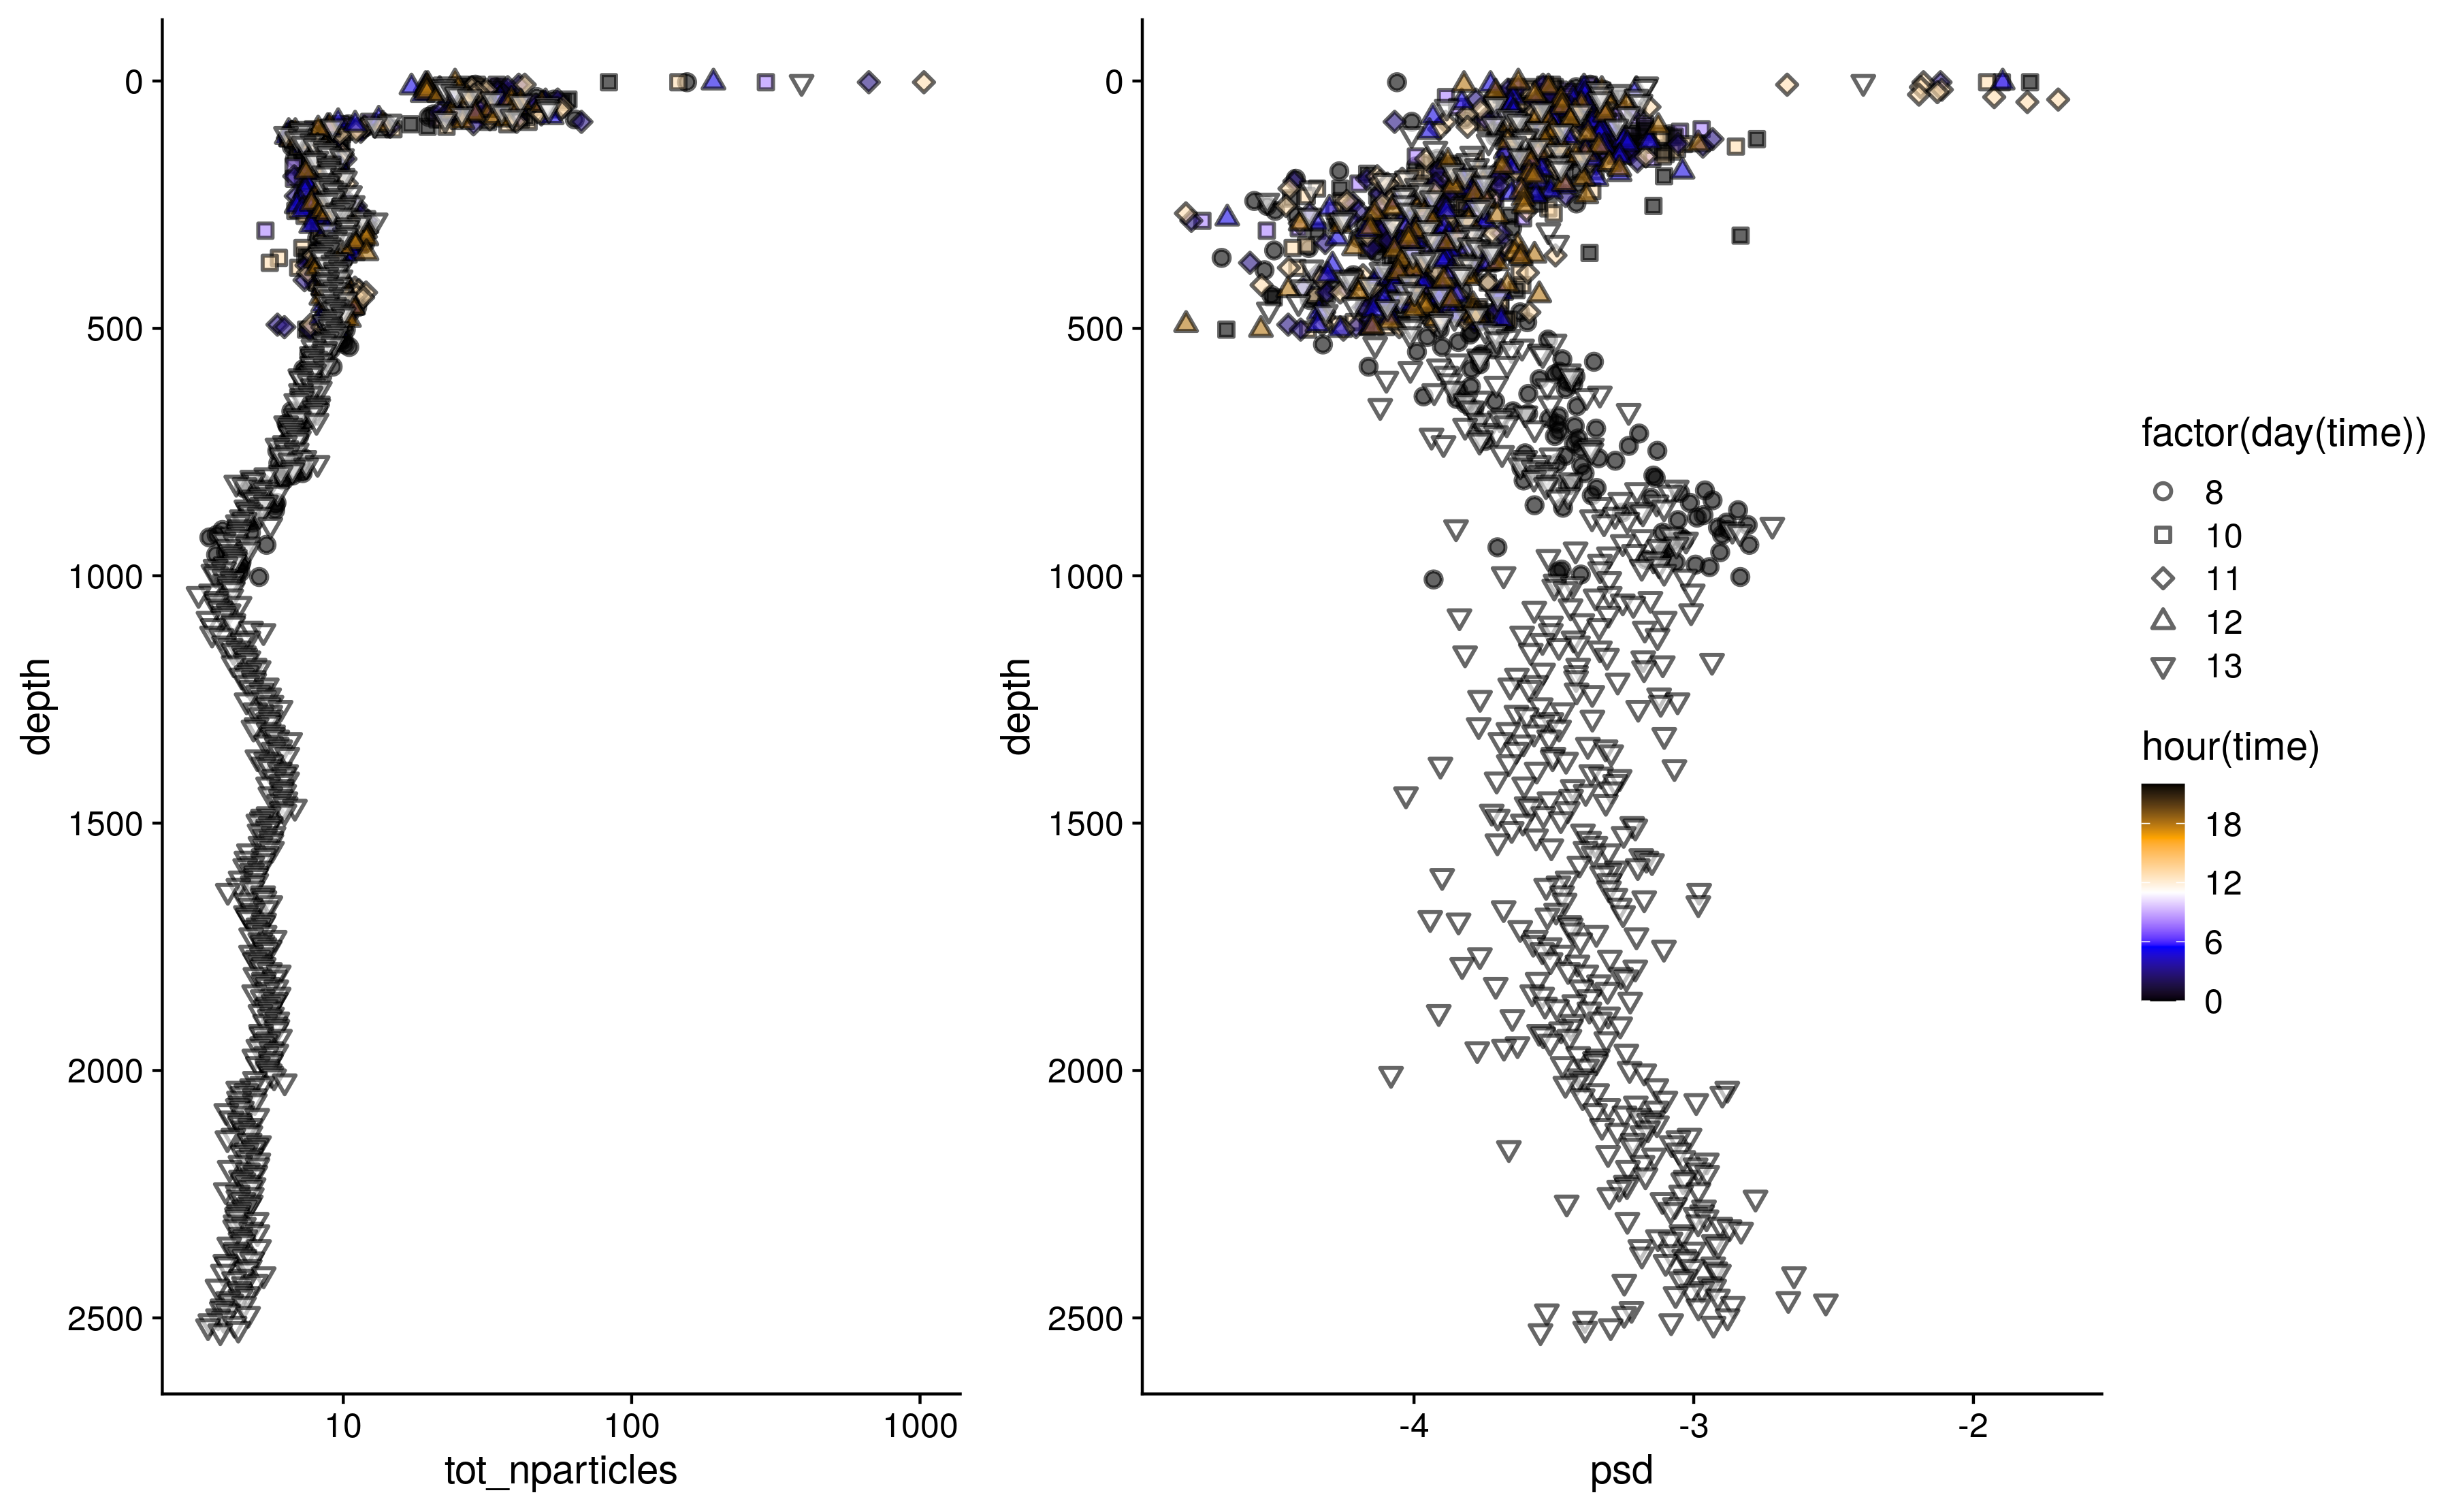
\includegraphics{../figures/ParticlesPSDMany.png}

Figure 4. (A) Observed, volume normalized total particle numbers from 9
casts taken at different times of the day at ETNP station P2. (B)
Calculated particle size distribution slopes of those particles. These
data have not been binned by depth.

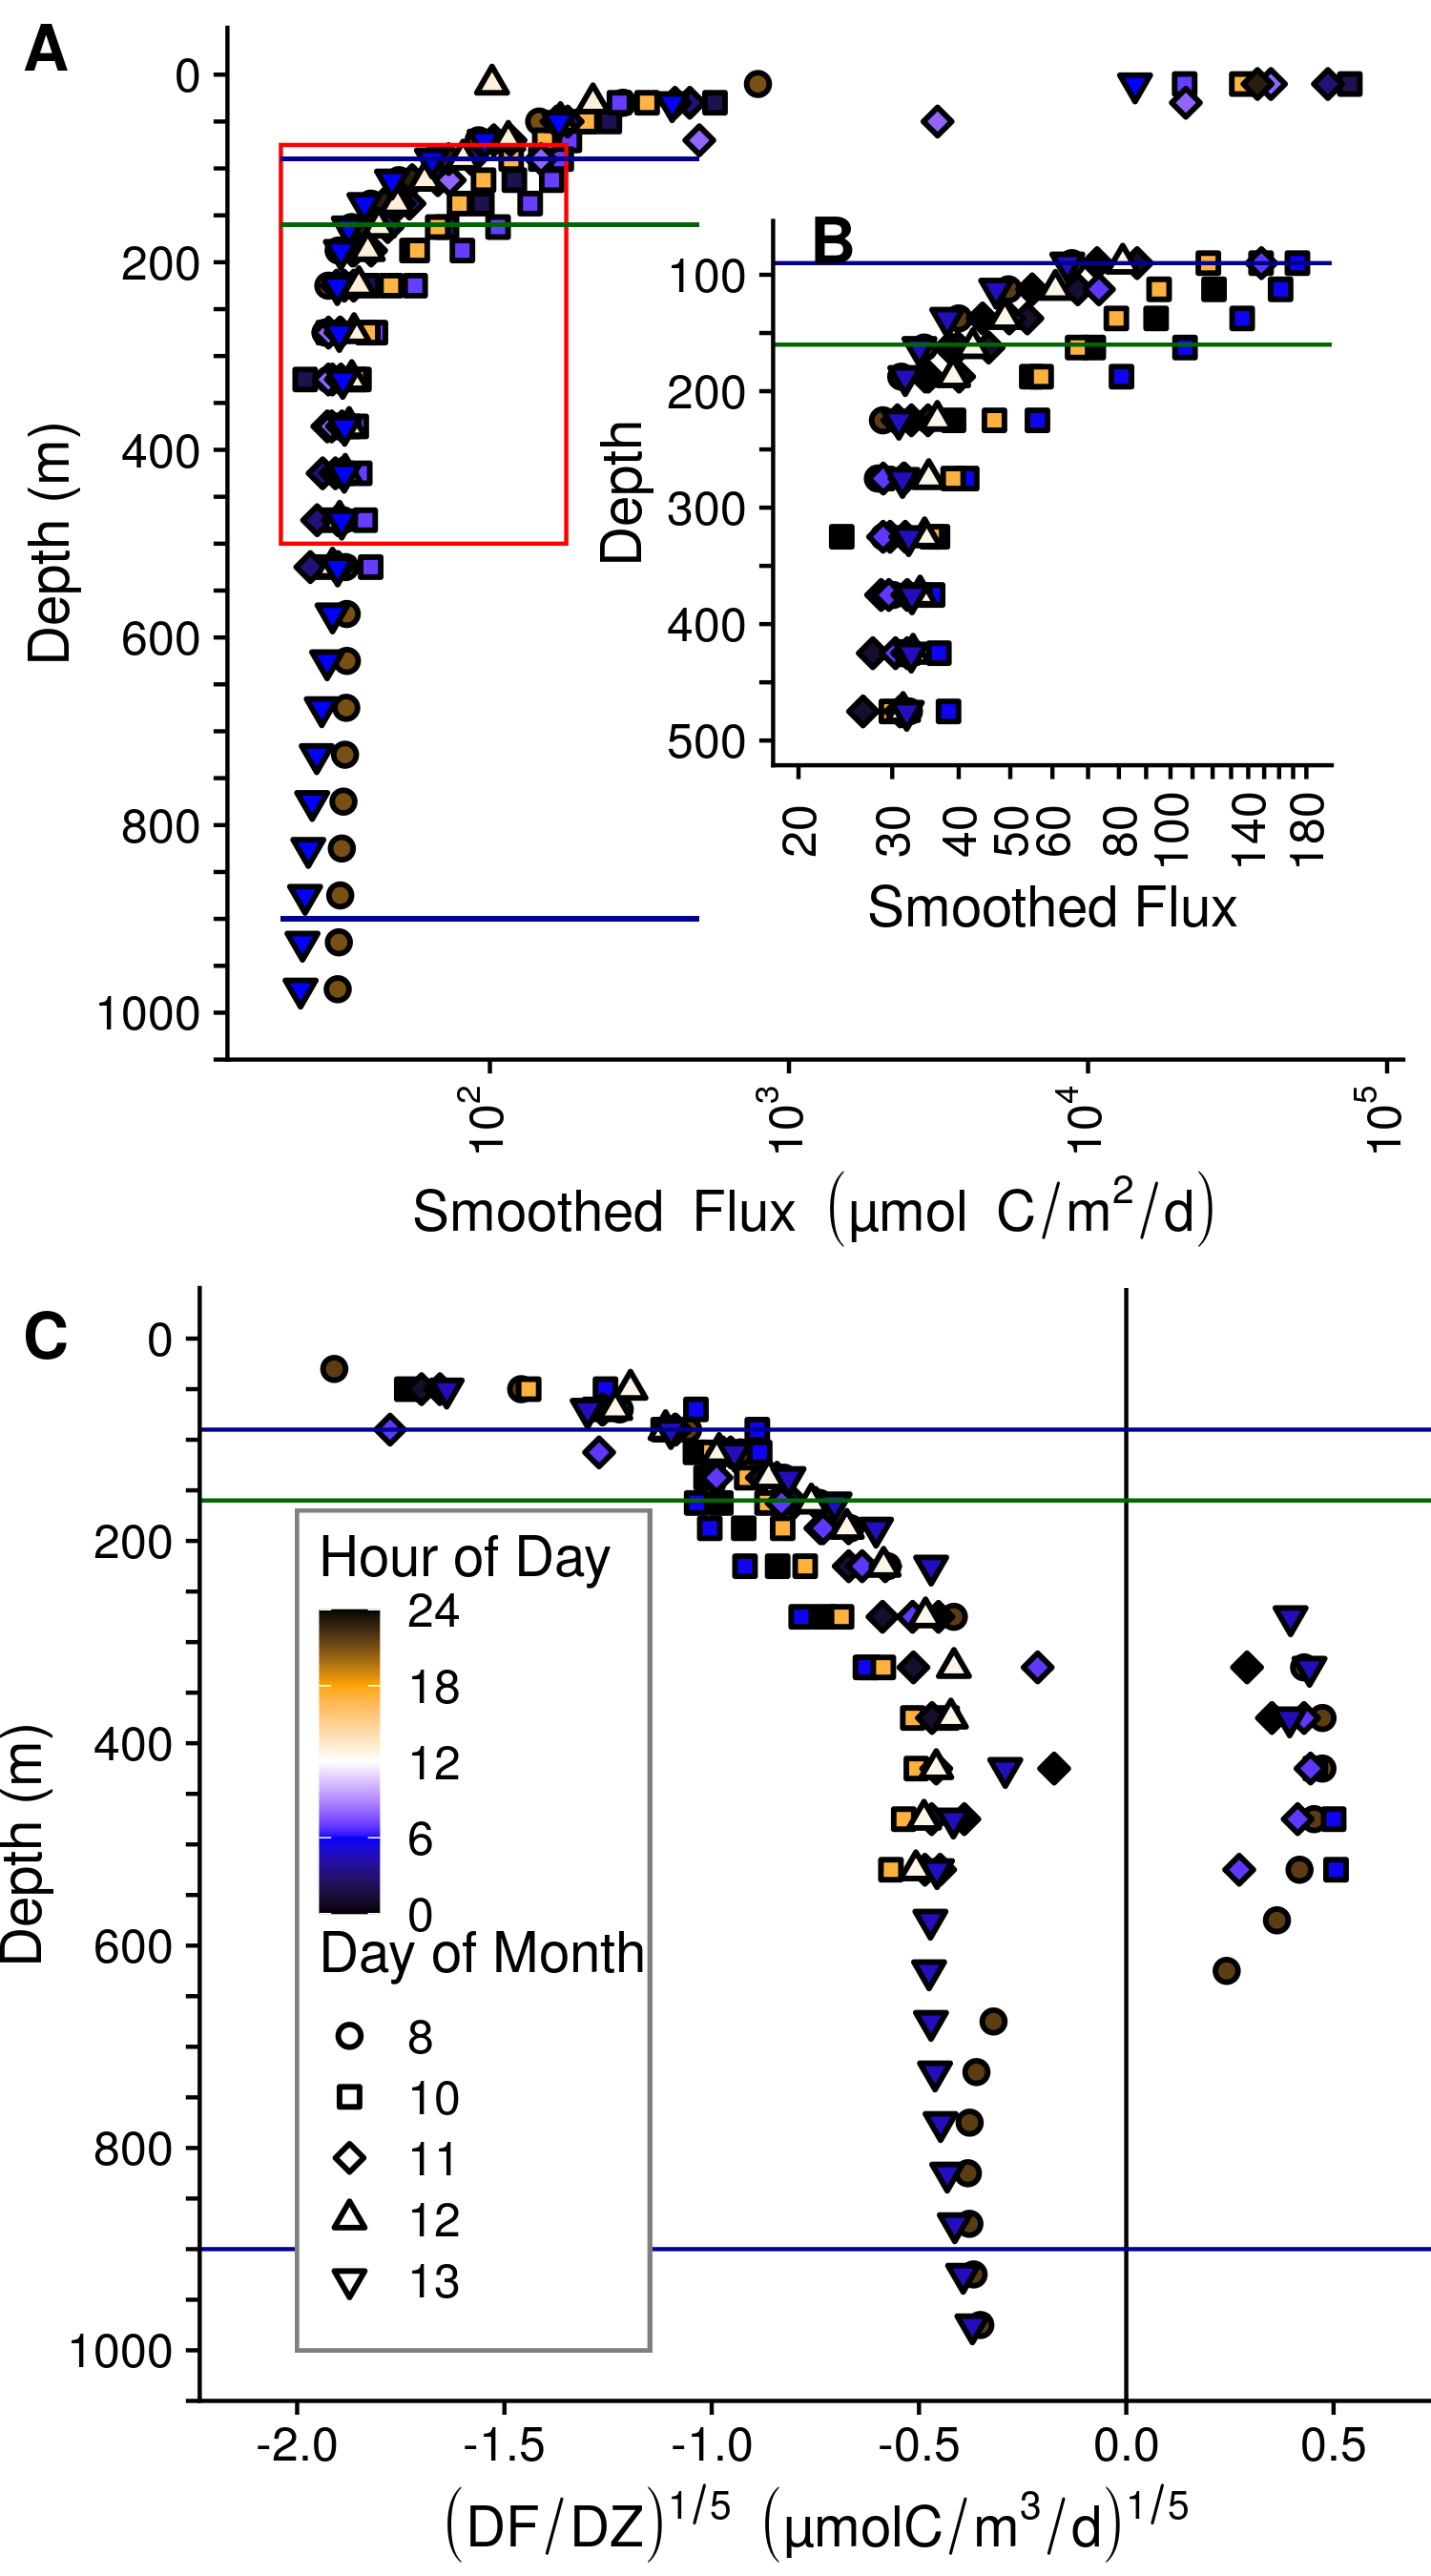
\includegraphics{../figures/FluxDeepDive.png}

Figure 5. Within and between day variability in UVP predicted particle
flux at ETNP station P2. Profiles are compared against P16 station 100,
a non ODZ station at similar latitude in the tropical pacific. All
profiles are depth binned with higher resolution towards the surface
(methods). \textbf{(A)} Flux profiles in the top 1000m of the water
column. \textbf{(B)} A more detailed depiction of the area enclosed by
the rectangle in \textbf{A}. \textbf{(C)} The rate of change of flux,
divided by the rate in change in depth. We show the fifth root of these
values in order to highlight differences between values close to zero.

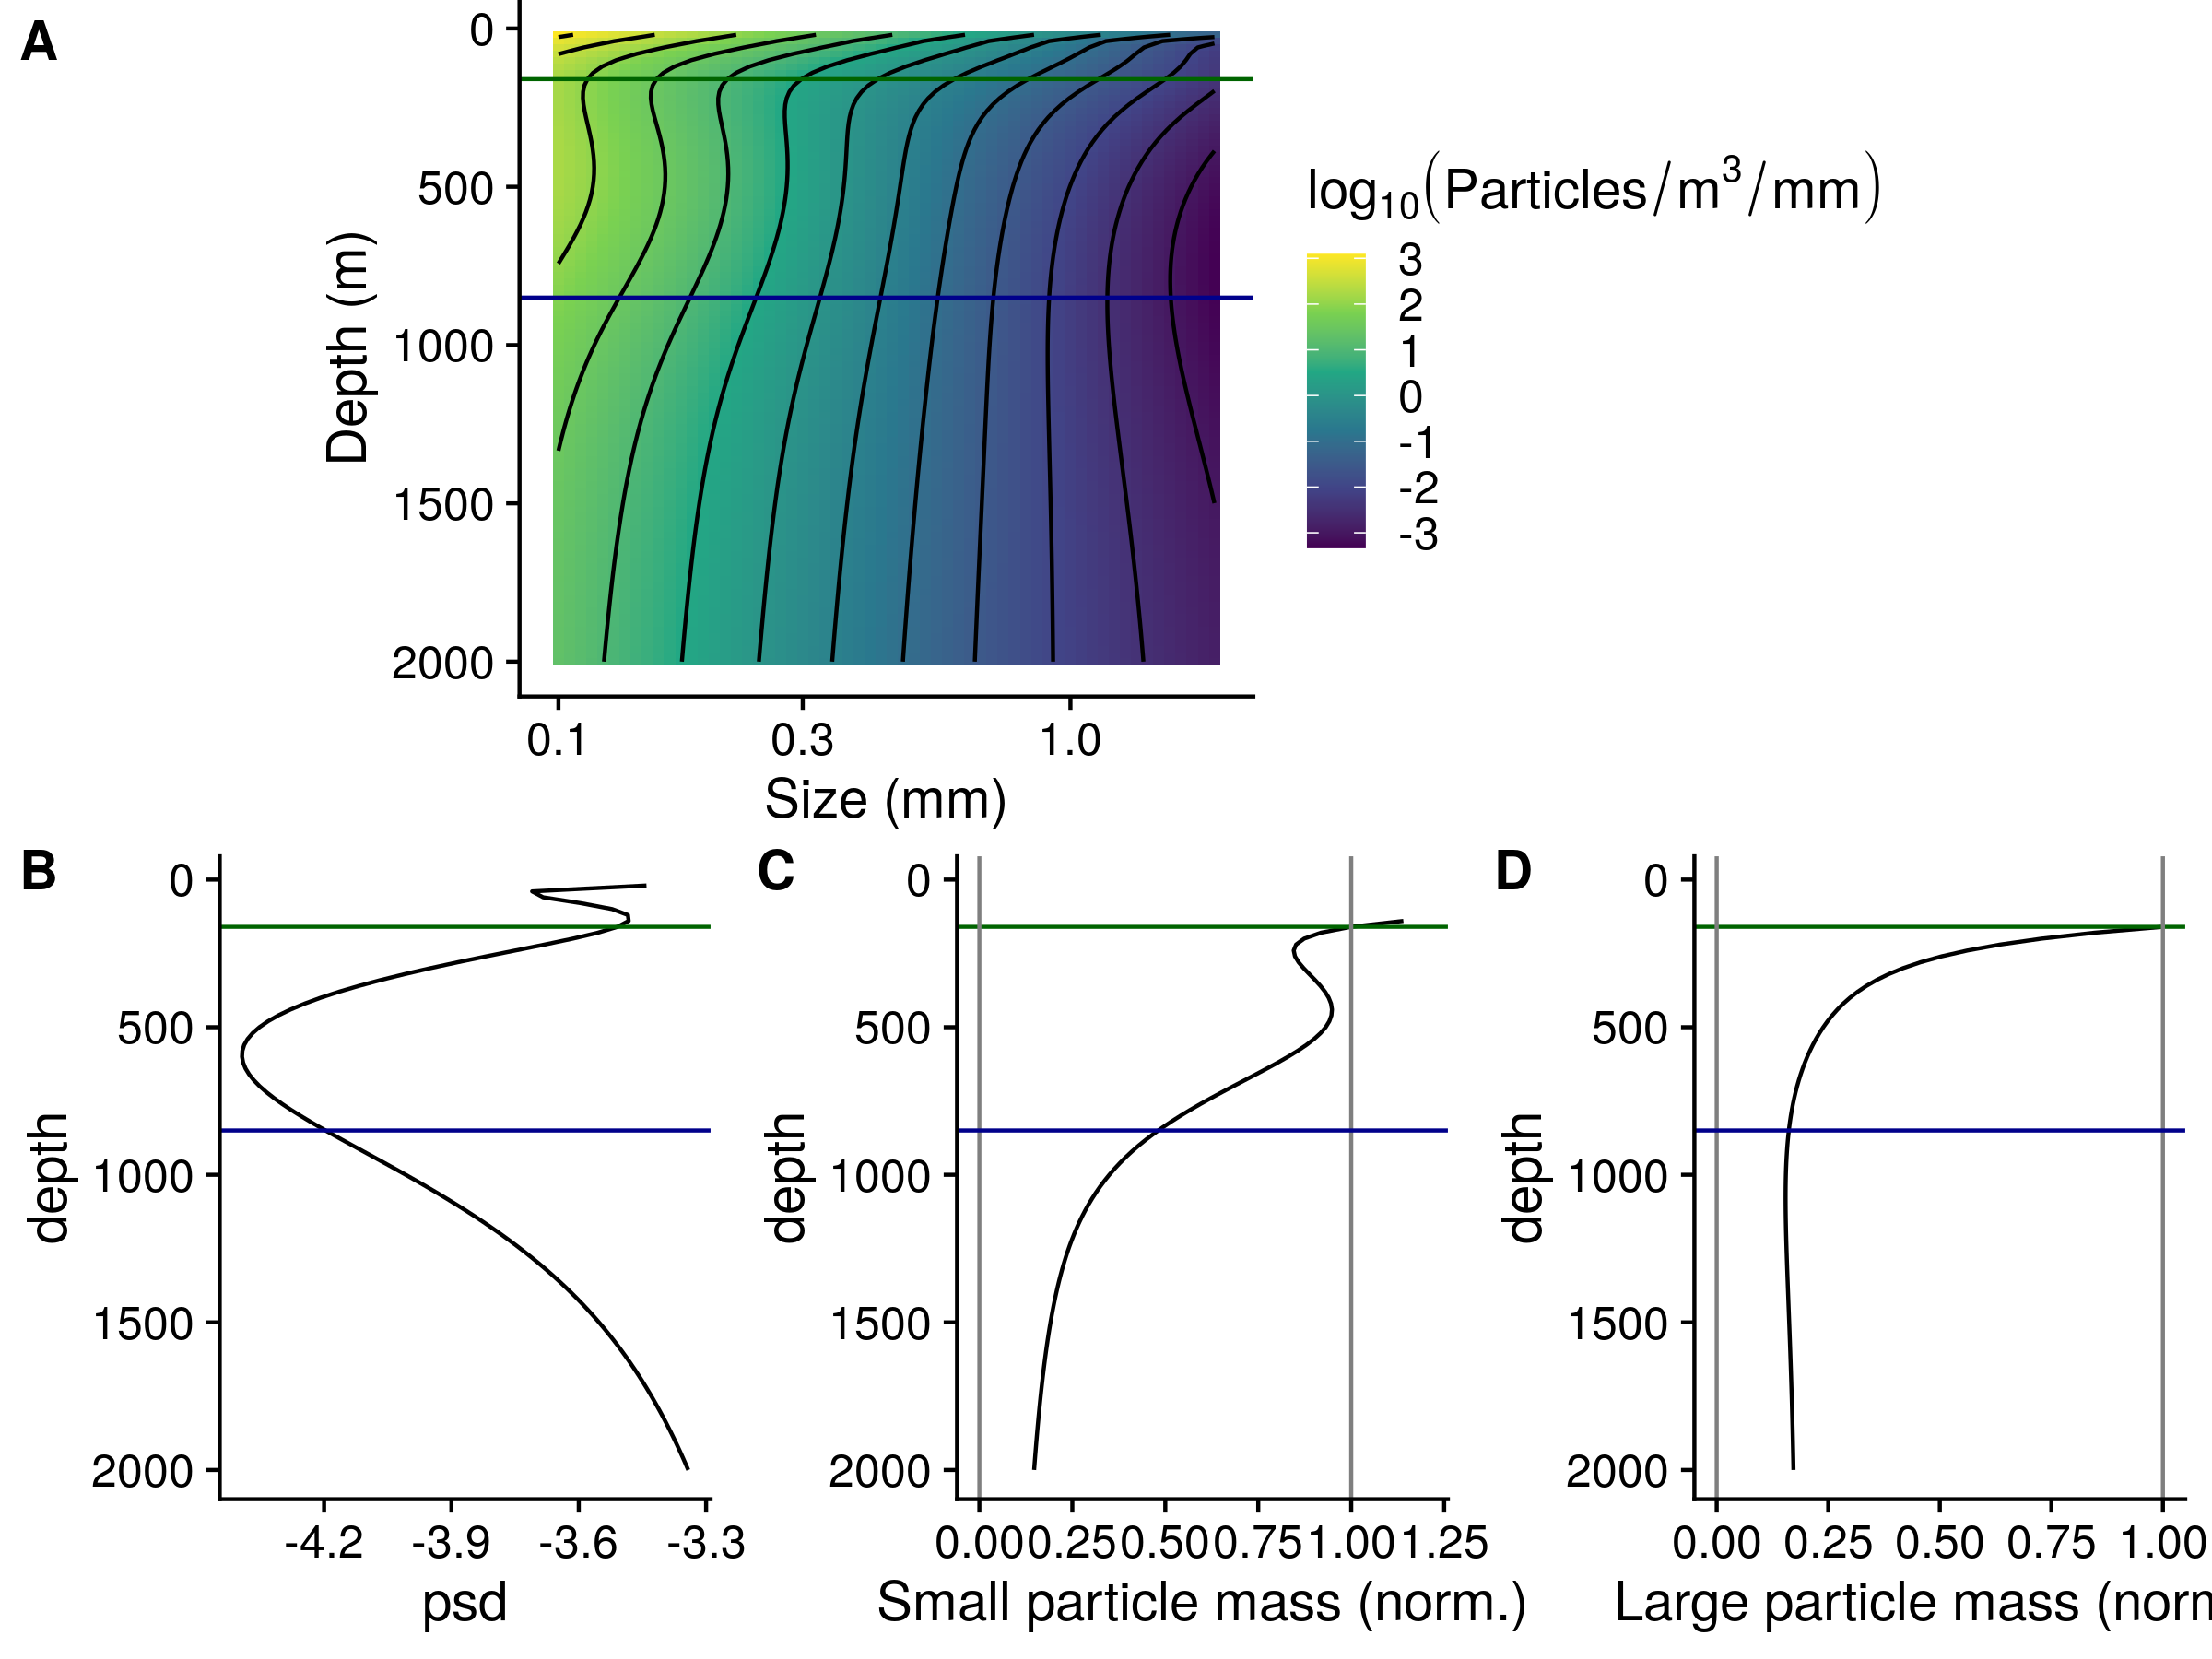
\includegraphics{../figures/WBModelValidation.png}

Figure 6. \textbf{(A)} GAM smoothed bin-size and volume particle numbers
at each particle size class. \textbf{(B)} Particle size distributions.
And estimated biomass of \textbf{(C)} Small and \textbf{(D)} Large
particles.

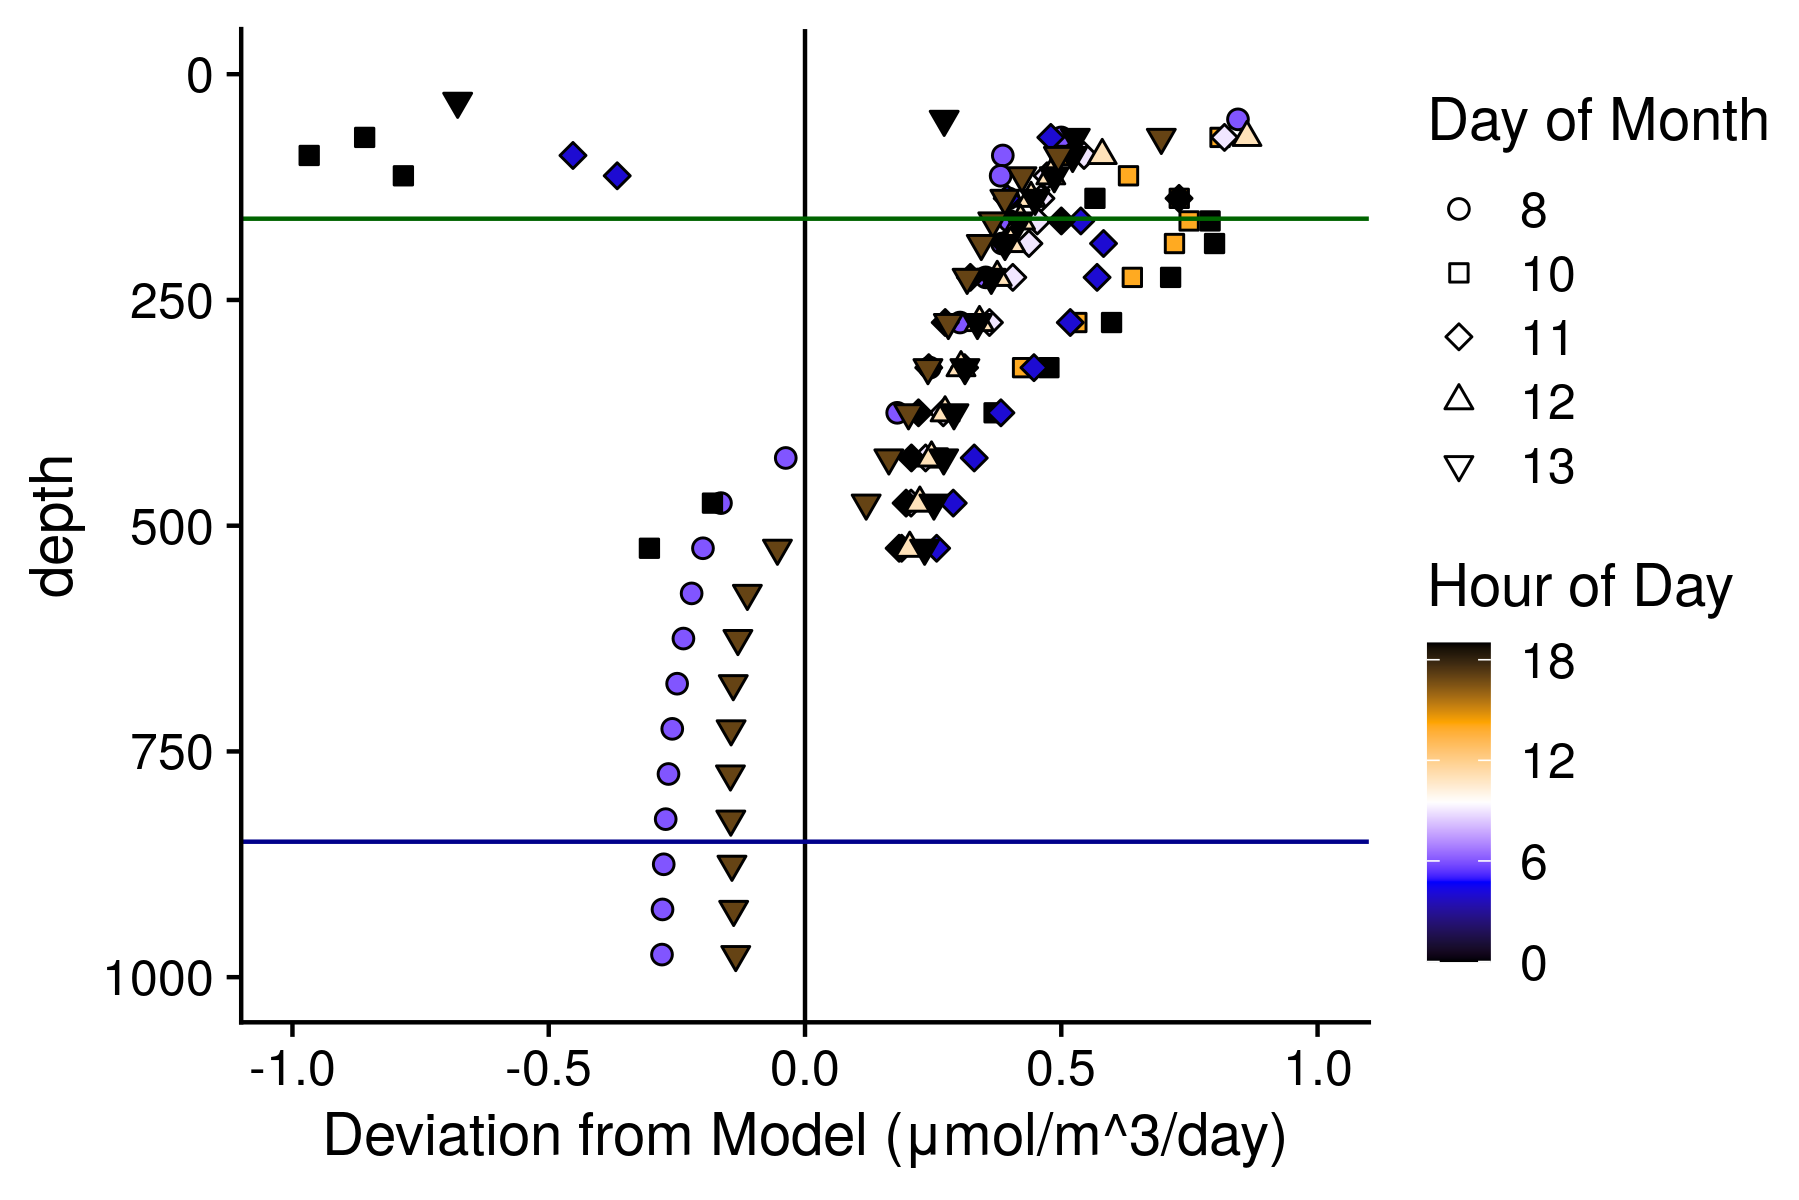
\includegraphics{../figures/FluxSizeShift.png} Figure 7. Quantification
of non remineralization and sinking like processes. \emph{Deviation from
Model} indicates the difference between the observed small particle
flux, and the flux that would be estimated if particles from the size
distribution in the depth bin above remineralized and sank only
following the PRiSM model. Values are normalized to the change in depth.
Thus values are \(\mu\)mol Carbon/m3/day.

\hypertarget{supplemental-figs}{%
\section{Supplemental Figs}\label{supplemental-figs}}

{[}move to supplement{]}

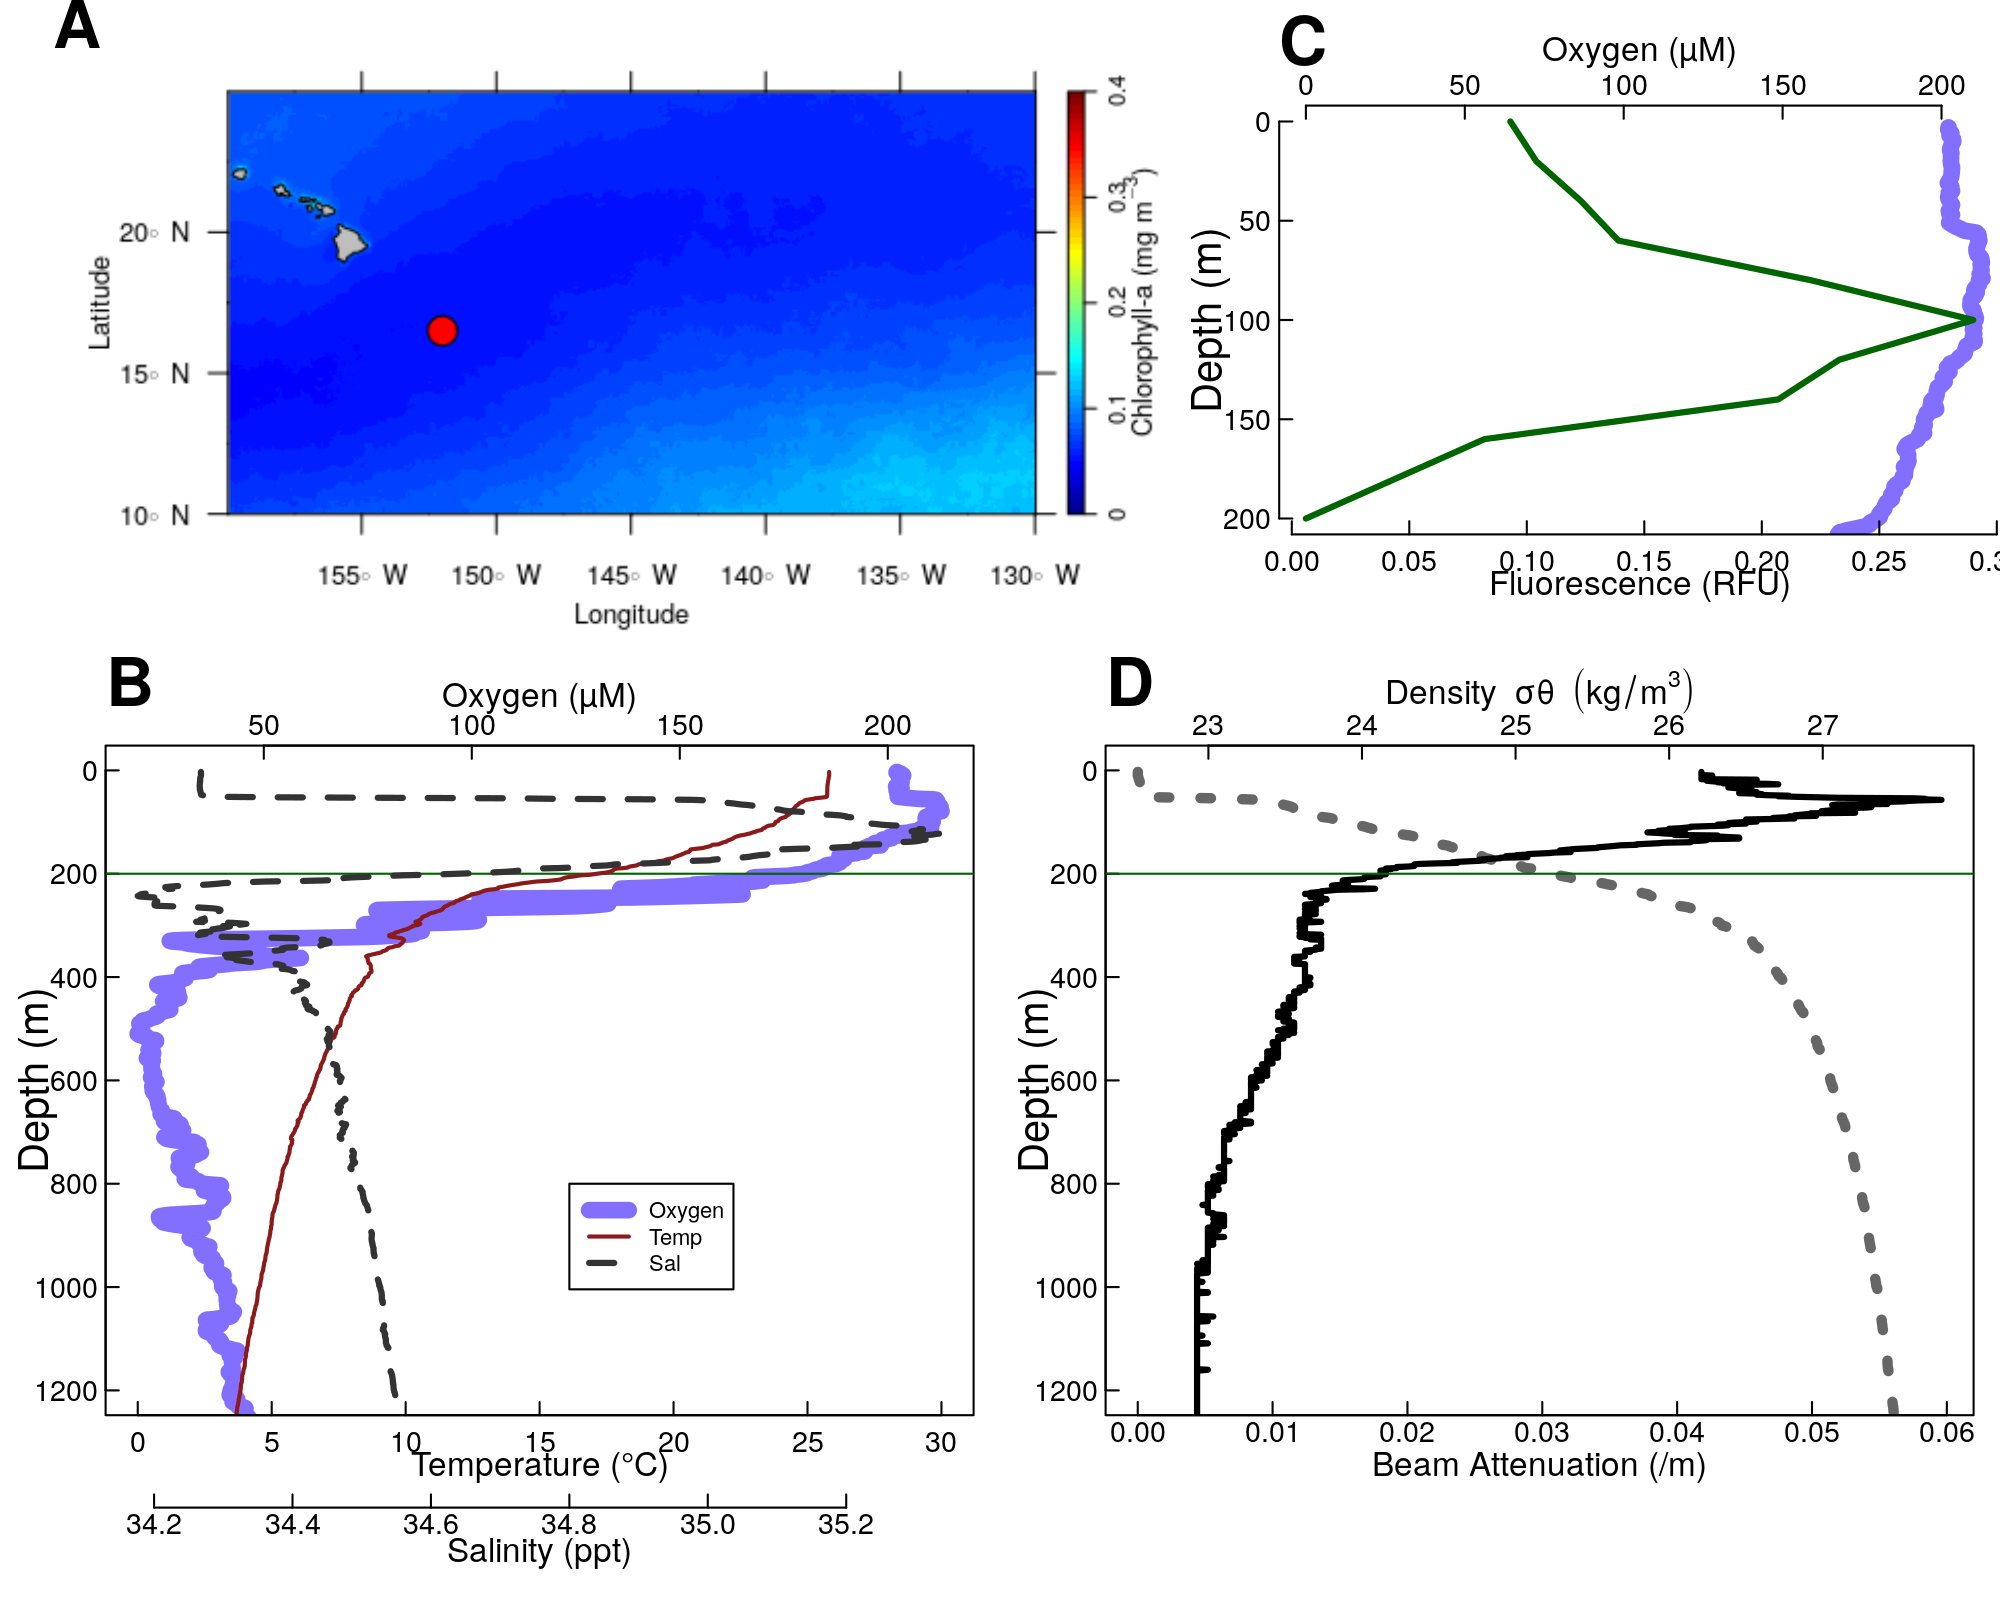
\includegraphics{../figures/CombinedP16S100Info.png}

Figure S1. Physical and chemical data from P16 Station 100. Located at
16.5°N 152.0°W. (A) Map of the nearby tropical pacific station P6
Station 100. Colors indicate chlorophyll concentrations at the surface,
averaged over all MODIS images. The red circle indicates the location of
Station P2. (B-D) Oceanographic parameters. The thin horizontal green
line shows the location of the base of the photic zone (200m m).
\textbf{A} Oxygen, and fluorescence. Because the fluorometer was broken
on this cruise, fluorescence data were pulled from world ocean atlas.
\textbf{B} Oxygen temperature and salinity. \textbf{(C)} Beam
attenuation and density, calculated from the salinity temperature and
pressure data.

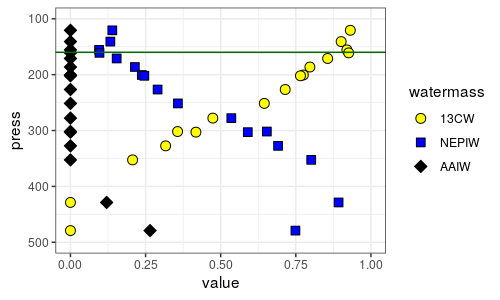
\includegraphics{../figures/evans16p5N107W.png} Figure S2. Water mass
analyis indicates the relative contributions proportions of the three
primary water masses at this site, \(13^\circ C\) water (13CW), North
Equitorial Pacific Intermediate Water (NEPIW) and Antarctic Intermediate
Water(AAIW). Values indicate relative contributions of each water mass
and are scaled so as to sum to one. Data are taken directly from Evans
et al. (2020).

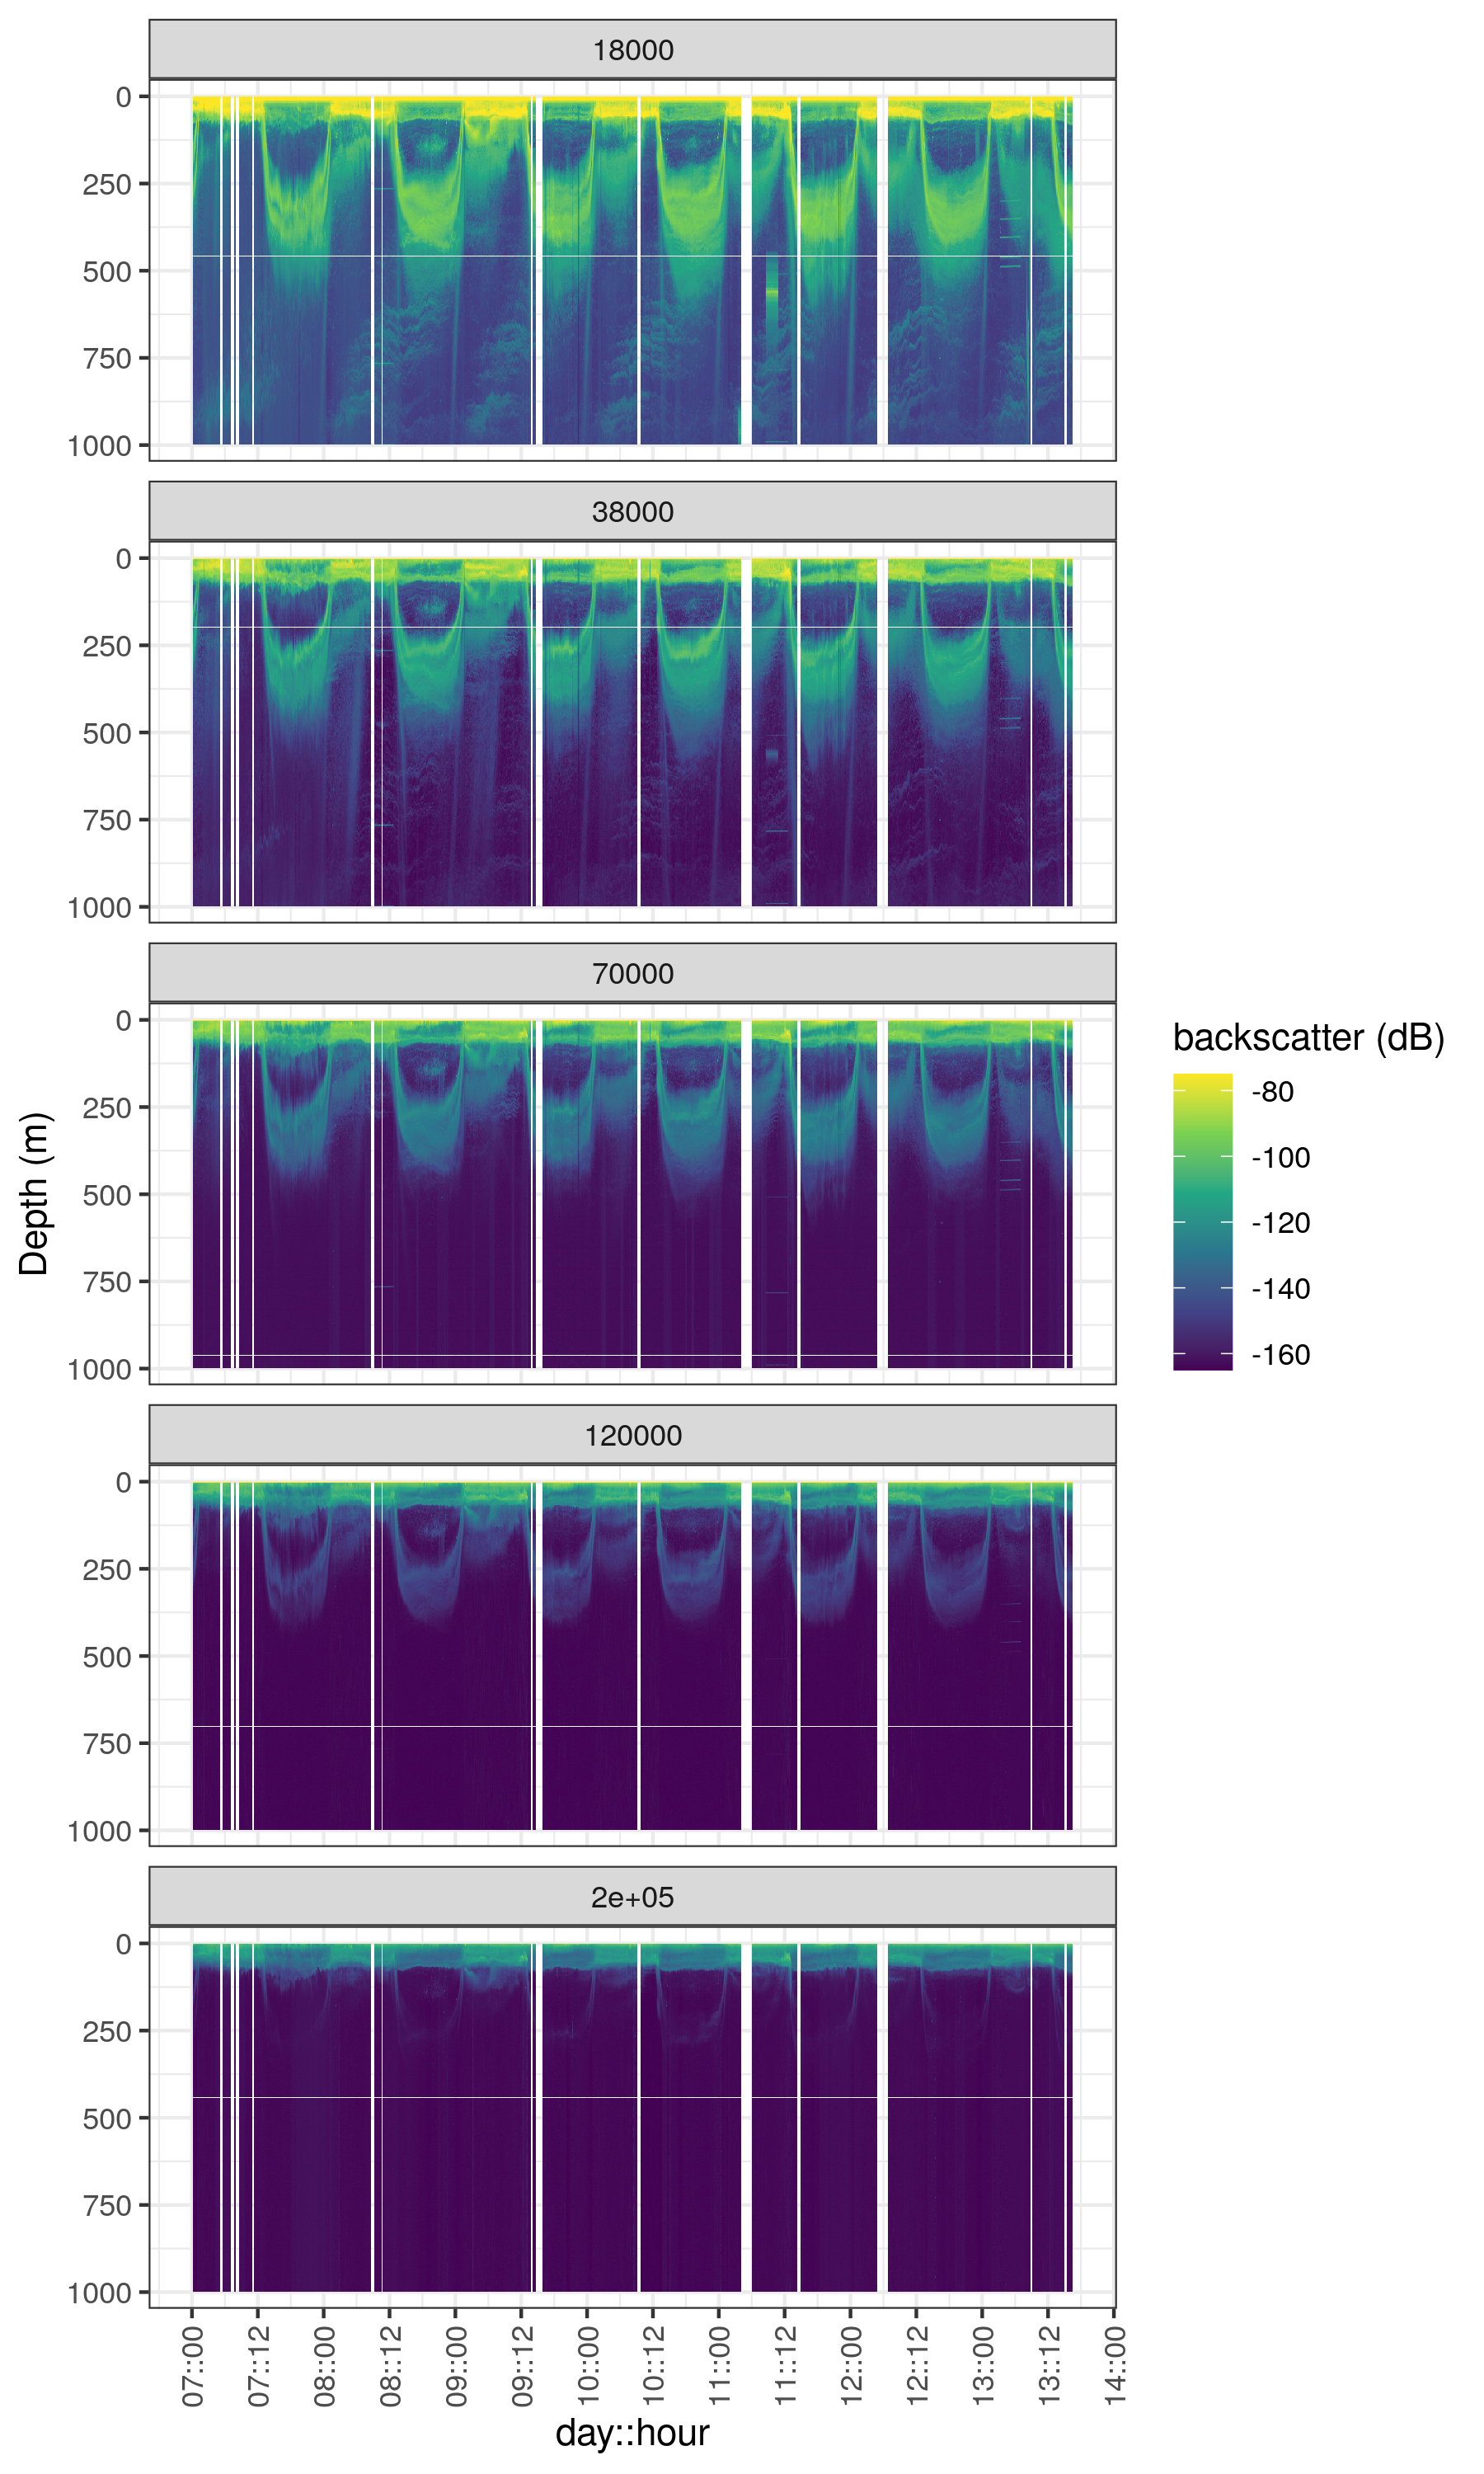
\includegraphics{../figures/stationP2_EK60_go7.png}

Figure S3. Acoustic data, measured by EK60, measured over the course of
the experiment. Shown are data from the all frequency bands. Values are
in return signal intensity and have not been normalized to observed
biomass.

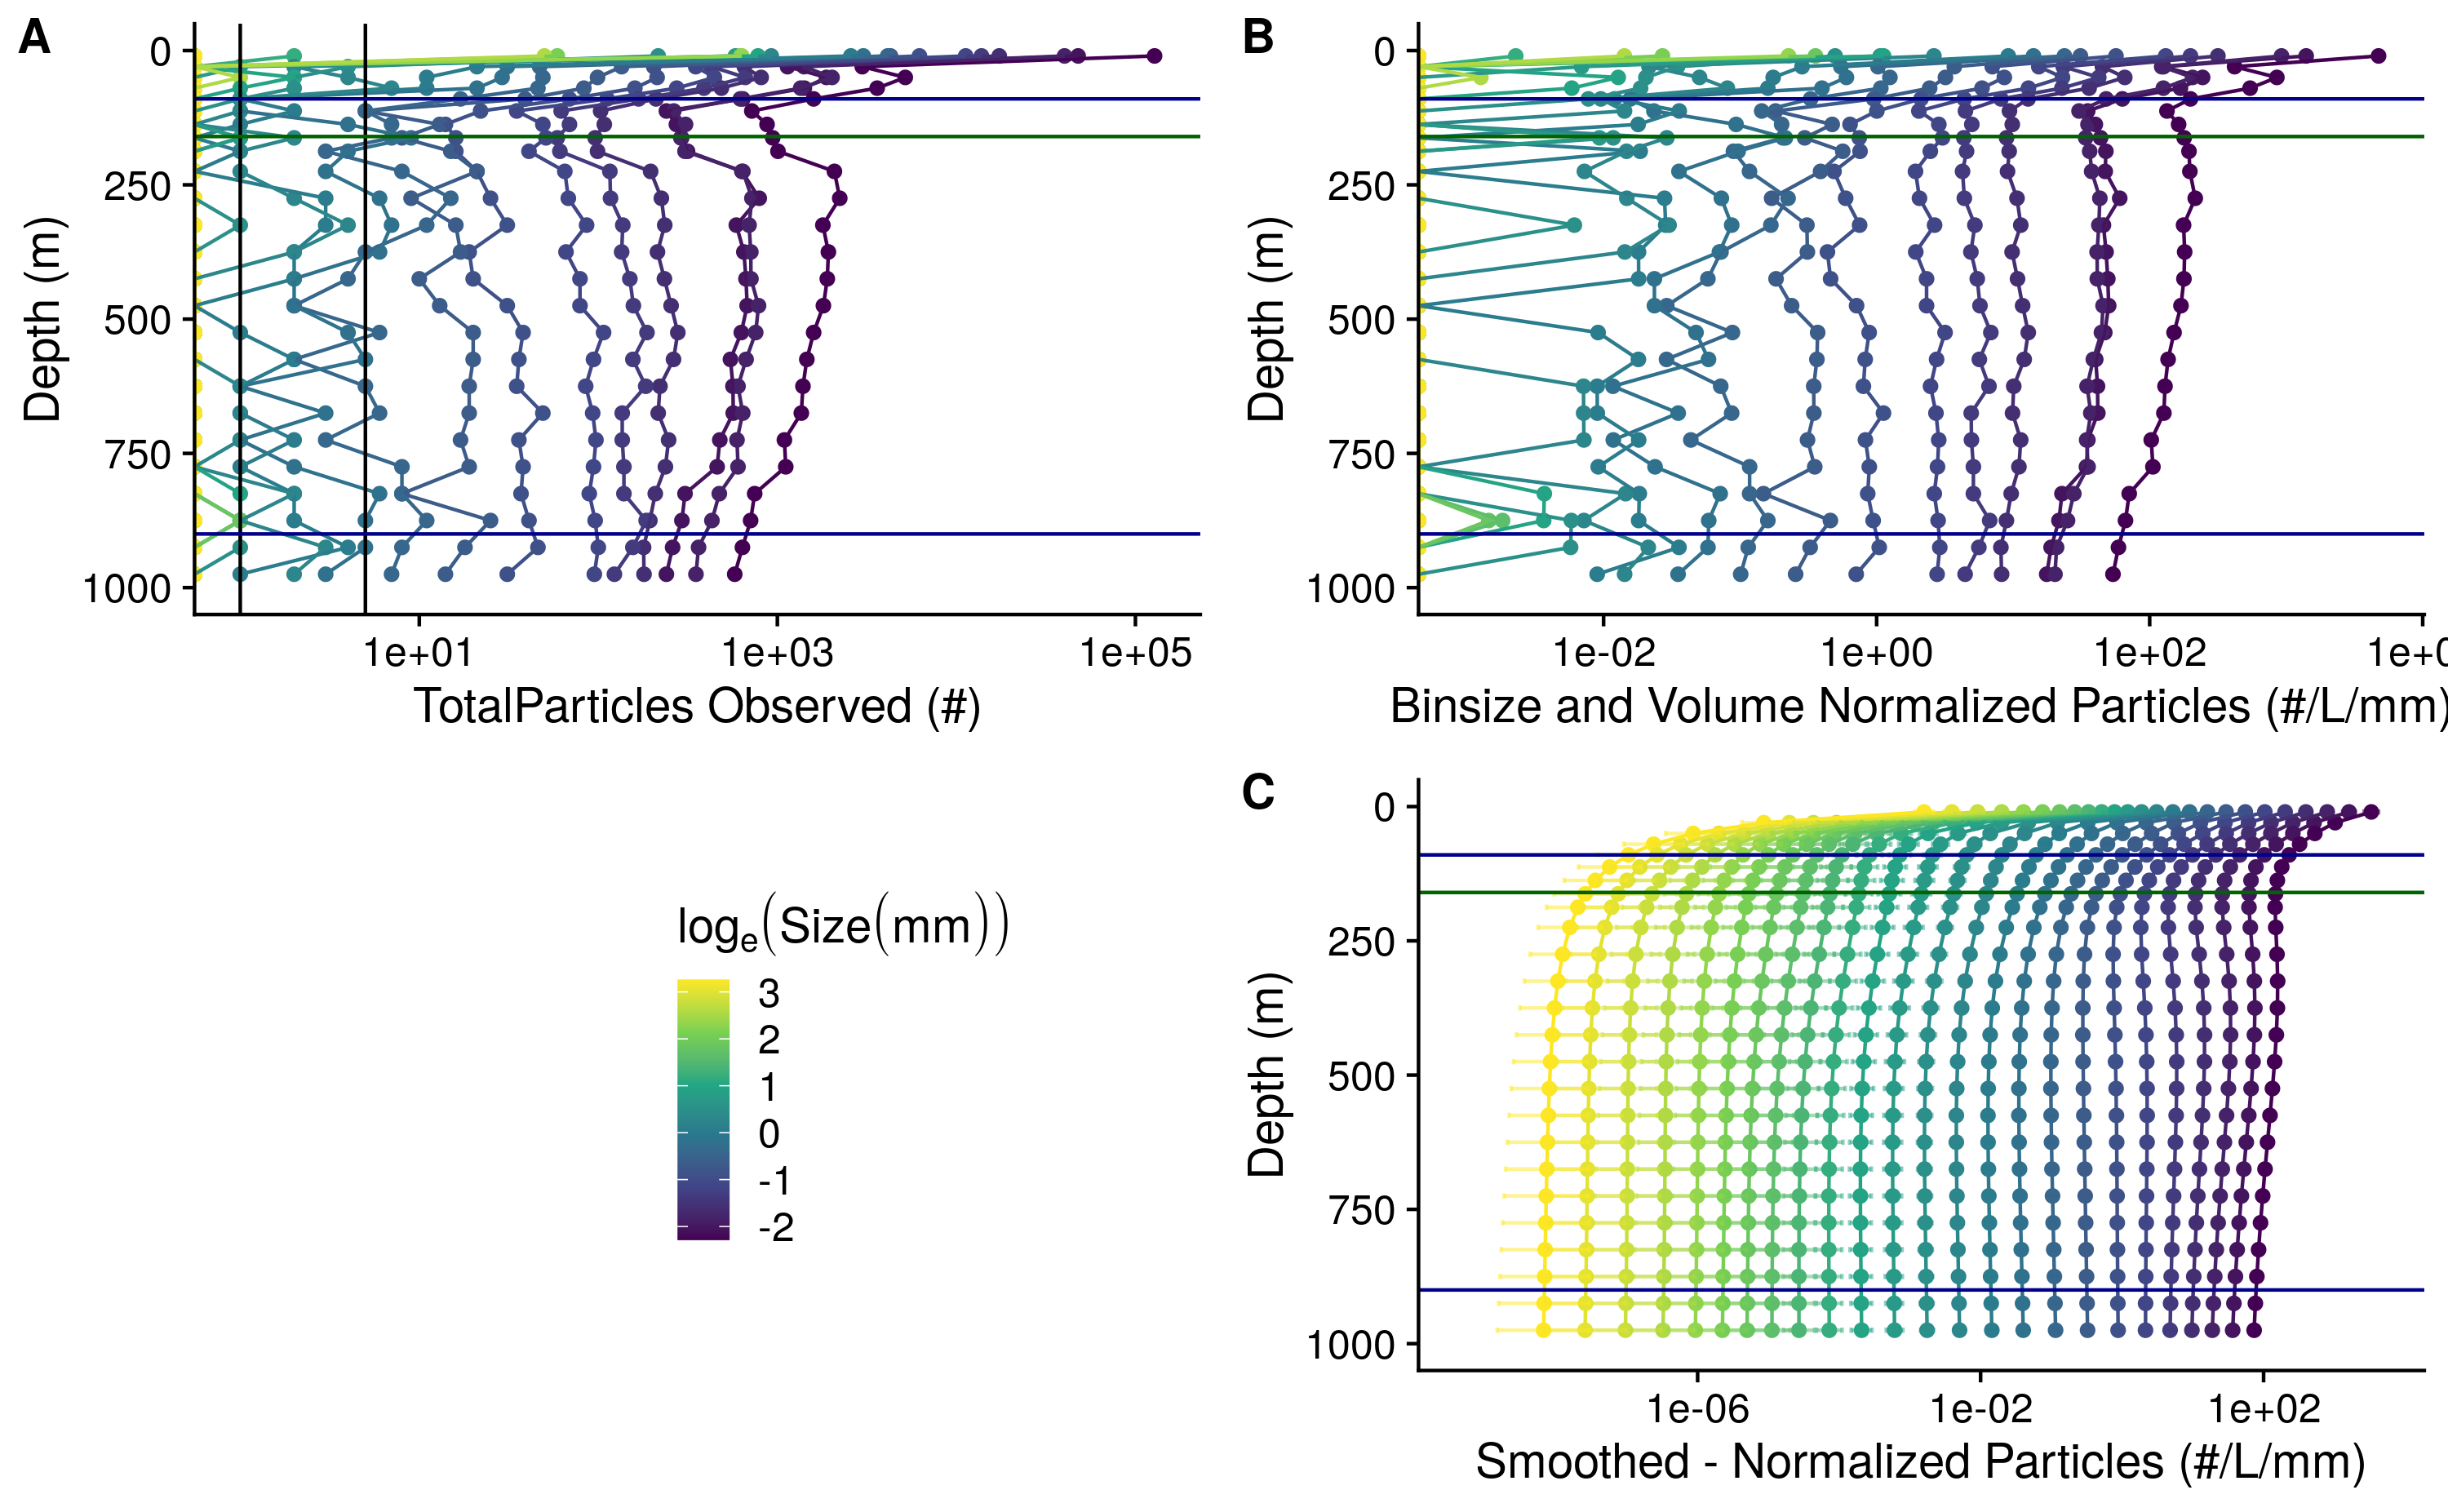
\includegraphics{../figures/AllParticleSizes.png}

Figure S4. A profile of particle abundances at different sizes and
depths. \textbf{(A)} Numbers of observed particles and \textbf{(B)}
particle numbers normalized to volume sampled and particle size bin
width. \textbf{(C)} Smoothed and extrapolated particle abundances, based
on a negative binomial GAM that predicts particle abundance form size
and depth.

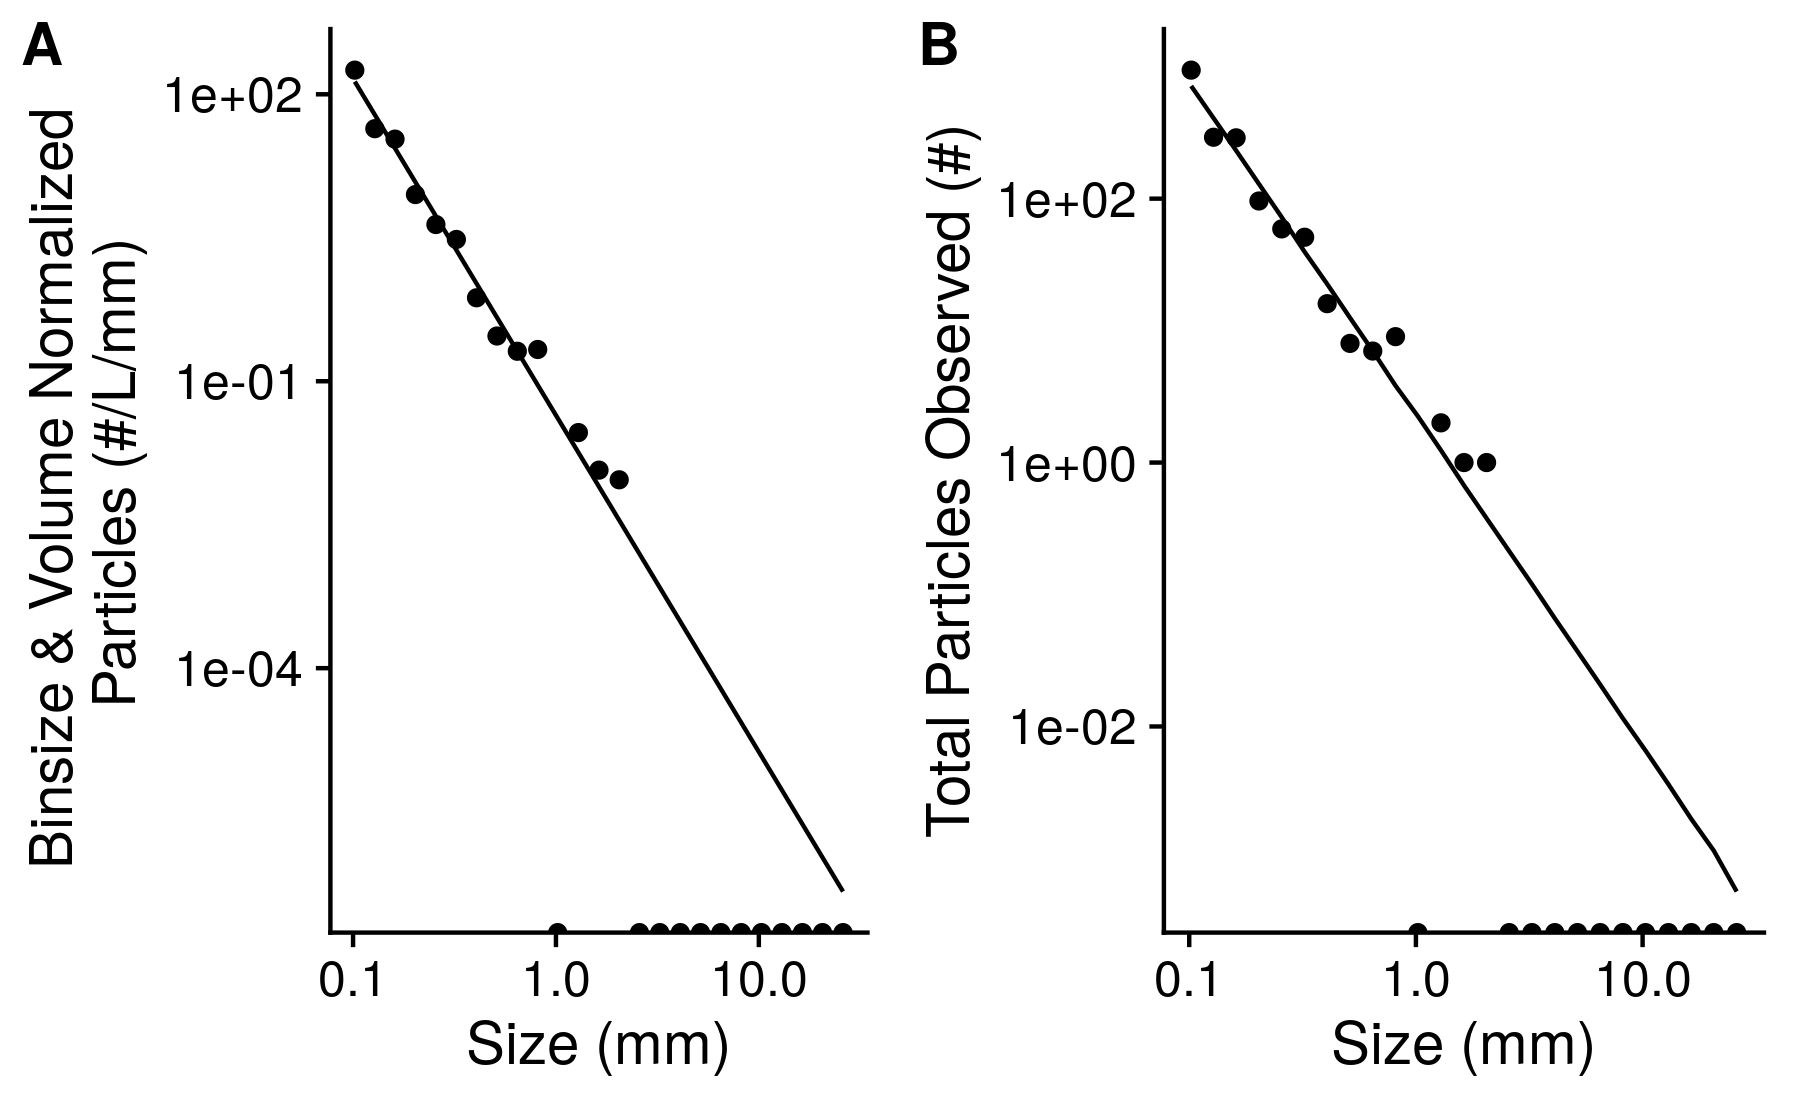
\includegraphics{../figures/ExamplePSD163m.png}

Figure S5. An example of observed particle size distribution spectra.
These are depth binned data from between X and X m deep in the water
column from the cast that occurred at \emph{DATETIME for stn\_043}. A
total volume of XXX L of water are sampled herein. Points indicate
\textbf{(A)} total numbers of observed particles and \textbf{(B)}
particle numbers normalized to volume sampled and particle size bin
width. The line indicates the predicted best fit line of the data. The
line was fit on the bin and volume normalized data by a
negative-binomial general linear model. The line in panel \textbf{A}
indicates predictions from this same model, re-scaled into absolute
particle space.

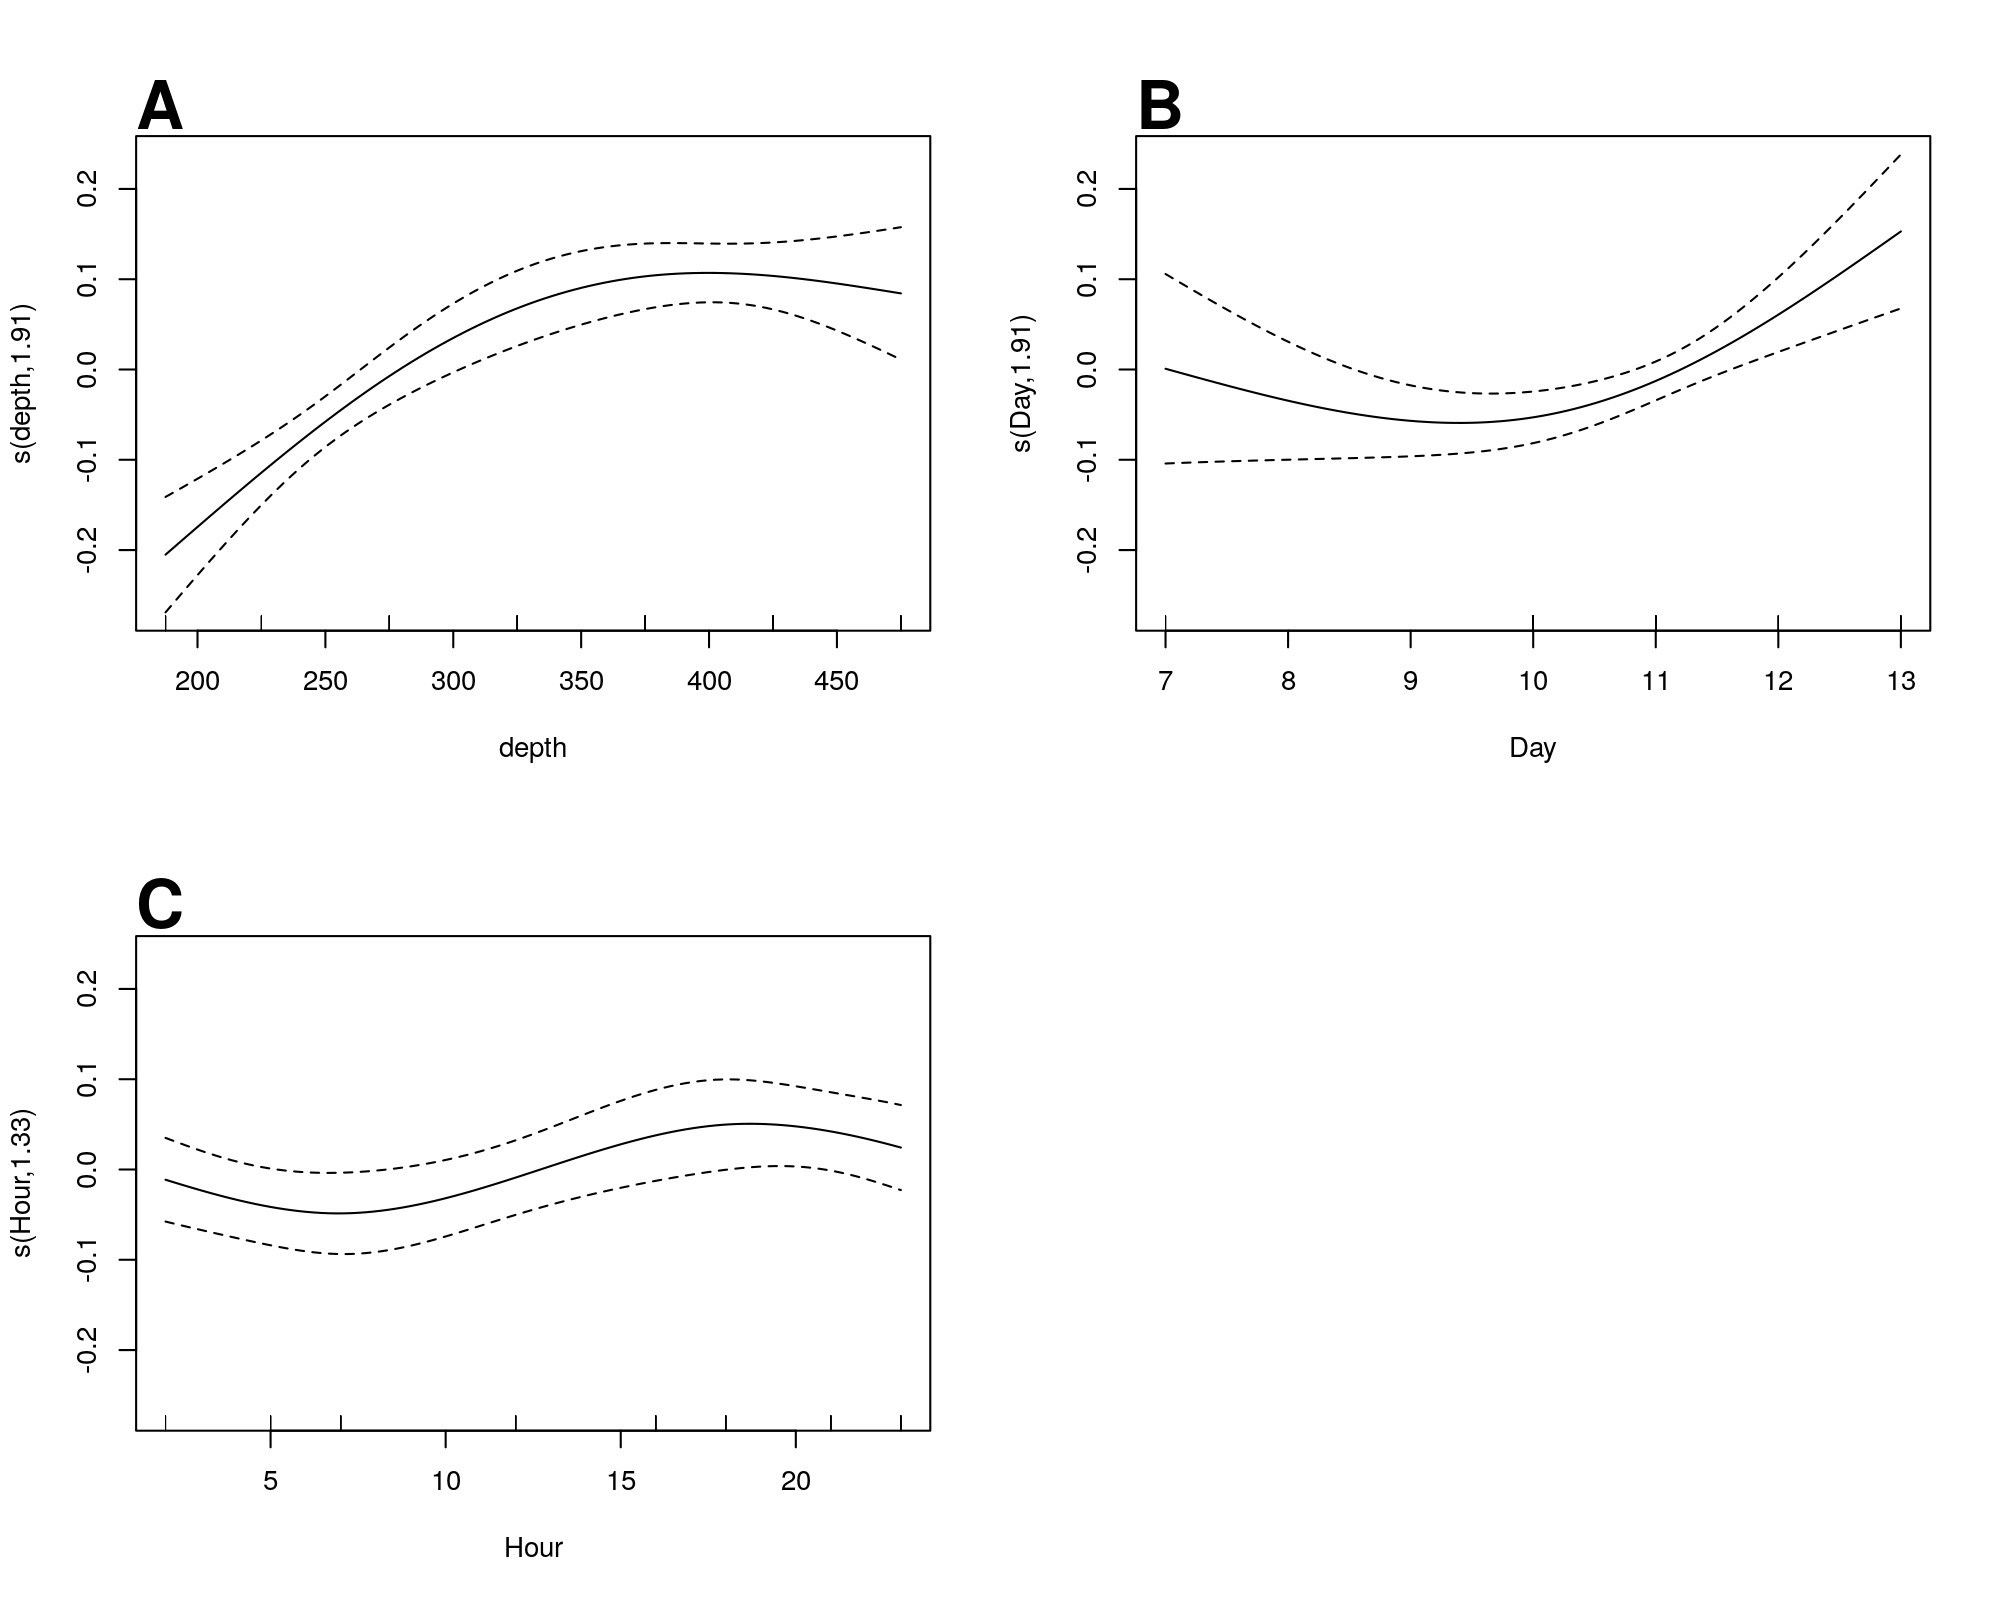
\includegraphics{../figures/FluxGamPlot.png}

Figure S6. GAM predicted effects of \textbf{A} Depth, \textbf{B} Day of
the month in January 2017, and \textbf{C} hour of the day on the
fifth-root transformed, depth normalized, rate of change of flux. Y axis
indicates the value of the component smooth functions effect on Flux.
Positive values associate with times and regions of the water column
where flux is increasing, holding other factors constant, and negative
ones where it is decreasing.

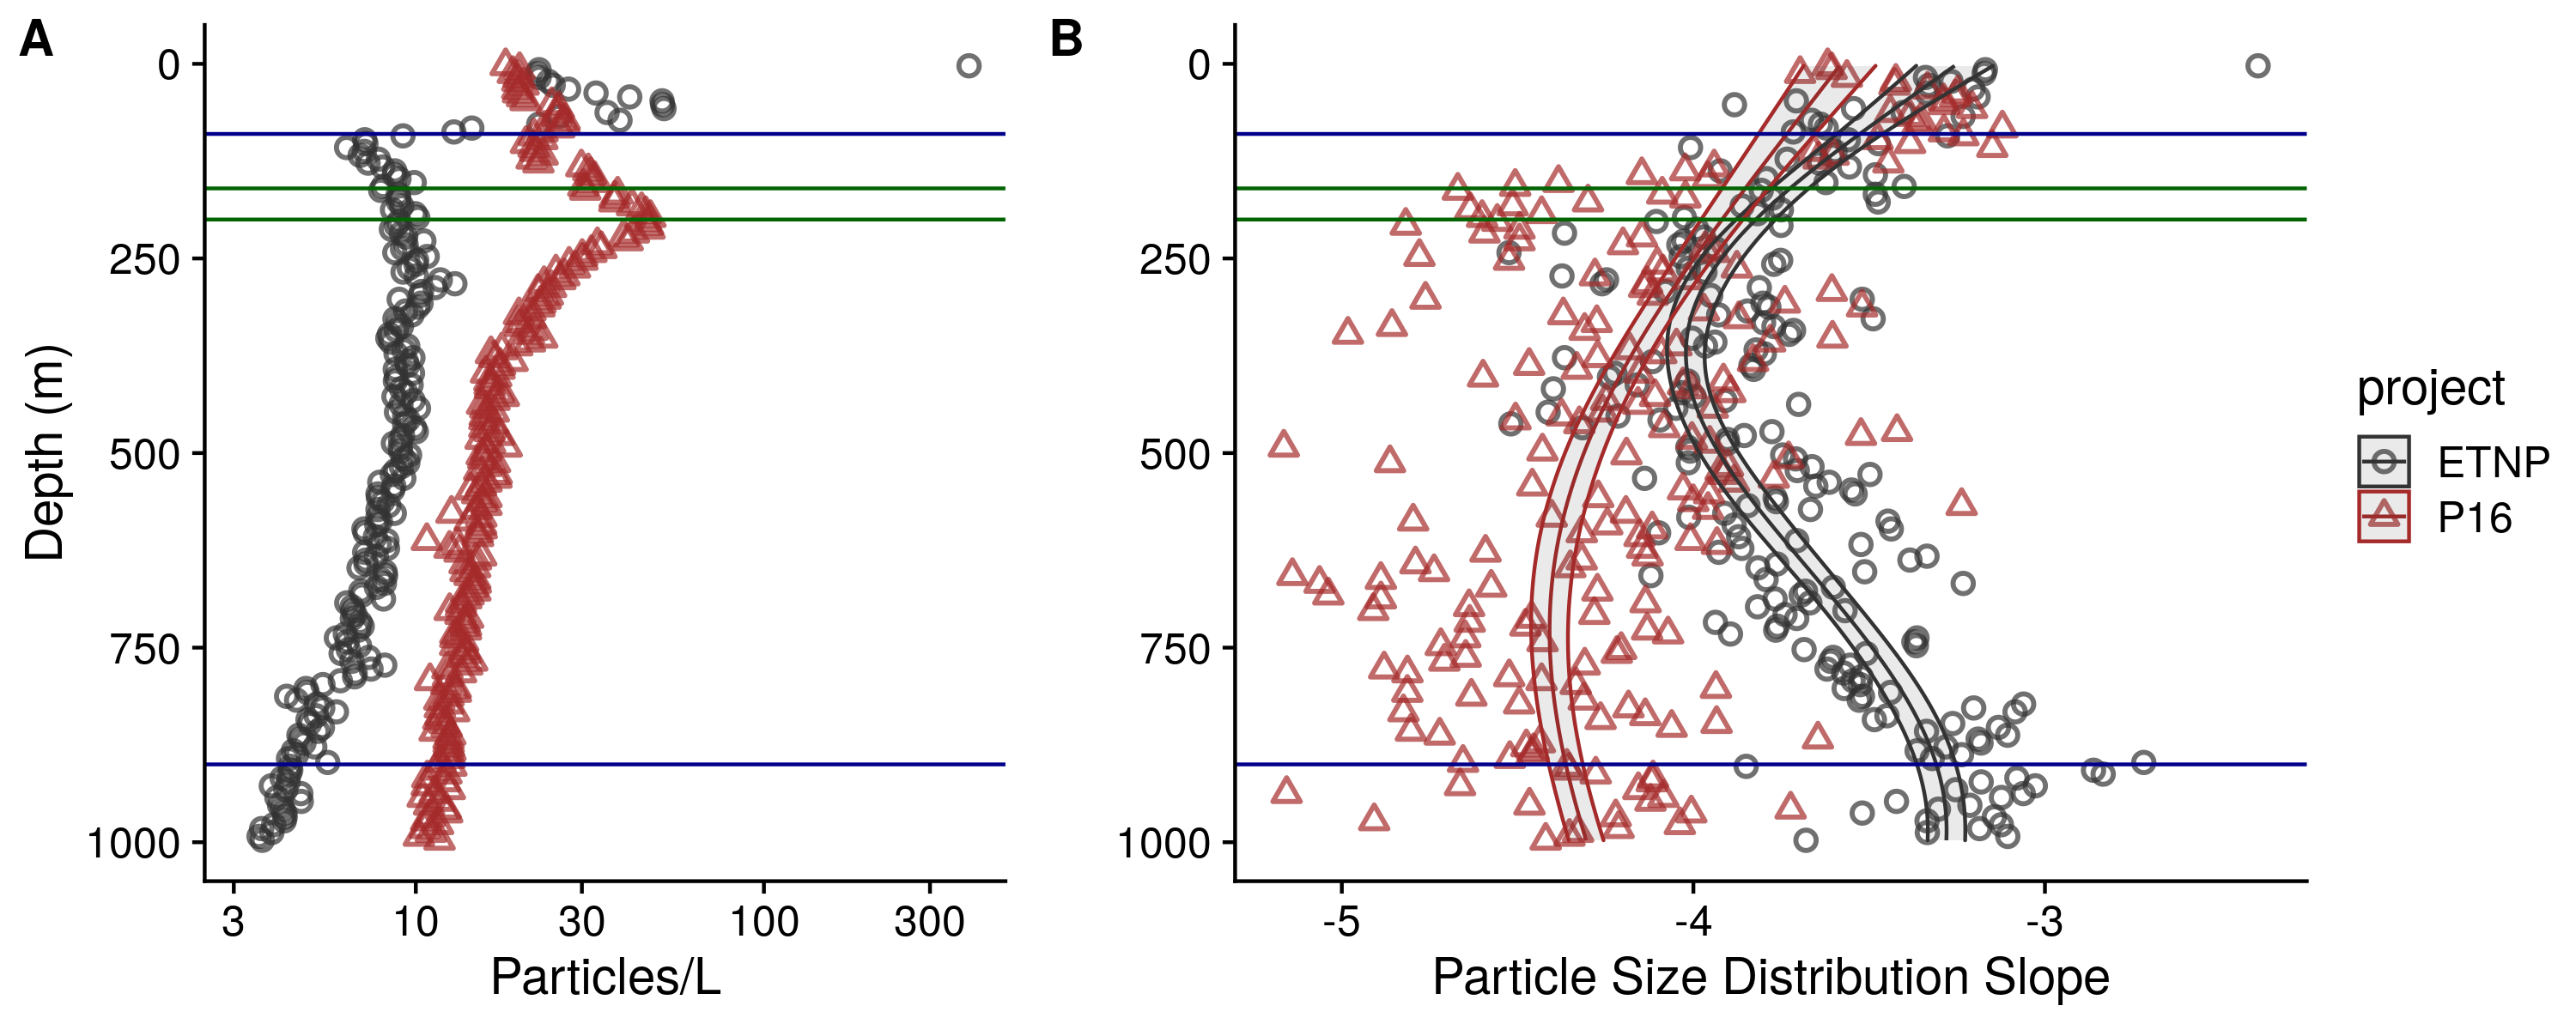
\includegraphics{../figures/ParticlesAndPSD_ETNPVsP16.png} Figure S7. As
above, but for the final cast taken at ETNP station P2 and the only cast
collected from the P16 transect at the station 100. P16 Station 100 was
chosen because it is at a similar latitude to ETNP station P2. (A) Total
particle numbers, (B) Particle size distribution. \textbf{\{Cut to
1000m\}}

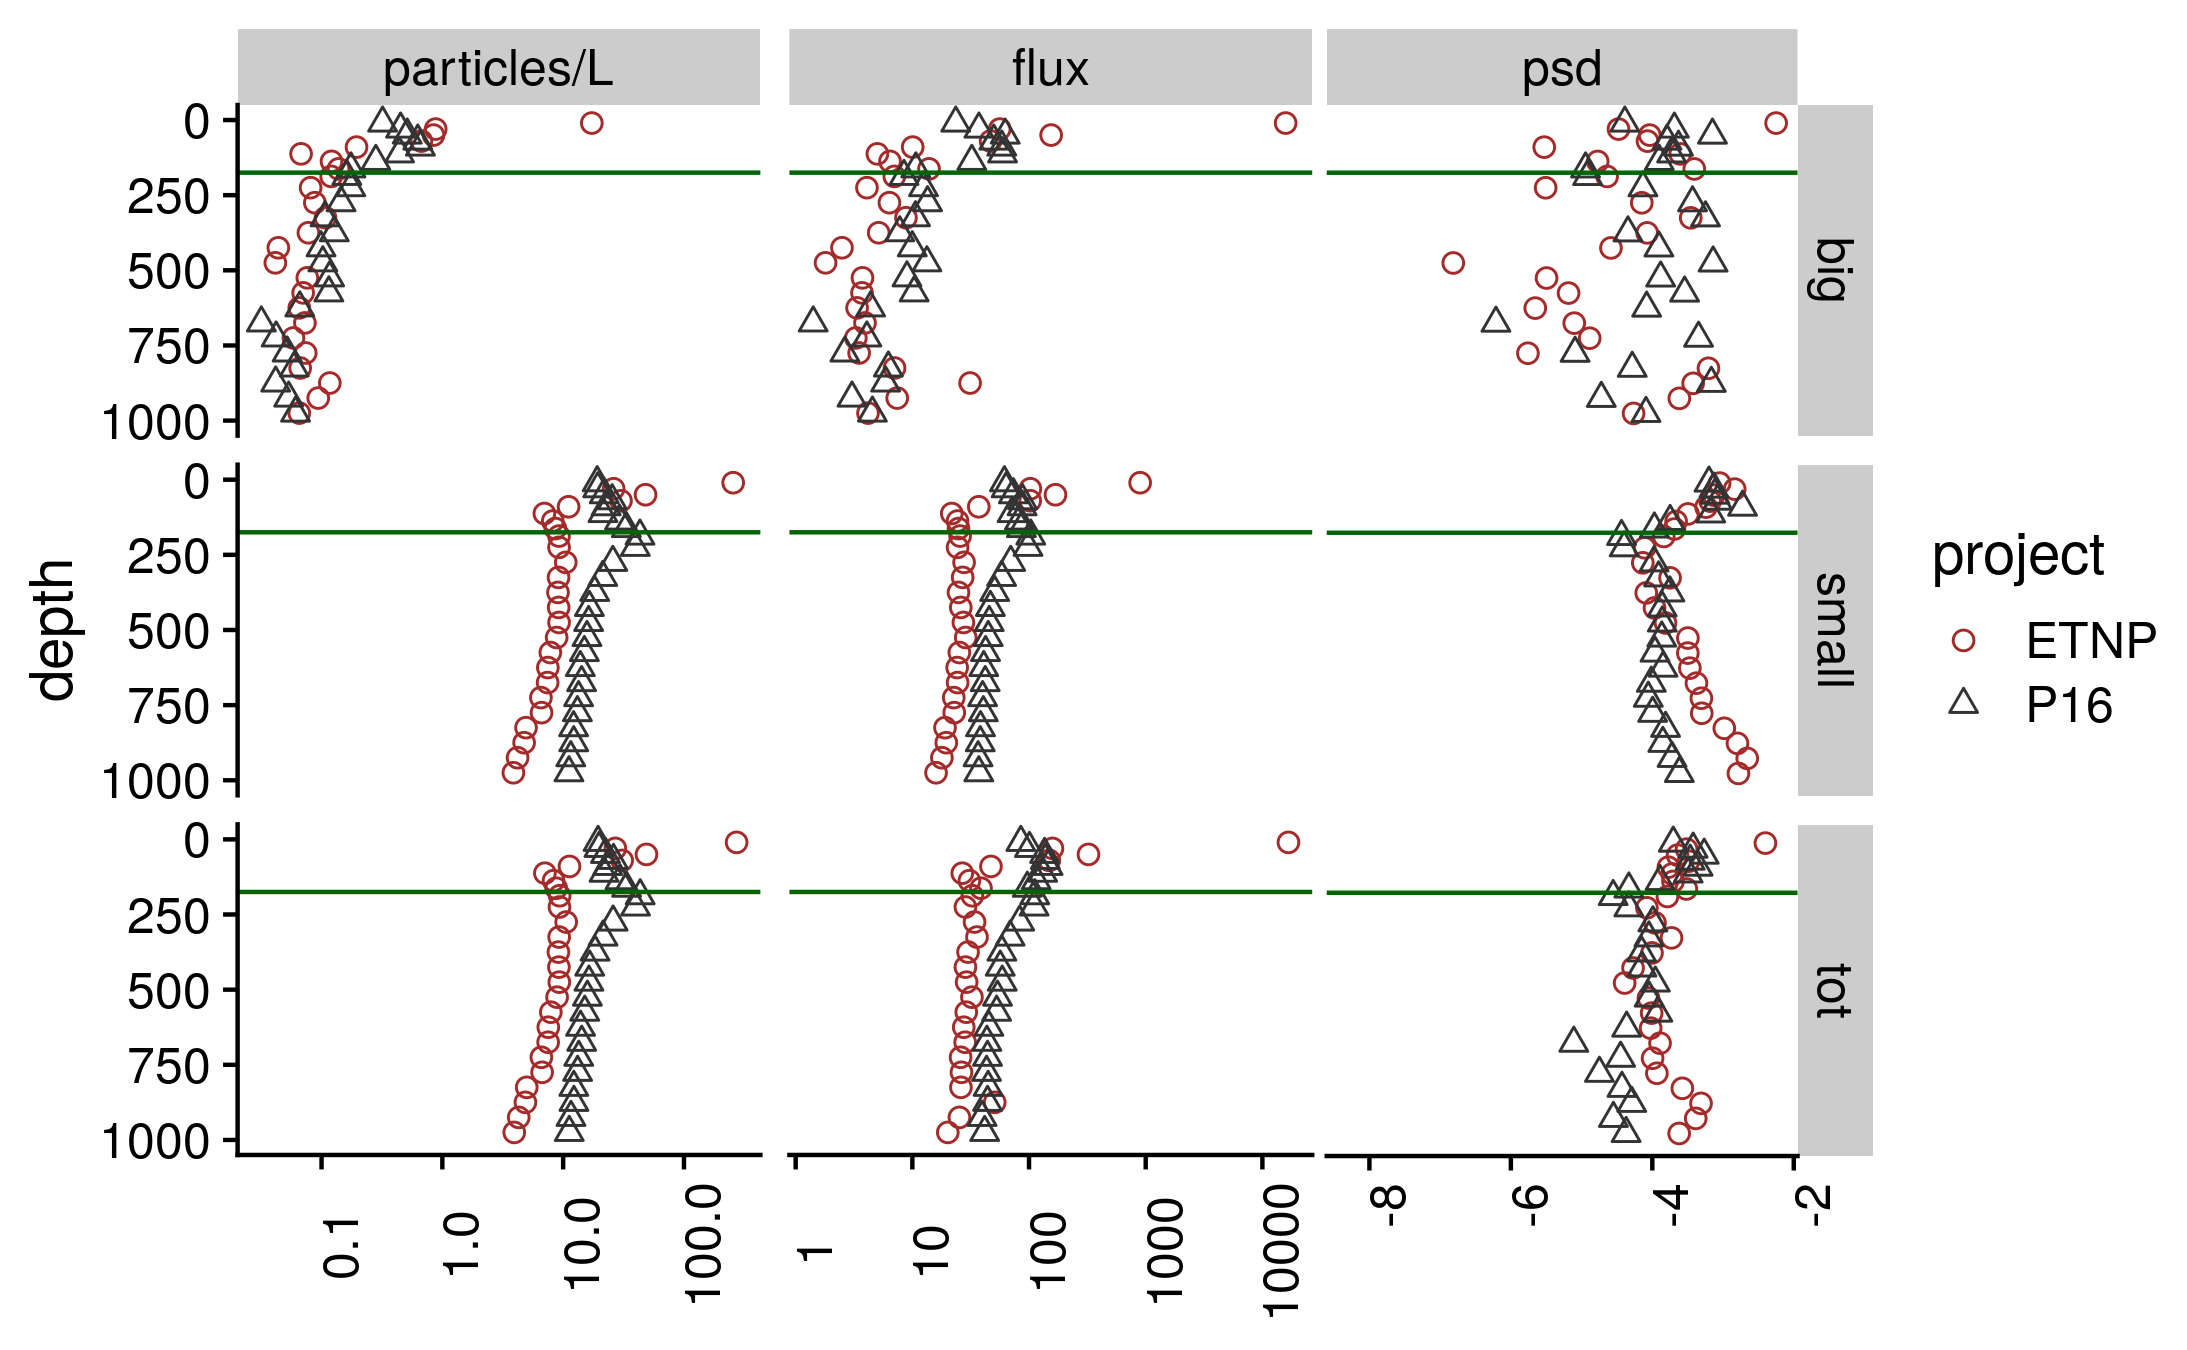
\includegraphics{../figures/BigVsSmall.png} Figure S8. Depth binned
particle number (volume normalized), particle size slope (PSD), and flux
(estimated as in Fig. 4) for large (\(>= 500\, \mu m\)), small
(\(< 500 \, \mu m\)) and total particles, at the oxic and anoxic site

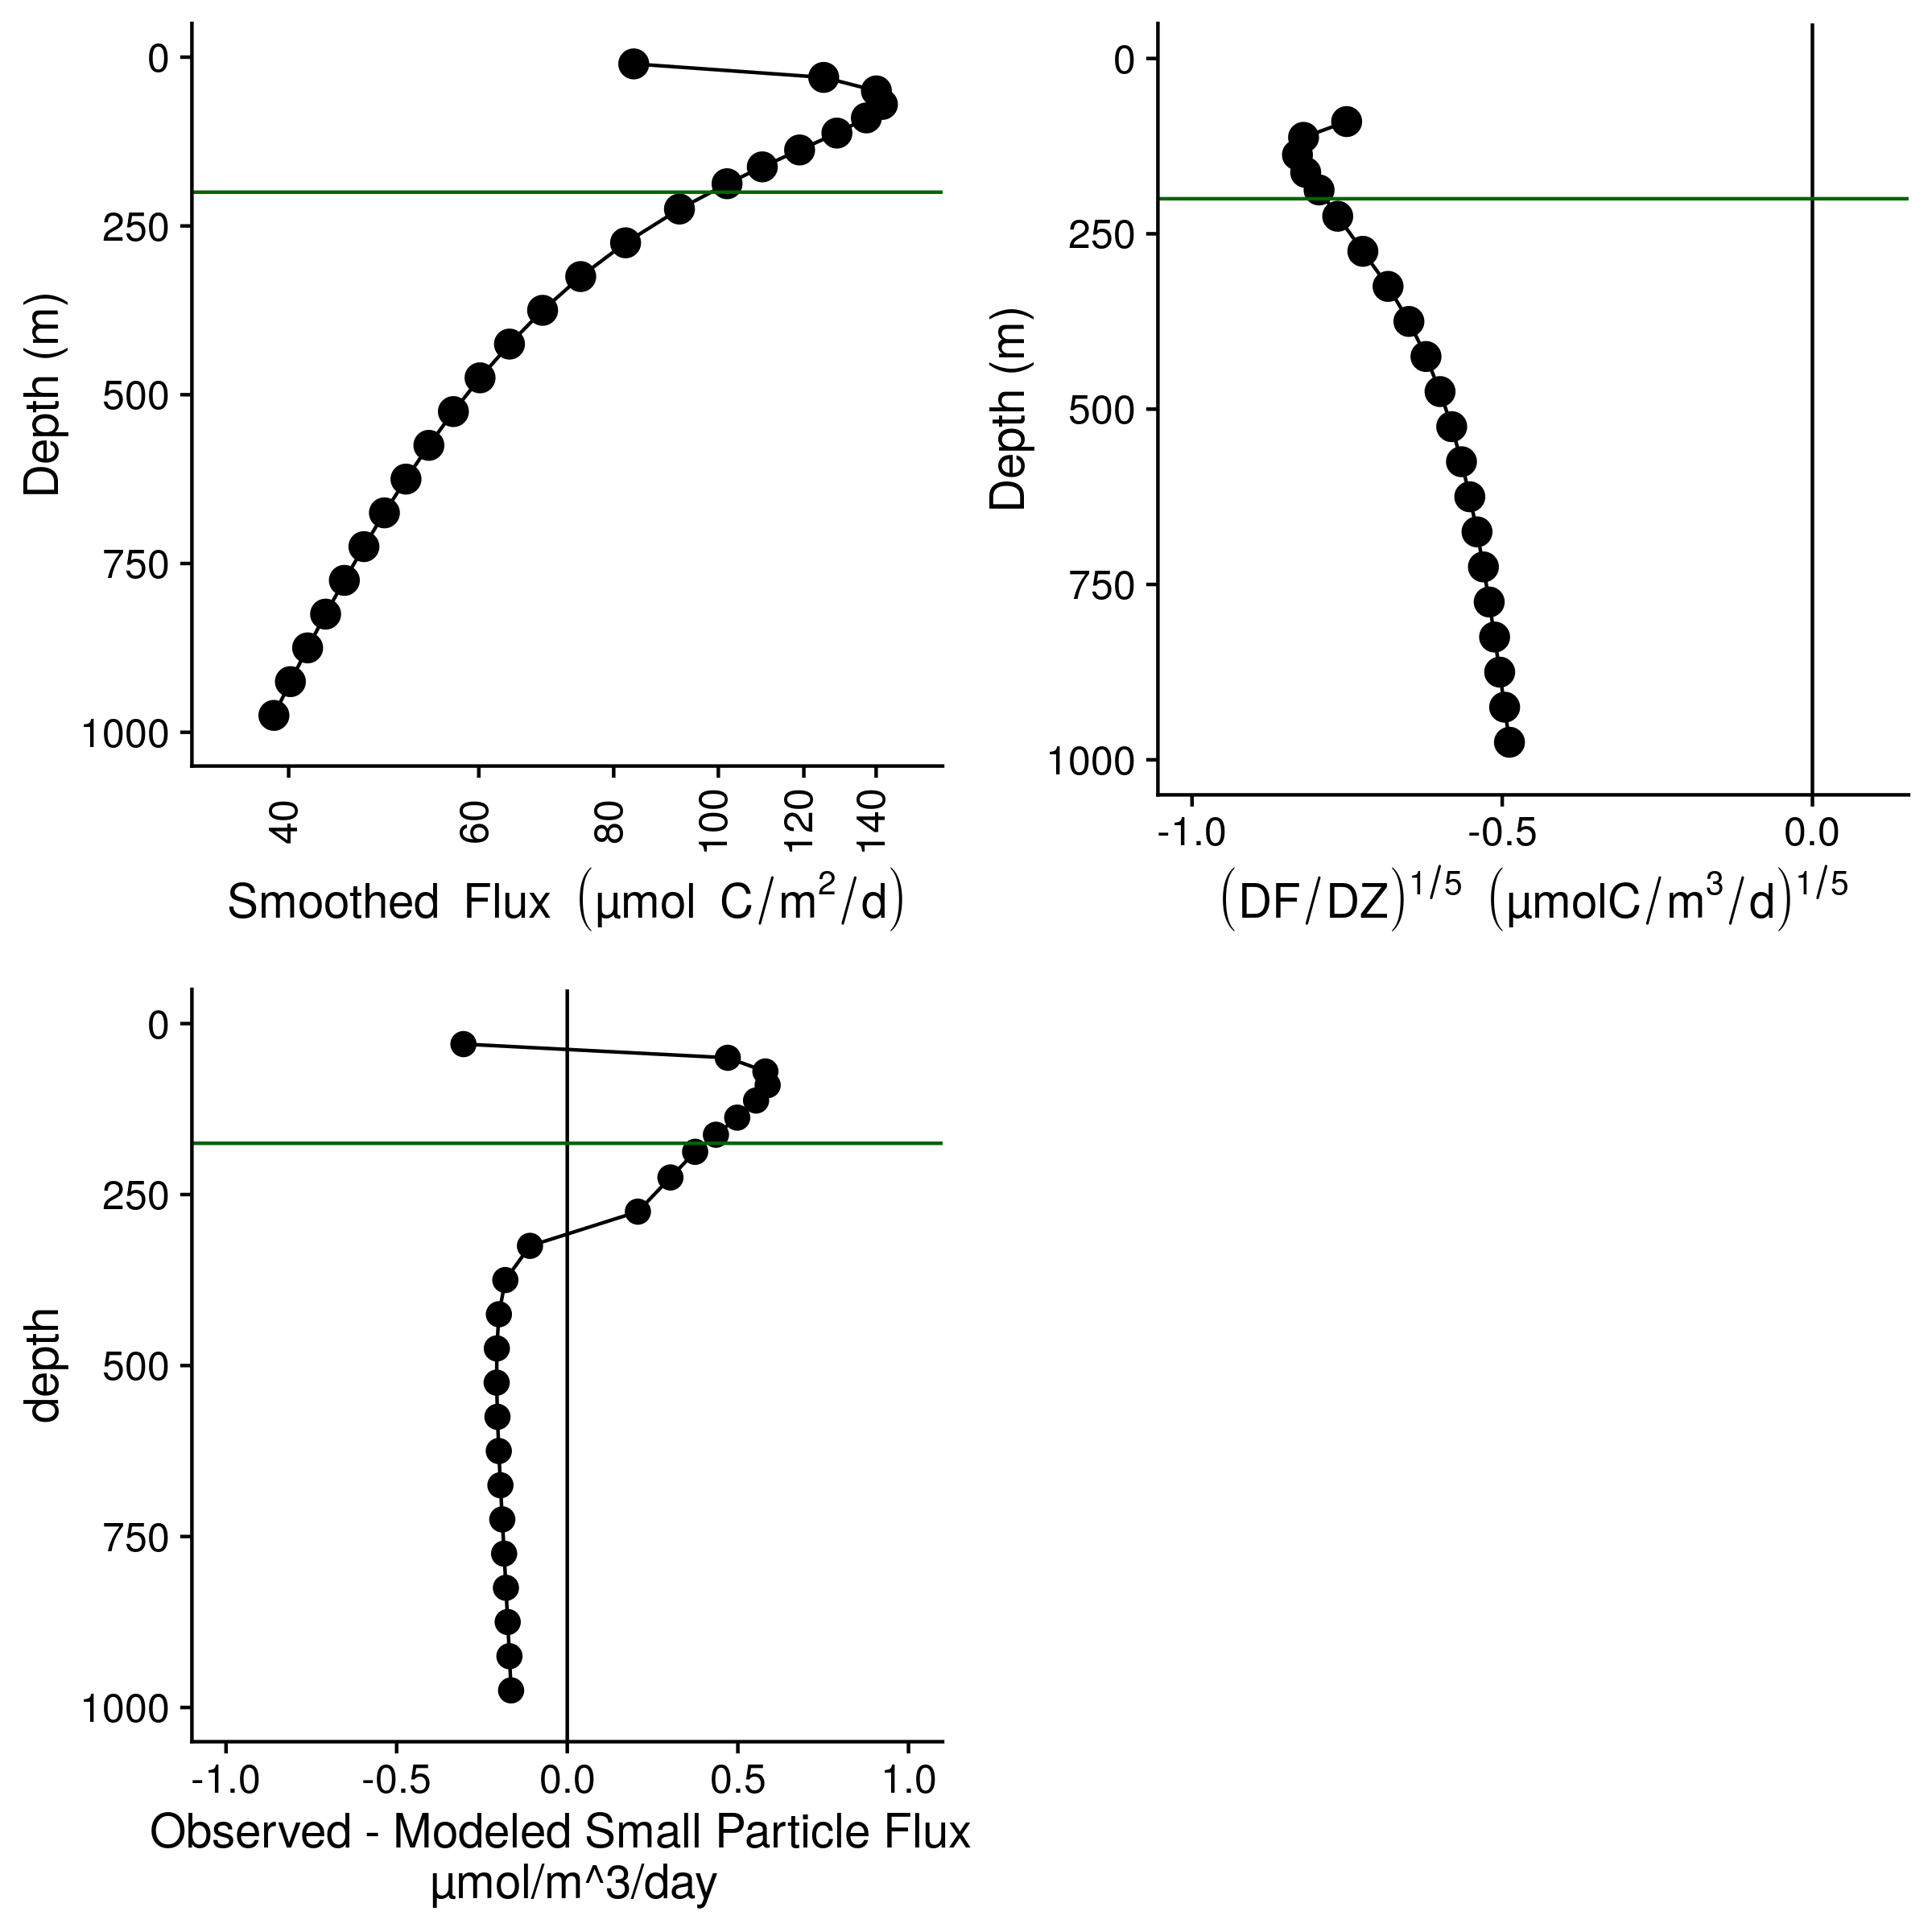
\includegraphics{../figures/P16FluxRelate.png} Figure S9. Flux profiles
and flux attenuation at P2 Station 100. \textbf{(A)} Flux profile
\textbf{(B)} Fifth-root transformed depth normalized rate of flux
decrease. \textbf{(C)} Difference between observed and modeled results.
Higher values suggest more disaggregation-like processes.

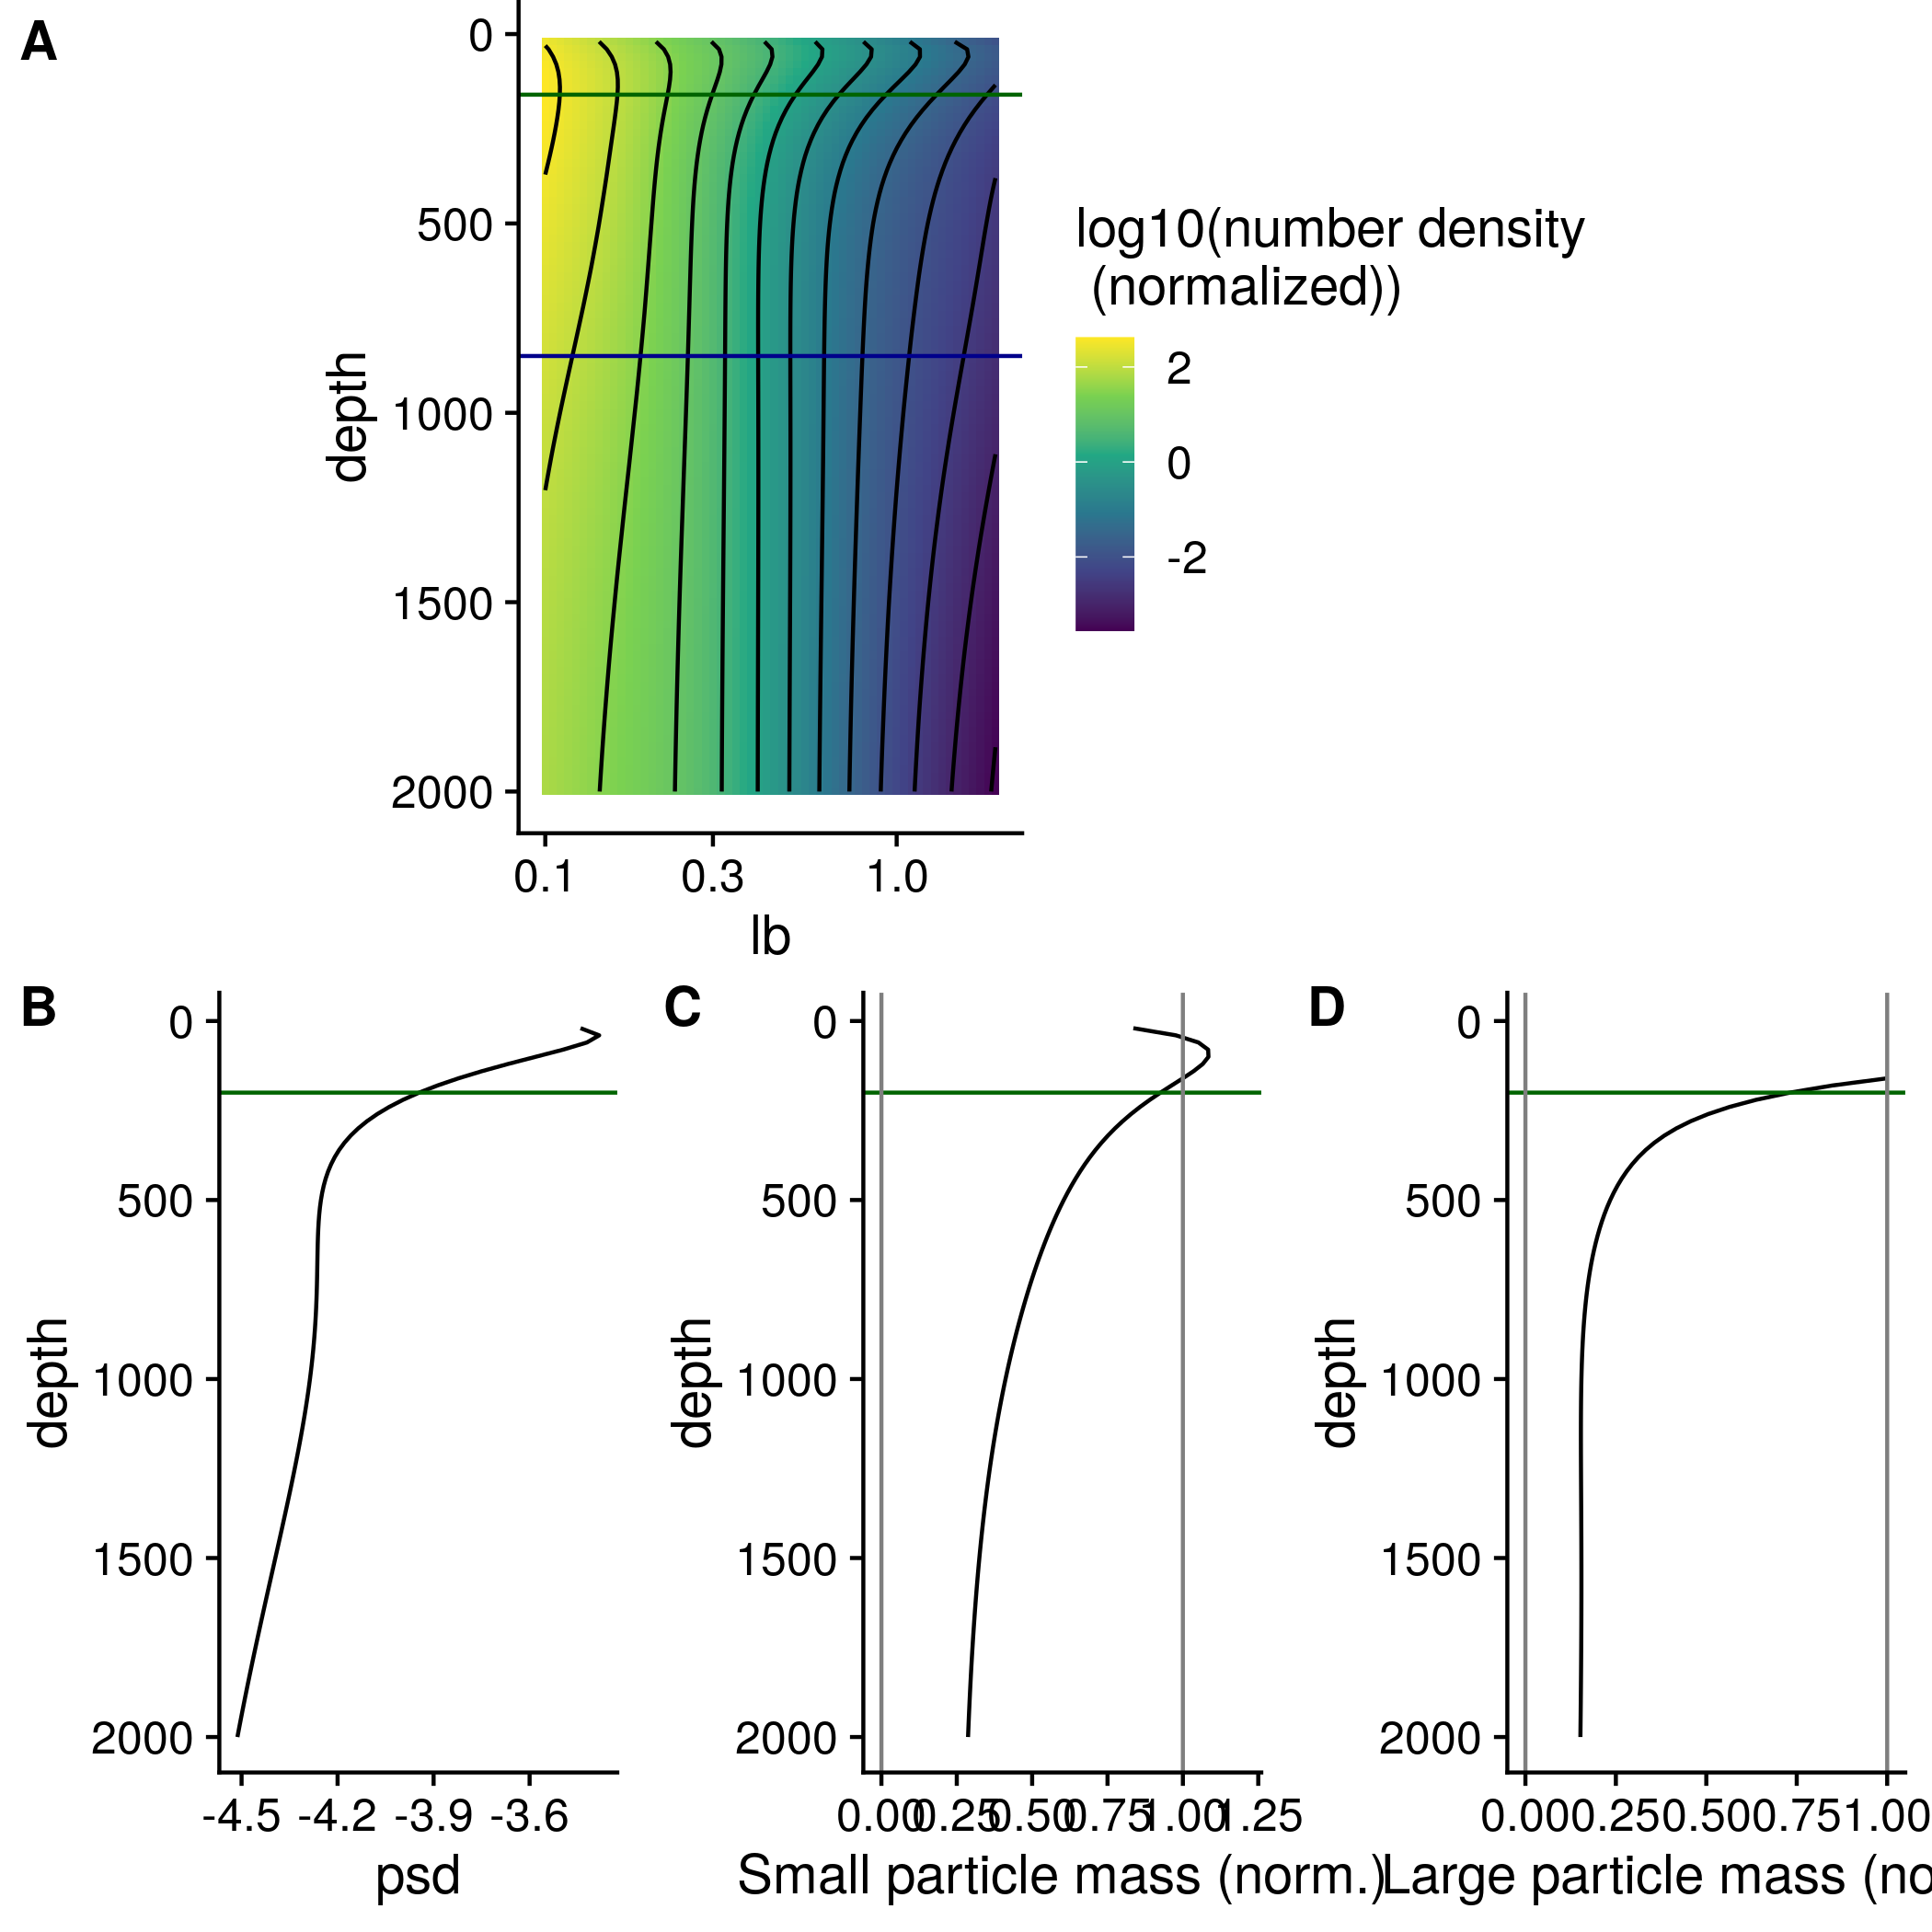
\includegraphics{../figures/WBModelValidation_Oxic.png} Figure S10. The
same profiles as shown in Figure 5, but for the oxic site P16 Station
100. \textbf{(A)} GAM smoothed bin-size and volume particle numbers at
each particle size class. \textbf{(B)} Particle size distributions. And
estimated biomass of \textbf{(C)} Small and \textbf{(D)} Large
particles.

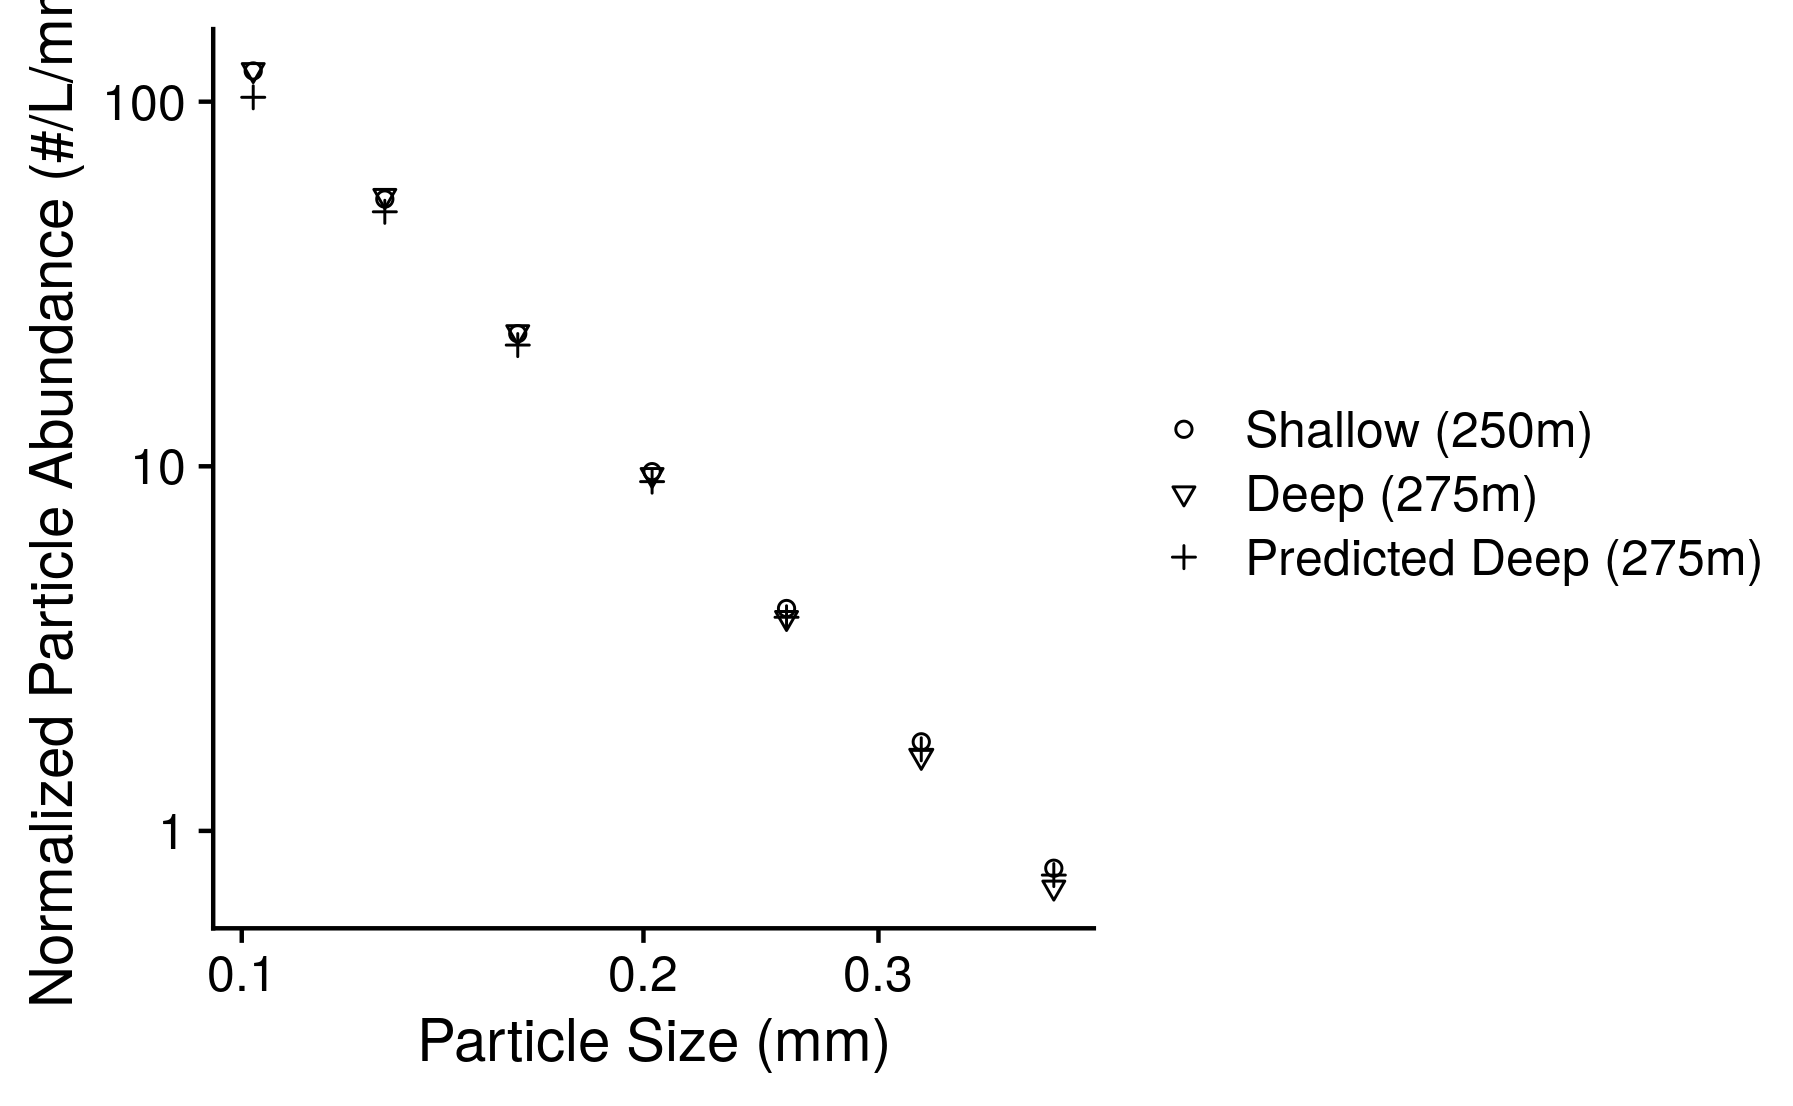
\includegraphics{../figures/DisagExample.png}

Figure S11. An example of differences between modeled and observed
particle slope. The particle size distribution at a shallow and deeper
depth are shown. The model generates a prediction of the deep depth
profile form the shallow depth profile and the flux attenuation between
the two profiles. The model predicts more attenuation of the smallest
particles than it actually observed. In practice the model compares
depths that are closer together than the two shown here. Two depths that
are far apart are shown so that the flux attenuation is large enough to
be seen by eye and to provide a conceptual example of the models'
function.

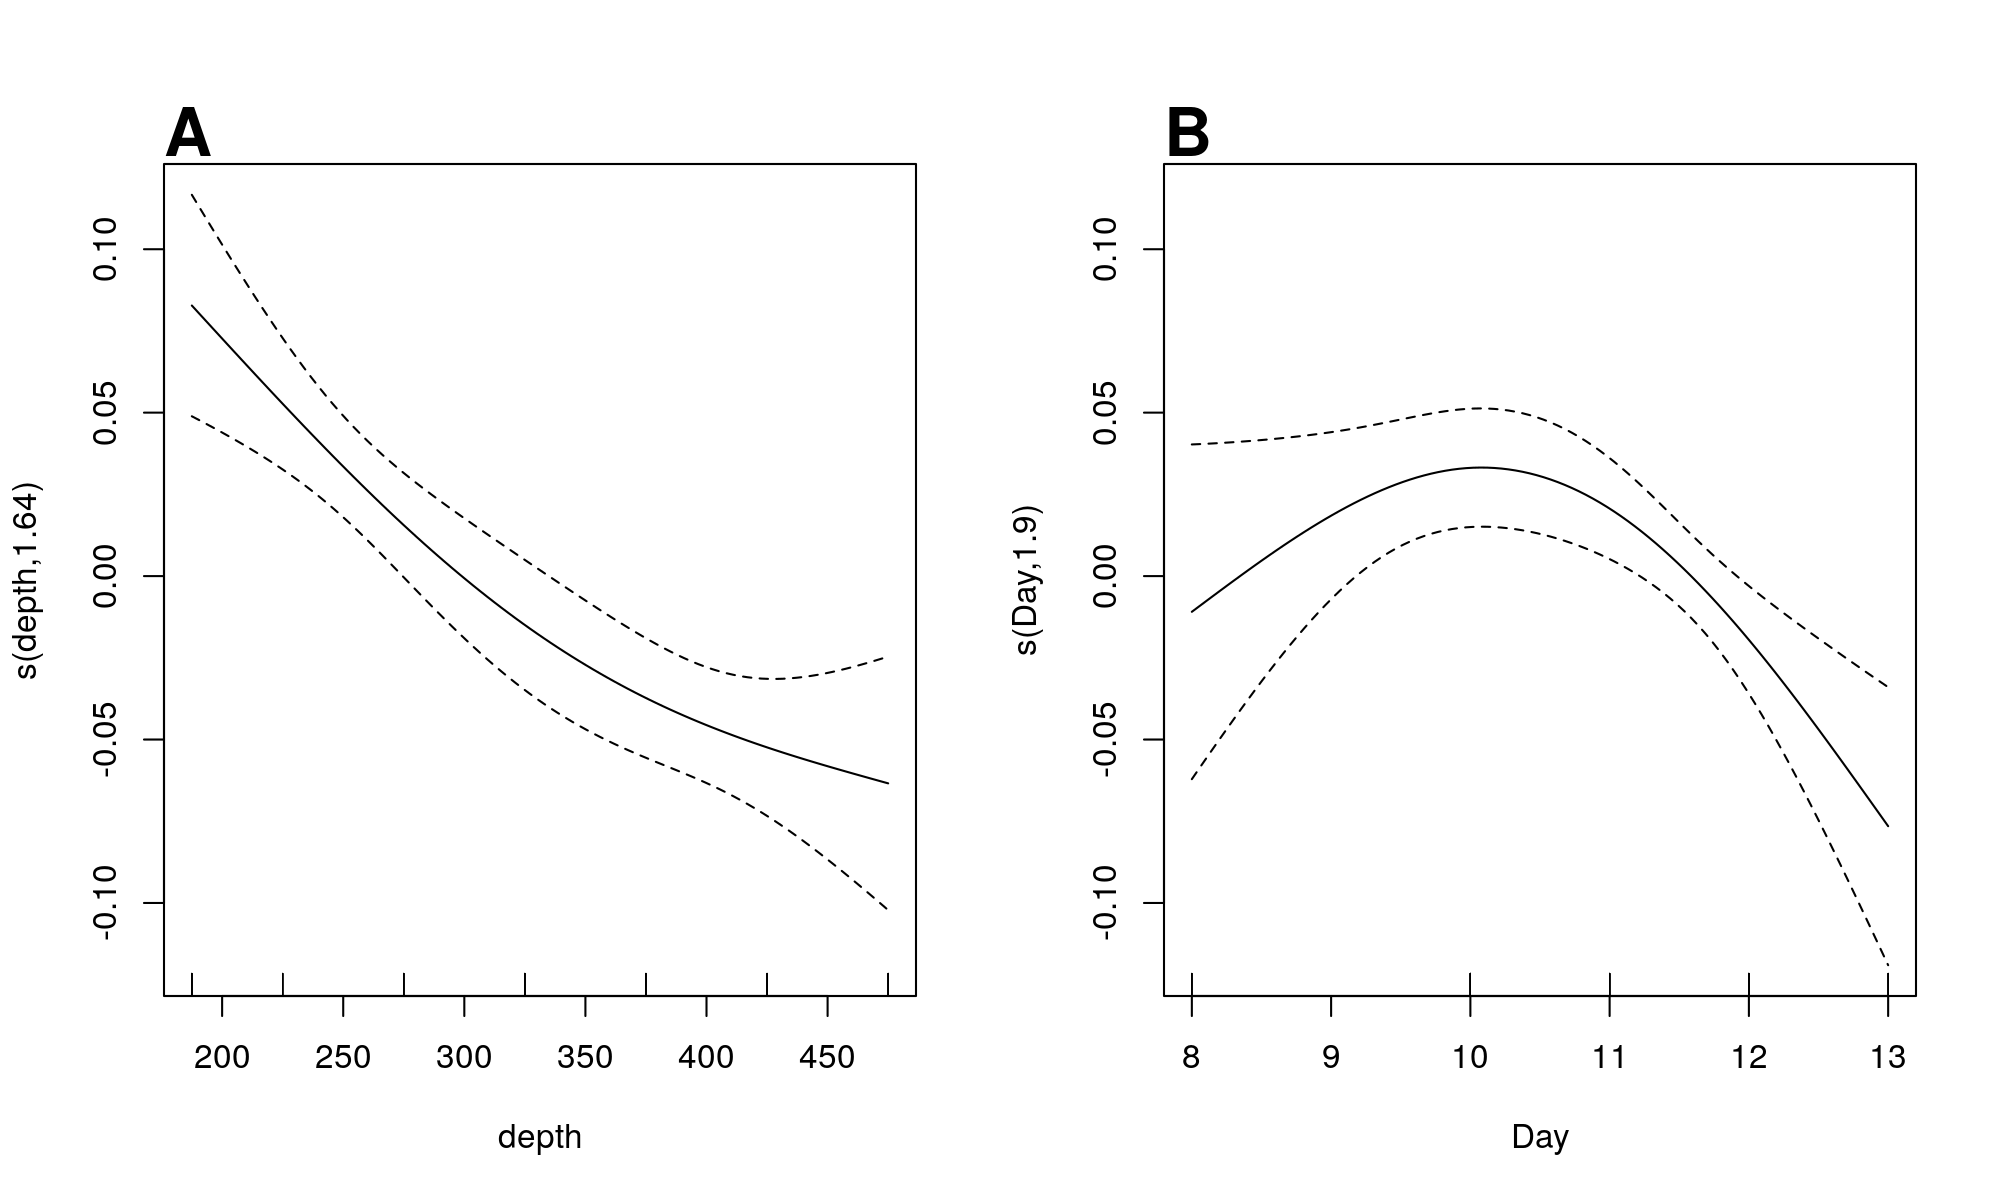
\includegraphics{../figures/OSMSGamPlot.png}

Figure S12. GAM predicted effects of \textbf{A} Depth, \textbf{B} Day of
the month in January 2017 Y axis indicates the value of the component
smooth functions effect on the difference between observed and modeled
flux. Thus higher values correspond with greater flux of small particles
than predicted by the model.

\hypertarget{cover-letter}{%
\section{Cover Letter}\label{cover-letter}}

Dear Editor,

We present for your consideration, our manuscript entitled Particle size
and abundance measurements suggest temporally variable biotic transport
and disaggregation in the Eastern Tropical North Pacific Oxygen Minimum
Zone. This manuscript presents a time-series of measurements of particle
size and abundance in the Eatern Tropical North Pacific Oxygen Deficient
zone. Our particle size measurements are complemented by the first set
of trap based measurements of carbon flux taken in the oligotrophic
section of the ETNP-OMZ and acoustic measurements of zooplankton
abundances.

Oxygen deficient zones have the capacity to regulate the global carbon
cycle, because carbon flux attenuates more slowly in the mesopelagic
when those waters are anoxic. However there is some uncertainty about
why carbon flux attenuation is so low in this region. Our measurements
support the predictions of models that suggest that all particles are
consumed more slowly by bacteria in OMZs. In contrast, they do not
conform to the predictions models that suggest that zooplankton activity
is supressed in OMZs, or that only large particles break down slowly.
Furthermore, by comparing our observations to the predictions of another
model, we provide a depth resolved estimate of the rate at which
zooplankton disaggregate large particles into smaller ones. It appears
that this apparent disaggregation is highest where acoustic data suggest
abundant zooplankton. By examining day to day variability, we also show
that the patterns that we observe are representative of conditions in
the core.

We think this manuscript will be of interest to readers of GBC because
it settles some important questions about how oxygen minimum zones
regulate the carbon cycle. In particular it presents evidence that
microbial breakdown of particles is slow in this region, even though
there are abundant electron acceptors in the form of nitrate and
nitrite, and that zooplankton still play an important role in particle
transport and breakdown, even though there is not oxygen for them to
breathe in this region.

Sincerely,

Jacob Cram

({\textbf{???}})

\hypertarget{suggested-reviewers}{%
\section{Suggested Reviewers}\label{suggested-reviewers}}

{[}co-authors, please add your favorites, we need at least 3{]}. Rainer
Kiko

\hypertarget{references}{%
\section*{References}\label{references}}
\addcontentsline{toc}{section}{References}

\hypertarget{refs}{}
\leavevmode\hypertarget{ref-andersenNewSimradEK602001}{}%
Andersen, Lars Nonboe. 2001. ``The New Simrad EK60 Scientific Echo
Sounder System.'' \emph{The Journal of the Acoustical Society of
America} 109 (5). Acoustical Society of America: 2336--6.
\url{https://doi.org/10.1121/1.4744207}.

\leavevmode\hypertarget{ref-antezanaSpeciesspecificPatternsDiel2009}{}%
Antezana, Tarsicio. 2009. ``Species-Specific Patterns of Diel Migration
into the Oxygen Minimum Zone by Euphausiids in the Humboldt Current
Ecosystem.'' \emph{Progress in Oceanography}, Eastern Boundary Upwelling
Ecosystems: Integrative and Comparative Approaches, 83 (1): 228--36.
\url{https://doi.org/10.1016/j.pocean.2009.07.039}.

\leavevmode\hypertarget{ref-archibaldModelingImpactZooplankton2019}{}%
Archibald, Kevin M., David A. Siegel, and Scott C. Doney. 2019.
``Modeling the Impact of Zooplankton Diel Vertical Migration on the
Carbon Export Flux of the Biological Pump.'' \emph{Global Biogeochemical
Cycles} 33 (2): 181--99. \url{https://doi.org/10.1029/2018GB005983}.

\leavevmode\hypertarget{ref-bianchiIntensificationOpenoceanOxygen2013}{}%
Bianchi, Daniele, Eric D. Galbraith, David A. Carozza, K. a. S. Mislan,
and Charles A. Stock. 2013. ``Intensification of Open-Ocean Oxygen
Depletion by Vertically Migrating Animals.'' \emph{Nature Geoscience} 6
(7). Nature Publishing Group: 545--48.
\url{https://doi.org/10.1038/ngeo1837}.

\leavevmode\hypertarget{ref-bianchiGlobalNicheMarine2018}{}%
Bianchi, Daniele, Thomas S. Weber, Rainer Kiko, and Curtis Deutsch.
2018. ``Global Niche of Marine Anaerobic Metabolisms Expanded by
Particle Microenvironments.'' \emph{Nature Geoscience} 11 (4). Nature
Publishing Group: 263. \url{https://doi.org/10.1038/s41561-018-0081-0}.

\leavevmode\hypertarget{ref-boyerWorldOceanAtlas2018}{}%
Boyer, T., H.E. Garcia, R.A. Locarini, A. Ricardo, M.M. Zweng, A.V
Mishonov, J.R. Reagan, et al. 2018. ``World Ocean Atlas 2018.'' NOAA
National Centers for Environmntal Information.

\leavevmode\hypertarget{ref-breitburgDecliningOxygenGlobal2018}{}%
Breitburg, Denise, Lisa A. Levin, Andreas Oschlies, Marilaure
Gr\a'egoire, Francisco P. Chavez, Daniel J. Conley, V\a'eronique Garçon,
et al. 2018. ``Declining Oxygen in the Global Ocean and Coastal
Waters.'' \emph{Science} 359 (6371). American Association for the
Advancement of Science. \url{https://doi.org/10.1126/science.aam7240}.

\leavevmode\hypertarget{ref-burdParticleAggregation2009}{}%
Burd, Adrian B., and George A. Jackson. 2009. ``Particle Aggregation.''
\emph{Annual Review of Marine Science} 1 (1): 65--90.
\url{https://doi.org/10.1146/annurev.marine.010908.163904}.

\leavevmode\hypertarget{ref-cavanRoleZooplanktonDetermining2017}{}%
Cavan, Emma L., Stephanie A. Henson, Anna Belcher, and Richard Sanders.
2017. ``Role of Zooplankton in Determining the Efficiency of the
Biological Carbon Pump.'' \emph{Biogeosciences} 14 (January): 177--86.
\url{https://doi.org/10.5194/bg-14-177-2017}.

\leavevmode\hypertarget{ref-cisewskiSeasonalVariationDiel2010}{}%
Cisewski, Boris, Volker H. Strass, Monika Rhein, and Sören Krägefsky.
2010. ``Seasonal Variation of Diel Vertical Migration of Zooplankton
from ADCP Backscatter Time Series Data in the Lazarev Sea, Antarctica.''
\emph{Deep Sea Research Part I: Oceanographic Research Papers} 57 (1):
78--94. \url{https://doi.org/10.1016/j.dsr.2009.10.005}.

\leavevmode\hypertarget{ref-cramRoleParticleSize2018}{}%
Cram, Jacob A., Thomas Weber, Shirley W. Leung, Andrew M. P. McDonnell,
Jun-Hong Liang, and Curtis Deutsch. 2018. ``The Role of Particle Size,
Ballast, Temperature, and Oxygen in the Sinking Flux to the Deep Sea.''
\emph{Global Biogeochemical Cycles} 32 (5): 858--76.
\url{https://doi.org/10.1029/2017GB005710}.

\leavevmode\hypertarget{ref-deutschCentennialChangesNorth2014}{}%
Deutsch, C., W. Berelson, R. Thunell, T. Weber, C. Tems, J. McManus, J.
Crusius, et al. 2014. ``Centennial Changes in North Pacific Anoxia
Linked to Tropical Trade Winds.'' \emph{Science} 345 (6197): 665--68.
\url{https://doi.org/10.1126/science.1252332}.

\leavevmode\hypertarget{ref-devriesExportFateOrganic2017}{}%
DeVries, Timothy, and Thomas Weber. 2017. ``The Export and Fate of
Organic Matter in the Ocean: New Constraints from Combining Satellite
and Oceanographic Tracer Observations.'' \emph{Global Biogeochemical
Cycles}, January, 2016GB005551.
\url{https://doi.org/10.1002/2016GB005551}.

\leavevmode\hypertarget{ref-devriesMechanisticParticleFlux2014}{}%
DeVries, T., J.-H. Liang, and C. Deutsch. 2014. ``A Mechanistic Particle
Flux Model Applied to the Oceanic Phosphorus Cycle.''
\emph{Biogeosciences Discuss.} 11 (3): 3653--99.
\url{https://doi.org/10.5194/bgd-11-3653-2014}.

\leavevmode\hypertarget{ref-dillingFragmentationMarineSnow2000}{}%
Dilling, Lisa, and Alice L Alldredge. 2000. ``Fragmentation of Marine
Snow by Swimming Macrozooplankton: A New Process Impacting Carbon
Cycling in the Sea.'' \emph{Deep Sea Research Part I: Oceanographic
Research Papers} 47 (7): 1227--45.
\url{https://doi.org/10.1016/S0967-0637(99)00105-3}.

\leavevmode\hypertarget{ref-durkinObservationsCarbonExport2015}{}%
Durkin, Colleen A., Margaret L. Estapa, and Ken O. Buesseler. 2015.
``Observations of Carbon Export by Small Sinking Particles in the Upper
Mesopelagic.'' \emph{Marine Chemistry}, Particles in aquatic
environments: From invisible exopolymers to sinking aggregates, 175
(October): 72--81. \url{https://doi.org/10.1016/j.marchem.2015.02.011}.

\leavevmode\hypertarget{ref-evansRoleWaterMasses2020}{}%
Evans, Natalya, Elisabeth Boles, Jarek V. Kwiecinski, Susan Mullen,
Martin Wolf, Allan H. Devol, Rintaro Moriyasu, SungHyun Nam, Andrew R.
Babbin, and James W. Moffett. 2020. ``The Role of Water Masses in
Shaping the Distribution of Redox Active Compounds in the Eastern
Tropical North Pacific Oxygen Deficient Zone and Influencing Low Oxygen
Concentrations in the Eastern Pacific Ocean.'' \emph{Limnology and
Oceanography} 65 (8): 1688--1705.
\url{https://doi.org/10.1002/lno.11412}.

\leavevmode\hypertarget{ref-francoisFactorsControllingFlux2002}{}%
Francois, Roger, Susumu Honjo, Richard Krishfield, and Steve Manganini.
2002. ``Factors Controlling the Flux of Organic Carbon to the
Bathypelagic Zone of the Ocean.'' \emph{Global Biogeochemical Cycles} 16
(4): 34--31--34--20. \url{https://doi.org/10.1029/2001GB001722}.

\leavevmode\hypertarget{ref-fuchsmanCyanobacteriaCyanophageContributions2019}{}%
Fuchsman, Clara A., Hilary I. Palevsky, Brittany Widner, Megan Duffy,
Michael C. G. Carlson, Jacquelyn A. Neibauer, Margaret R. Mulholland,
Richard G. Keil, Allan H. Devol, and Gabrielle Rocap. 2019.
``Cyanobacteria and Cyanophage Contributions to Carbon and Nitrogen
Cycling in an Oligotrophic Oxygen-Deficient Zone.'' \emph{The ISME
Journal}, June, 1. \url{https://doi.org/10.1038/s41396-019-0452-6}.

\leavevmode\hypertarget{ref-gillyOceanographicBiologicalEffects2013}{}%
Gilly, William F., J. Michael Beman, Steven Y. Litvin, and Bruce H.
Robison. 2013. ``Oceanographic and Biological Effects of Shoaling of the
Oxygen Minimum Zone.'' \emph{Annual Review of Marine Science} 5 (1):
393--420. \url{https://doi.org/10.1146/annurev-marine-120710-100849}.

\leavevmode\hypertarget{ref-goldthwaitEffectsPhysicalFragmentation2005}{}%
Goldthwait, S. A., C. A. Carlson, G. K. Henderson, and A. L. Alldredge.
2005. ``Effects of Physical Fragmentation on Remineralization of Marine
Snow.'' \emph{Marine Ecology Progress Series} 305. Inter-Research
Science Center: 59--65.

\leavevmode\hypertarget{ref-guidiRelationshipParticleSize2008}{}%
Guidi, Lionel, George A. Jackson, Lars Stemmann, Juan Carlos Miquel,
Marc Picheral, and Gabriel Gorsky. 2008. ``Relationship Between Particle
Size Distribution and Flux in the Mesopelagic Zone.'' \emph{Deep Sea
Research Part I: Oceanographic Research Papers} 55 (10): 1364--74.
\url{https://doi.org/10.1016/j.dsr.2008.05.014}.

\leavevmode\hypertarget{ref-hannidesExportStoichiometryMigrantmediated2009}{}%
Hannides, Cecelia C.S., Michael R. Landry, Claudia R. Benitez-Nelson,
Ren\a'ee M. Styles, Joseph P. Montoya, and David M. Karl. 2009. ``Export
Stoichiometry and Migrant-Mediated Flux of Phosphorus in the North
Pacific Subtropical Gyre.'' \emph{Deep Sea Research Part I:
Oceanographic Research Papers} 56 (1): 73--88.
\url{https://doi.org/10.1016/j.dsr.2008.08.003}.

\leavevmode\hypertarget{ref-hartnettOrganicCarbonInput1998}{}%
Hartnett, Hilairy Ellen. 1998. ``Organic Carbon Input, Degradation, and
Preservation in Continental Margin Sediments: An Assessment of the Role
of a Strong Oxygen Deficient Zone.'' Thesis.

\leavevmode\hypertarget{ref-haysReviewAdaptiveSignificance2003}{}%
Hays, Graeme C. 2003. ``A Review of the Adaptive Significance and
Ecosystem Consequences of Zooplankton Diel Vertical Migrations.'' In
\emph{Migrations and Dispersal of Marine Organisms}, edited by M. B.
Jones, A. Ing\a'olfsson, E. \a'Olafsson, G. V. Helgason, K. Gunnarsson,
and J. Svavarsson, 163--70. Developments in Hydrobiology. Dordrecht:
Springer Netherlands.
\url{https://doi.org/10.1007/978-94-017-2276-6_18}.

\leavevmode\hypertarget{ref-herreraVerticalVariabilityEuphausia2019}{}%
Herrera, Inma, Lidia Yebra, Tarsicio Antezana, Alan Giraldo, Jaime
Färber-Lorda, and Santiago Hern\a'andez-Le\a'on. 2019. ``Vertical
Variability of Euphausia Distinguenda Metabolic Rates During Diel
Migration into the Oxygen Minimum Zone of the Eastern Tropical Pacific
Off Mexico.'' \emph{Journal of Plankton Research} 41 (2): 165--76.
\url{https://doi.org/10.1093/plankt/fbz004}.

\leavevmode\hypertarget{ref-heywoodDielVerticalMigration1996}{}%
Heywood, Karen J. 1996. ``Diel Vertical Migration of Zooplankton in the
Northeast Atlantic.'' \emph{Journal of Plankton Research} 18 (2):
163--84. \url{https://doi.org/10.1093/plankt/18.2.163}.

\leavevmode\hypertarget{ref-hidalgoOntogeneticVerticalDistribution2005}{}%
Hidalgo, Pamela, Ruben Escribano, and Carmen E. Morales. 2005.
``Ontogenetic Vertical Distribution and Diel Migration of the Copepod
Eucalanus Inermis in the Oxygen Minimum Zone Off Northern Chile
(2021).'' \emph{Journal of Plankton Research} 27 (6): 519--29.
\url{https://doi.org/10.1093/plankt/fbi025}.

\leavevmode\hypertarget{ref-horakExpansionDenitrificationAnoxia2016}{}%
Horak, Rachel E. A., Wendi Ruef, Bess B. Ward, and Allan H. Devol. 2016.
``Expansion of Denitrification and Anoxia in the Eastern Tropical North
Pacific from 1972 to 2012.'' \emph{Geophysical Research Letters} 43
(10): 2016GL068871. \url{https://doi.org/10.1002/2016GL068871}.

\leavevmode\hypertarget{ref-inthornLateralParticleTransport2005}{}%
Inthorn, Maik. 2005. ``Lateral Particle Transport in Nepheloid Layers -
a Key Factor for Organic Matter Distribution and Quality in the Benguela
High-Productivity Area.'' October. Universität Bremen.

\leavevmode\hypertarget{ref-jacksonModelDistributionParticle2001}{}%
Jackson, George A., and Adrian B. Burd. 2001. ``A Model for the
Distribution of Particle Flux in the Mid-Water Column Controlled by
Subsurface Biotic Interactions.'' \emph{Deep Sea Research Part II:
Topical Studies in Oceanography}, The US JGOFS Synthesis and Modeling
Project: Phase 1, 49 (1): 193--217.
\url{https://doi.org/10.1016/S0967-0645(01)00100-X}.

\leavevmode\hypertarget{ref-jiangTemporalVariabilityZooplankton2007}{}%
Jiang, Songnian, Tommy D. Dickey, Deborah K. Steinberg, and Laurence P.
Madin. 2007. ``Temporal Variability of Zooplankton Biomass from ADCP
Backscatter Time Series Data at the Bermuda Testbed Mooring Site.''
\emph{Deep Sea Research Part I: Oceanographic Research Papers} 54 (4):
608--36. \url{https://doi.org/10.1016/j.dsr.2006.12.011}.

\leavevmode\hypertarget{ref-kaartvedtDielVerticalMigration2007}{}%
Kaartvedt, Stein, Thor A. Klevjer, Thomas Torgersen, Tom A. Sørnes, and
Anders Røstad. 2007. ``Diel Vertical Migration of Individual Jellyfish
(Periphylla Periphylla).'' \emph{Limnology and Oceanography} 52 (3):
975--83. \url{https://doi.org/10.4319/lo.2007.52.3.0975}.

\leavevmode\hypertarget{ref-keilMultiproxyApproachUnderstanding2016}{}%
Keil, Richard G., Jacquelyn A. Neibauer, and Allan H. Devol. 2016. ``A
Multiproxy Approach to Understanding the "Enhanced" Flux of Organic
Matter Through the Oxygen-Deficient Waters of the Arabian Sea.''
\emph{Biogeosciences} 13 (7): 2077--92.
\url{https://doi.org/http://dx.doi.org/10.5194/bg-13-2077-2016}.

\leavevmode\hypertarget{ref-kikoZooplanktonMediatedFluxesEastern2020}{}%
Kiko, Rainer, Peter Brandt, Svenja Christiansen, Jannik Faustmann, Iris
Kriest, Elizandro Rodrigues, Florian Schütte, and Helena Hauss. 2020.
``Zooplankton-Mediated Fluxes in the Eastern Tropical North Atlantic.''
\emph{Frontiers in Marine Science} 7 (May).
\url{https://doi.org/10.3389/fmars.2020.00358}.

\leavevmode\hypertarget{ref-kikoBiologicalPhysicalInfluences2017}{}%
Kiko, R., A. Biastoch, P. Brandt, S. Cravatte, H. Hauss, R. Hummels, I.
Kriest, et al. 2017. ``Biological and Physical Influences on Marine
Snowfall at the Equator.'' \emph{Nature Geoscience} 10 (11): 852--58.
\url{https://doi.org/10.1038/ngeo3042}.

\leavevmode\hypertarget{ref-kwonImpactRemineralizationDepth2009}{}%
Kwon, Eun Young, François Primeau, and Jorge L. Sarmiento. 2009. ``The
Impact of Remineralization Depth on the AirSea Carbon Balance.''
\emph{Nature Geoscience} 2 (9): 630--35.
\url{https://doi.org/10.1038/ngeo612}.

\leavevmode\hypertarget{ref-lamMicrobialNitrogenCycling2011}{}%
Lam, Phyllis, and Marcel M.M. Kuypers. 2011. ``Microbial Nitrogen
Cycling Processes in Oxygen Minimum Zones.'' \emph{Annual Review of
Marine Science} 3 (1): 317--45.
\url{https://doi.org/10.1146/annurev-marine-120709-142814}.

\leavevmode\hypertarget{ref-larsenSituQuantificationUltralow2016}{}%
Larsen, Morten, Philipp Lehner, Sergey M. Borisov, Ingo Klimant, Jan P.
Fischer, Frank J. Stewart, Donald E. Canfield, and Ronnie N. Glud. 2016.
``In Situ Quantification of Ultra-Low O2 Concentrations in Oxygen
Minimum Zones: Application of Novel Optodes.'' \emph{Limnology and
Oceanography: Methods} 14 (12): 784--800.
\url{https://doi.org/10.1002/lom3.10126}.

\leavevmode\hypertarget{ref-maasFinescaleVerticalDistribution2014}{}%
Maas, Amy E., Sarah L. Frazar, Dawn M. Outram, Brad A. Seibel, and Karen
F. Wishner. 2014. ``Fine-Scale Vertical Distribution of Macroplankton
and Micronekton in the Eastern Tropical North Pacific in Association
with an Oxygen Minimum Zone.'' \emph{Journal of Plankton Research} 36
(6): 1557--75. \url{https://doi.org/10.1093/plankt/fbu077}.

\leavevmode\hypertarget{ref-mcdonnellVariabilityAverageSinking2010}{}%
McDonnell, Andrew M. P., and Ken O. Buesseler. 2010. ``Variability in
the Average Sinking Velocity of Marine Particles.'' \emph{Limnology and
Oceanography} 55 (5): 2085--96.
\url{https://doi.org/10.4319/lo.2010.55.5.2085}.

\leavevmode\hypertarget{ref-neuerOceanBiologicalCarbon2014}{}%
Neuer, Susanne, Morten Iversen, and Gerhard Fischer. 2014. ``The Ocean's
Biological Carbon Pump as Part of the Global Carbon Cycle.''
\emph{Limnology and Oceanography E-Lectures} 4 (4): 1--51.
\url{https://doi.org/10.4319/lol.2014.sneuer.miversen.gfischer.9}.

\leavevmode\hypertarget{ref-parrisMicrobialEukaryoteDiversity2014}{}%
Parris, Darren J., Sangita Ganesh, Virginia P. Edgcomb, Edward F.
DeLong, and Frank J. Stewart. 2014. ``Microbial Eukaryote Diversity in
the Marine Oxygen Minimum Zone Off Northern Chile.'' \emph{Frontiers in
Microbiology} 5. Frontiers.
\url{https://doi.org/10.3389/fmicb.2014.00543}.

\leavevmode\hypertarget{ref-passowBiologicalPumpHigh2012}{}%
Passow, Uta, and Ca Carlson. 2012. ``The Biological Pump in a High CO2
World.'' \emph{Marine Ecology Progress Series} 470 (December): 249--71.
\url{https://doi.org/10.3354/meps09985}.

\leavevmode\hypertarget{ref-paviaShallowParticulateOrganic2019}{}%
Pavia, Frank J., Robert F. Anderson, Phoebe J. Lam, B. B. Cael,
Sebastian M. Vivancos, Martin Q. Fleisher, Yanbin Lu, Pu Zhang, Hai
Cheng, and R. Lawrence Edwards. 2019. ``Shallow Particulate Organic
Carbon Regeneration in the South Pacific Ocean.'' \emph{Proceedings of
the National Academy of Sciences} 116 (20): 9753--8.
\url{https://doi.org/10.1073/pnas.1901863116}.

\leavevmode\hypertarget{ref-penningtonPrimaryProductionEastern2006}{}%
Pennington, J. Timothy, Kevin L. Mahoney, Victor S. Kuwahara, Dorota D.
Kolber, Ruth Calienes, and Francisco P. Chavez. 2006. ``Primary
Production in the Eastern Tropical Pacific: A Review.'' \emph{Progress
in Oceanography} 69 (2-4): 285--317.
\url{https://doi.org/10.1016/j.pocean.2006.03.012}.

\leavevmode\hypertarget{ref-picheralUnderwaterVisionProfiler2010}{}%
Picheral, Marc, Lionel Guidi, Lars Stemmann, David M. Karl, Ghizlaine
Iddaoud, and Gabriel Gorsky. 2010. ``The Underwater Vision Profiler 5:
An Advanced Instrument for High Spatial Resolution Studies of Particle
Size Spectra and Zooplankton.'' \emph{Limnology and Oceanography:
Methods} 8 (9): 462--73. \url{https://doi.org/10.4319/lom.2010.8.462}.

\leavevmode\hypertarget{ref-picheralEcoTaxaToolTaxonomic}{}%
Picheral, M., S Colin, and J-O Irisson. n.d. ``EcoTaxa, a Tool for the
Taxonomic Classification of Images.''

\leavevmode\hypertarget{ref-rabindranathSeasonalDielVertical2011}{}%
Rabindranath, Ananda, Malin Daase, Stig Falk-Petersen, Anette Wold,
Margaret I. Wallace, Jørgen Berge, and Andrew S. Brierley. 2011.
``Seasonal and Diel Vertical Migration of Zooplankton in the High Arctic
During the Autumn Midnight Sun of 2008.'' \emph{Marine Biodiversity} 41
(3): 365--82. \url{https://doi.org/10.1007/s12526-010-0067-7}.

\leavevmode\hypertarget{ref-ravenMicrobialSulfateReduction2021}{}%
Raven, M. R., R. G. Keil, and S. M. Webb. 2021. ``Microbial Sulfate
Reduction and Organic Sulfur Formation in Sinking Marine Particles.''
\emph{Science} 371 (6525): 178--81.
\url{https://doi.org/10.1126/science.abc6035}.

\leavevmode\hypertarget{ref-riquelme-buguenoDielVerticalMigration2020}{}%
Riquelme-Bugueño, Ramiro, Iv\a'an P\a'erez-Santos, Nicol\a'as
Alegr\a'ıa, Cristian A. Vargas, Mauricio A. Urbina, and Rub\a'en
Escribano. 2020. ``Diel Vertical Migration into Anoxic and High- P CO 2
Waters: Acoustic and Net-Based Krill Observations in the Humboldt
Current.'' \emph{Scientific Reports} 10 (1). Nature Publishing Group:
17181. \url{https://doi.org/10.1038/s41598-020-73702-z}.

\leavevmode\hypertarget{ref-sainmontInterIntraspecificDiurnal2014}{}%
Sainmont, Julie, Astthor Gislason, Jan Heuschele, Clare N. Webster,
Peter Sylvander, Miao Wang, and Øystein Varpe. 2014. ``Inter- and
Intra-Specific Diurnal Habitat Selection of Zooplankton During the
Spring Bloom Observed by Video Plankton Recorder.'' \emph{Marine
Biology} 161 (8): 1931--41.
\url{https://doi.org/10.1007/s00227-014-2475-x}.

\leavevmode\hypertarget{ref-saundersCompleteArsenicbasedRespiratory2019}{}%
Saunders, Jaclyn K., Clara A. Fuchsman, Cedar McKay, and Gabrielle
Rocap. 2019. ``Complete Arsenic-Based Respiratory Cycle in the Marine
Microbial Communities of Pelagic Oxygen-Deficient Zones.''
\emph{Proceedings of the National Academy of Sciences} 116 (20):
9925--30. \url{https://doi.org/10.1073/pnas.1818349116}.

\leavevmode\hypertarget{ref-siegelPredictionExportFate2016}{}%
Siegel, D. A., Ken O. Buesseler, Michael J. Behrenfeld, Claudia R.
Benitez-Nelson, Emmanuel Boss, Mark A. Brzezinski, Adrian Burd, et al.
2016. ``Prediction of the Export and Fate of Global Ocean Net Primary
Production: The EXPORTS Science Plan.'' \emph{Frontiers in Marine
Science} 3. \url{https://doi.org/10.3389/fmars.2016.00022}.

\leavevmode\hypertarget{ref-steinbergZooplanktonVerticalMigration2000}{}%
Steinberg, Deborah K., Craig A. Carlson, Nicholas R. Bates, Sarah A.
Goldthwait, Laurence P. Madin, and Anthony F. Michaels. 2000.
``Zooplankton Vertical Migration and the Active Transport of Dissolved
Organic and Inorganic Carbon in the Sargasso Sea.'' \emph{Deep Sea
Research Part I: Oceanographic Research Papers} 47 (1): 137--58.
\url{https://doi.org/10.1016/S0967-0637(99)00052-7}.

\leavevmode\hypertarget{ref-steinbergZooplanktonOceanCarbon2017}{}%
Steinberg, Deborah K., and Michael R. Landry. 2017. ``Zooplankton and
the Ocean Carbon Cycle.'' \emph{Annual Review of Marine Science} 9:
413--44. \url{https://doi.org/10.1146/annurev-marine-010814-015924}.

\leavevmode\hypertarget{ref-steinbergBacterialVsZooplankton2008}{}%
Steinberg, Deborah K., Benjamin A. S. Van Mooy, Ken O. Buesseler, Philip
W. Boyd, Toru Kobari, and David M. Karl. 2008. ``Bacterial Vs.
Zooplankton Control of Sinking Particle Flux in the Ocean's Twilight
Zone.'' \emph{Limnology and Oceanography} 53 (4): 1327--38.
\url{https://doi.org/10.2307/40058255}.

\leavevmode\hypertarget{ref-strammaExpandingOxygenMinimumZones2008}{}%
Stramma, Lothar, Gregory C. Johnson, Janet Sprintall, and Volker
Mohrholz. 2008. ``Expanding Oxygen-Minimum Zones in the Tropical
Oceans.'' \emph{Science} 320 (5876): 655--58.
\url{https://doi.org/10.1126/science.1153847}.

\leavevmode\hypertarget{ref-stukelNitrogenIsotopeFlows2018}{}%
Stukel, Michael R., Moira D\a'ecima, Michael R. Landry, and Karen E.
Selph. 2018. ``Nitrogen and Isotope Flows Through the Costa Rica Dome
Upwelling Ecosystem: The Crucial Mesozooplankton Role in Export Flux.''
\emph{Global Biogeochemical Cycles} 32 (12): 1815--32.
\url{https://doi.org/10.1029/2018GB005968}.

\leavevmode\hypertarget{ref-stukelRolesSuspensionFeedingFluxFeeding2019}{}%
Stukel, Michael R., Mark D. Ohman, Thomas B. Kelly, and Tristan Biard.
2019. ``The Roles of Suspension-Feeding and Flux-Feeding Zooplankton as
Gatekeepers of Particle Flux into the Mesopelagic Ocean in the Northeast
Pacific.'' \emph{Frontiers in Marine Science} 6. Frontiers.
\url{https://doi.org/10.3389/fmars.2019.00397}.

\leavevmode\hypertarget{ref-turnerZooplanktonFecalPellets2015}{}%
Turner, Jefferson T. 2015. ``Zooplankton Fecal Pellets, Marine Snow,
Phytodetritus and the Ocean's Biological Pump.'' \emph{Progress in
Oceanography} 130 (January): 205--48.
\url{https://doi.org/10.1016/j.pocean.2014.08.005}.

\leavevmode\hypertarget{ref-vanmooyImpactSuboxiaSinking2002}{}%
Van Mooy, Benjamin A. S, Richard G Keil, and Allan H Devol. 2002.
``Impact of Suboxia on Sinking Particulate Organic Carbon: Enhanced
Carbon Flux and Preferential Degradation of Amino Acids via
Denitrification.'' \emph{Geochimica et Cosmochimica Acta} 66 (3):
457--65. \url{https://doi.org/10.1016/S0016-7037(01)00787-6}.

\leavevmode\hypertarget{ref-weberEfficientParticleTransfer2020}{}%
Weber, Thomas, and Daniele Bianchi. 2020. ``Efficient Particle Transfer
to Depth in Oxygen Minimum Zones of the Pacific and Indian Oceans.''
\emph{Frontiers in Earth Science} 8. Frontiers.
\url{https://doi.org/10.3389/feart.2020.00376}.

\leavevmode\hypertarget{ref-wilsonChangesFecalPellet2008}{}%
Wilson, Stephanie E., Deborah K. Steinberg, and Ken O. Buesseler. 2008.
``Changes in Fecal Pellet Characteristics with Depth as Indicators of
Zooplankton Repackaging of Particles in the Mesopelagic Zone of the
Subtropical and Subarctic North Pacific Ocean.'' \emph{Deep Sea Research
Part II: Topical Studies in Oceanography} 55 (14-15): 1636--47.
\url{https://doi.org/10.1016/j.dsr2.2008.04.019}.

\leavevmode\hypertarget{ref-wishnerZooplanktonEasternTropical2013}{}%
Wishner, Karen F., Dawn M. Outram, Brad A. Seibel, Kendra L. Daly, and
Rebecca L. Williams. 2013. ``Zooplankton in the Eastern Tropical North
Pacific: Boundary Effects of Oxygen Minimum Zone Expansion.'' \emph{Deep
Sea Research Part I: Oceanographic Research Papers} 79 (September):
122--40. \url{https://doi.org/10.1016/j.dsr.2013.05.012}.

\leavevmode\hypertarget{ref-yangDielVerticalMigration2019}{}%
Yang, Chenghao, Dongfeng Xu, Zuozhi Chen, Jun Wang, Mingquan Xu, Yaochu
Yuan, and Meng Zhou. 2019. ``Diel Vertical Migration of Zooplankton and
Micronekton on the Northern Slope of the South China Sea Observed by a
Moored ADCP.'' \emph{Deep Sea Research Part II: Topical Studies in
Oceanography} 167 (September): 93--104.
\url{https://doi.org/10.1016/j.dsr2.2019.04.012}.

\end{document}
